\documentclass[a4paper]{beamer}%handout


\usepackage{listings}
\usepackage{color}
 
\definecolor{codegreen}{rgb}{0,0.6,0}
\definecolor{codegray}{rgb}{0.5,0.5,0.5}
\definecolor{codepurple}{rgb}{0.58,0,0.82}
\definecolor{backcolour}{rgb}{0.95,0.95,0.92}


%% Add Matlab code
\usepackage{mcode}
%% Add Matlab code end


%% Add watermarks
%\usepackage{draftwatermark}
%% Add watermarks end
\usepackage[utf8]{inputenc}
\usepackage{multicol}
\usepackage{url}
\usepackage{hyperref}
\hypersetup{
	colorlinks=true,
	linkcolor=cyan,          % color of internal links (change box color with linkbordercolor)
    citecolor=green,        % color of links to bibliography
    filecolor=magenta,      % color of file links
    urlcolor=cyan           % color of external links
	}

\graphicspath{{img/}}

\mode<presentation> {

%\usetheme{default}%yes % use %\frametitle in all slides recommended
%\usetheme{AnnArbor}%no
%\usetheme{Antibes} %yes %favorite
%\usetheme{Bergen} %no
%\usetheme{Berkeley} %no
%\usetheme{Berlin} %no
%\usetheme{Boadilla} %yes % good use of paper space
%\usetheme{CambridgeUS} %yes %favorite %use %\frametitle recommended
%\usetheme{Copenhagen}%yes%noframetitle
%\usetheme{Darmstadt}%no
%\usetheme{Dresden}
%\usetheme{Frankfurt}
%\usetheme{Goettingen}
%\usetheme{Hannover}
%\usetheme{Ilmenau}%no
%\usetheme{JuanLesPins}
%\usetheme{Luebeck}
%\usetheme{Madrid}
%\usetheme{Malmoe}
%\usetheme{Marburg}
%\usetheme{Montpellier}
%\usetheme{PaloAlto}
%\usetheme{Pittsburgh}%no
%\usetheme{Rochester}%no
%\usetheme{Singapore}%yees
%\usetheme{Szeged}%no
%\usetheme{Warsaw}%no

% As well as themes, the Beamer class has a number of color themes
% for any slide theme. Uncomment each of these in turn to see how it
% changes the colors of your current slide theme.

%\usecolortheme{albatross}
%\usecolortheme{beaver}
%\usecolortheme{beetle}
%\usecolortheme{crane}
\usecolortheme{dolphin}
%\usecolortheme{dove}
%\usecolortheme{fly}
%\usecolortheme{lily}
%\usecolortheme{orchid}
%\usecolortheme{rose}
%\usecolortheme{seagull}
%\usecolortheme{seahorse}
%\usecolortheme{whale}
%\usecolortheme{wolverine}

\setbeamertemplate{footline} % To remove the footer line in all slides uncomment this line
%\setbeamertemplate{footline}[page number] % To replace the footer line in all slides with a simple slide count uncomment this line

\setbeamertemplate{navigation symbols}{} % To remove the navigation symbols from the bottom of all slides uncomment this line
}

%----------------------------------------------------------------------------------------
%	NEW COMMANDS
%----------------------------------------------------------------------------------------

\newcommand{\Conv}{\mathop{\scalebox{1.5}{\raisebox{-0.2ex}{$\ast$}}}}%
%\linespread{1.3}

%----------------------------------------------------------------------------------------
%	TITLE PAGE
%----------------------------------------------------------------------------------------

\title[Introduction]{Digital Image Processing} % The short title appears at the bottom of every slide, the full title is only on the title page

\author{Prof. Tiago Vieira} % Your name
\institute[UFAL] % Your institution as it will appear on the bottom of every slide, may be shorthand to save space
{
Universidade Federal de Alagoas \\ % Your institution for the title page
\medskip
\textit{tvieira@ic.ufal.br} % Your email address
}
\date{\today} % Date, can be changed to a custom date


%----------------------------------------------------------------------------------------
%	TITLE PAGE
%----------------------------------------------------------------------------------------

\subtitle{Segmentation}

%------------------------------------------------

\begin{document}

%------------------------------------------------

\begin{frame}
\titlepage % Print the title page as the first slide
\end{frame}

%------------------------------------------------

\begin{frame}{Contents}
\setcounter{tocdepth}{1}
\tableofcontents
\end{frame}

%----------------------------------------------------------------------------------------
%	PRESENTATION SLIDES
%----------------------------------------------------------------------------------------

\section{Introduction}

\begin{frame}
%\frametitle{Introduction}
\begin{columns}
\begin{column}{.5\textwidth}
\begin{itemize}
\item The segmentation of an image divides it into parts (or objects).
\item Segmentation is crucial to a successful image analysis.
\end{itemize}
\end{column}
\begin{column}{.5\textwidth}
\begin{figure}[!h]
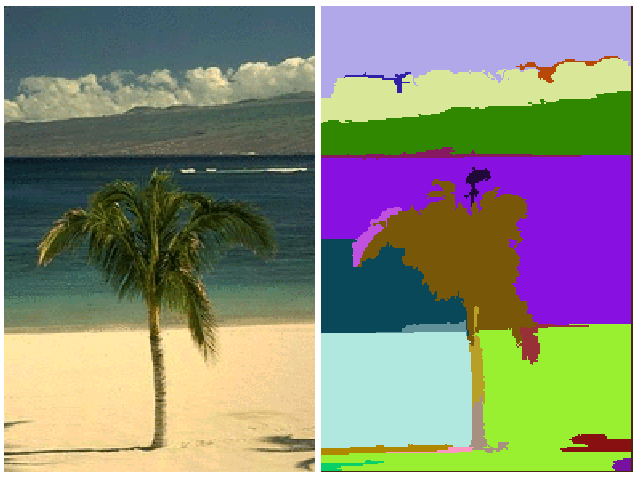
\includegraphics[width=\textwidth]{segmentation.png}
\end{figure}
\end{column}
\end{columns}
\end{frame}

\begin{frame}
Segmentation of monochrome images are based on pixel intensity properties:
\begin{itemize}
\item Discontinuities.
\item Similarity.
\end{itemize}
\end{frame}

\begin{frame}
\begin{columns}
\begin{column}{.5\textwidth}
Discontinuity:
\begin{itemize}
\item Abrupt changes in intensity levels.
\item Detection of isolated points, lines and borders.
\end{itemize}
\end{column}
\begin{column}{.5\textwidth}
Similarity:
\begin{itemize}
\item Thresholding.
\item Region growing.
\item Region division and fusion.
\end{itemize}
\end{column}
\end{columns}
\end{frame}

%\section{Detection of discontinuities}

\section{Background}

\begin{frame}
%\frametitle{Background}
\begin{itemize}
\item Three discontinuities:
\begin{enumerate}
\item Points;
\item Lines;
\item Borders.
\end{enumerate}
\item Local changes in intensity can be detected using derivatives.
\item Derivatives of a digital function are defined in terms of differences.
\end{itemize}
\end{frame}

\begin{frame}
\begin{columns}
\begin{column}{.5\textwidth}
\begin{itemize}
%\item Abrupt local changes in intensity can be detected using derivatives.
\item Approximations of first derivative must be:
\begin{enumerate}
\item Zero in regions of constant intensity;
\item Nonzero on the onset of an intensity step or ramp;
\item Nonzero at points along an intensity ramp.
\end{enumerate}
\end{itemize}
\end{column}
\begin{column}{.5\textwidth}
\begin{itemize}
\item Approximations of second derivatives must be:
\begin{enumerate}
\item Zero in regions of constant intensity;
\item Nonzero at the onset \textit{and} end of an intensity step or ramp;
\item Zero along intensity ramps.
\end{enumerate}
\end{itemize}
\end{column}
\end{columns}
\end{frame}

\begin{frame}
\begin{figure}[!h]
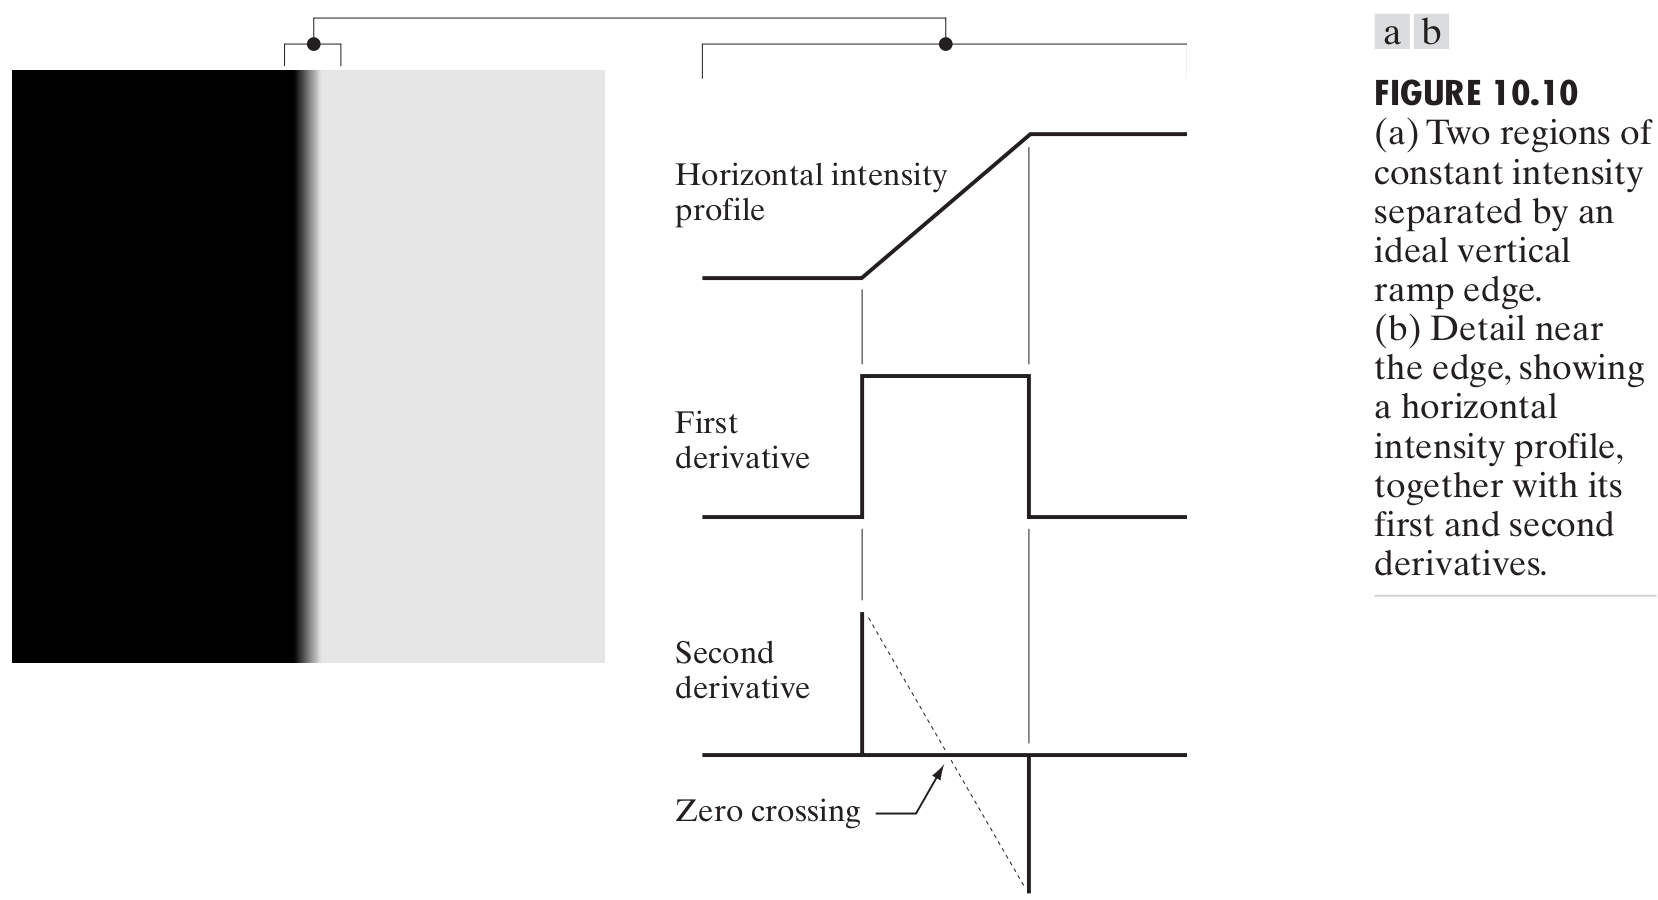
\includegraphics[width=\textwidth]{fig-10-10.png}
\end{figure}
\end{frame}

\begin{frame}
First order derivative approximation:
\begin{equation}
\dfrac{\partial f}{\partial x} = f'(x) = f(x+1) - f(x).
\end{equation}
Second order derivative approximation:
\[
\dfrac{\partial^{2}f}{\partial x^{2}} = \dfrac{\partial f'(x)}{\partial x} = f'(x+1) - f'(x)
\]
\[
= f(x+2) - f(x+1) - f(x+1) + f(x)
\]
\[
= f(x+2) -2f(x+1) + f(x)
\]
\begin{equation}
\dfrac{\partial^{2}f}{\partial x^{2}} = f''(x) = f(x+1) + f(x-1) - 2 f(x).
\end{equation}
\end{frame}

\begin{frame}
\begin{figure}[!h]
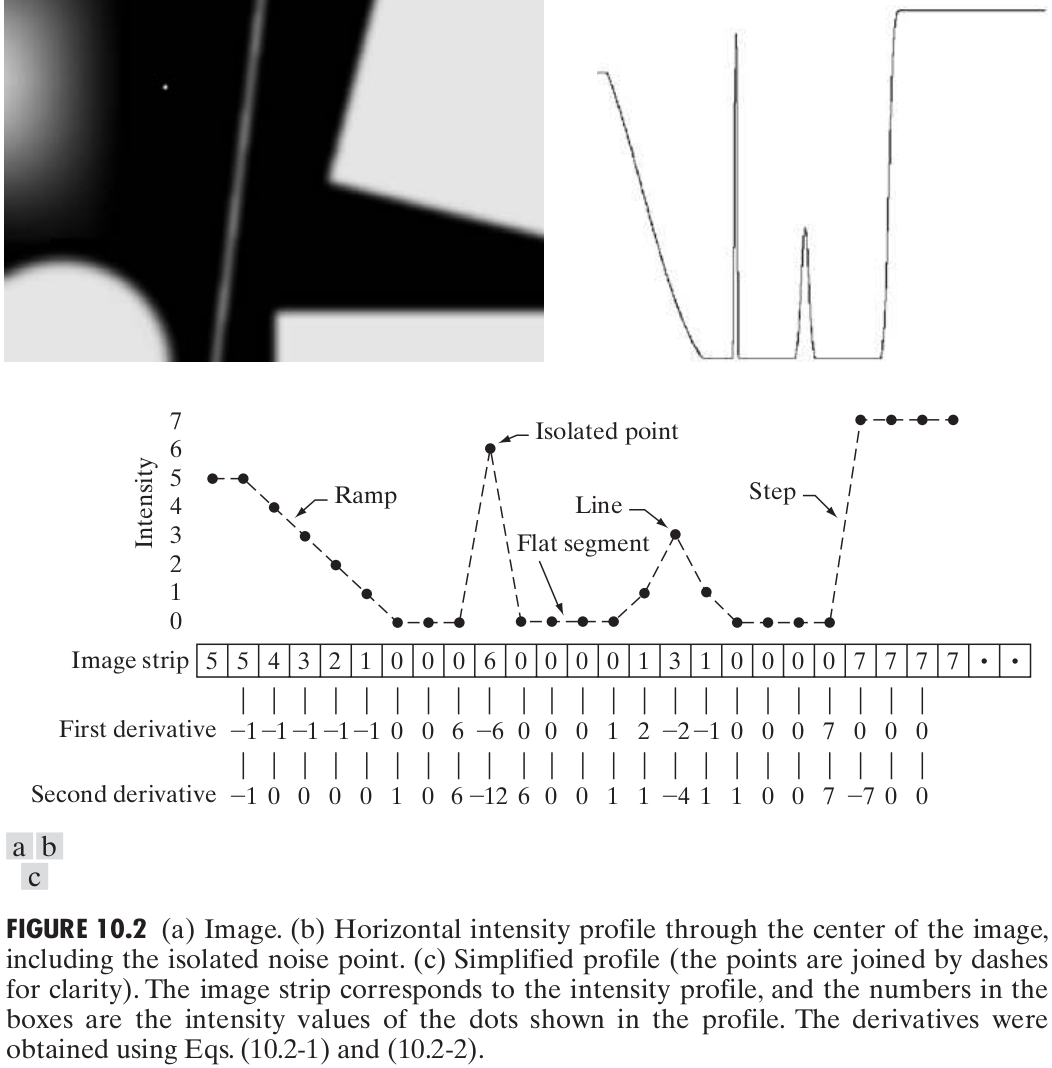
\includegraphics[width=.7\textwidth]{fig-10-2.png}
\end{figure}
\end{frame}

\begin{frame}
To find derivatives we scan the image using a mask.
\[
R = w_{1}z_{1} + w_{2}z_{2} + \ldots	+ w_{9}z_{9}
\]
\[
R = \sum_{k=1}^{9} w_{k}z_{k}
\]
$z_{i}$ is the gray-scale intensity of \textit{pixel} associated with the coefficient $w_{i}$ of the mask.
\begin{figure}[!h]
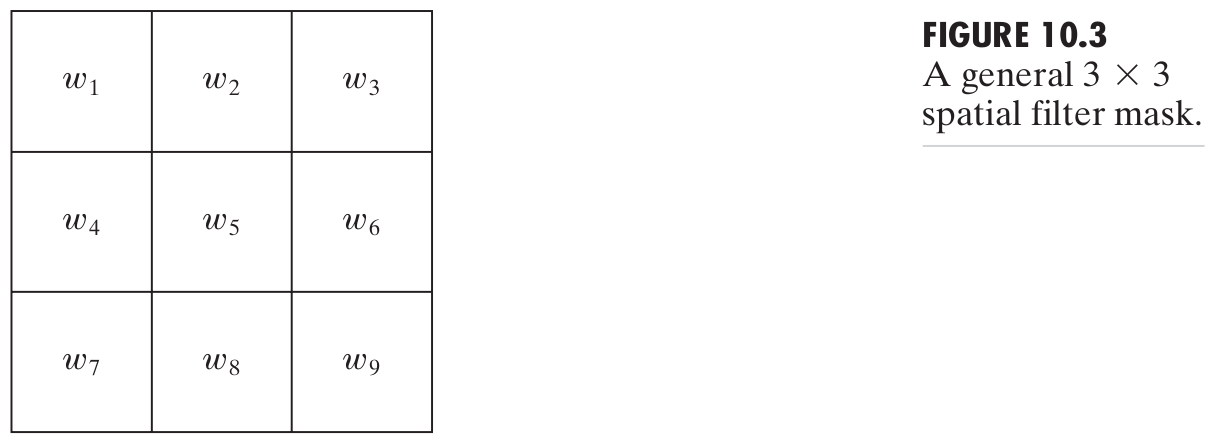
\includegraphics[width=.8\textwidth]{fig-10-3.png}
\end{figure}
\end{frame}

\section{Point, line and edge detection}

\subsection{Point detection}

\begin{frame}
%\frametitle{Point detection}
Points are detected based on the Laplacian:
\[
\nabla^{2} f(x,y) = \dfrac{\partial^{2}f(x,y)}{\partial x} + \dfrac{\partial^{2} f(x,y)}{\partial y}
\]
\begin{equation}
\nabla^{2} f(x,y) = f(x+1,y) + f(x-1,y) + f(x,y+1) + f(x,y-1) - 4f(x,y).
\end{equation}
which can be implemented by following masks:
\begin{figure}[!h]
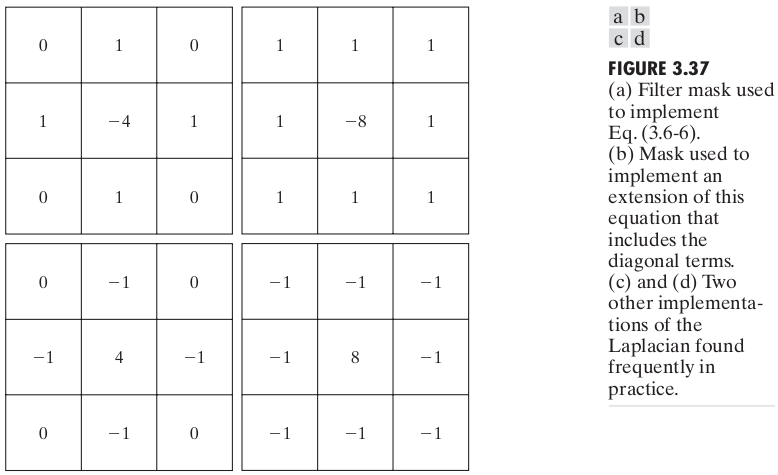
\includegraphics[width=.6\textwidth]{fig-3-37.png}
\end{figure}
\end{frame}

\begin{frame}
Example:
\begin{figure}[!h]
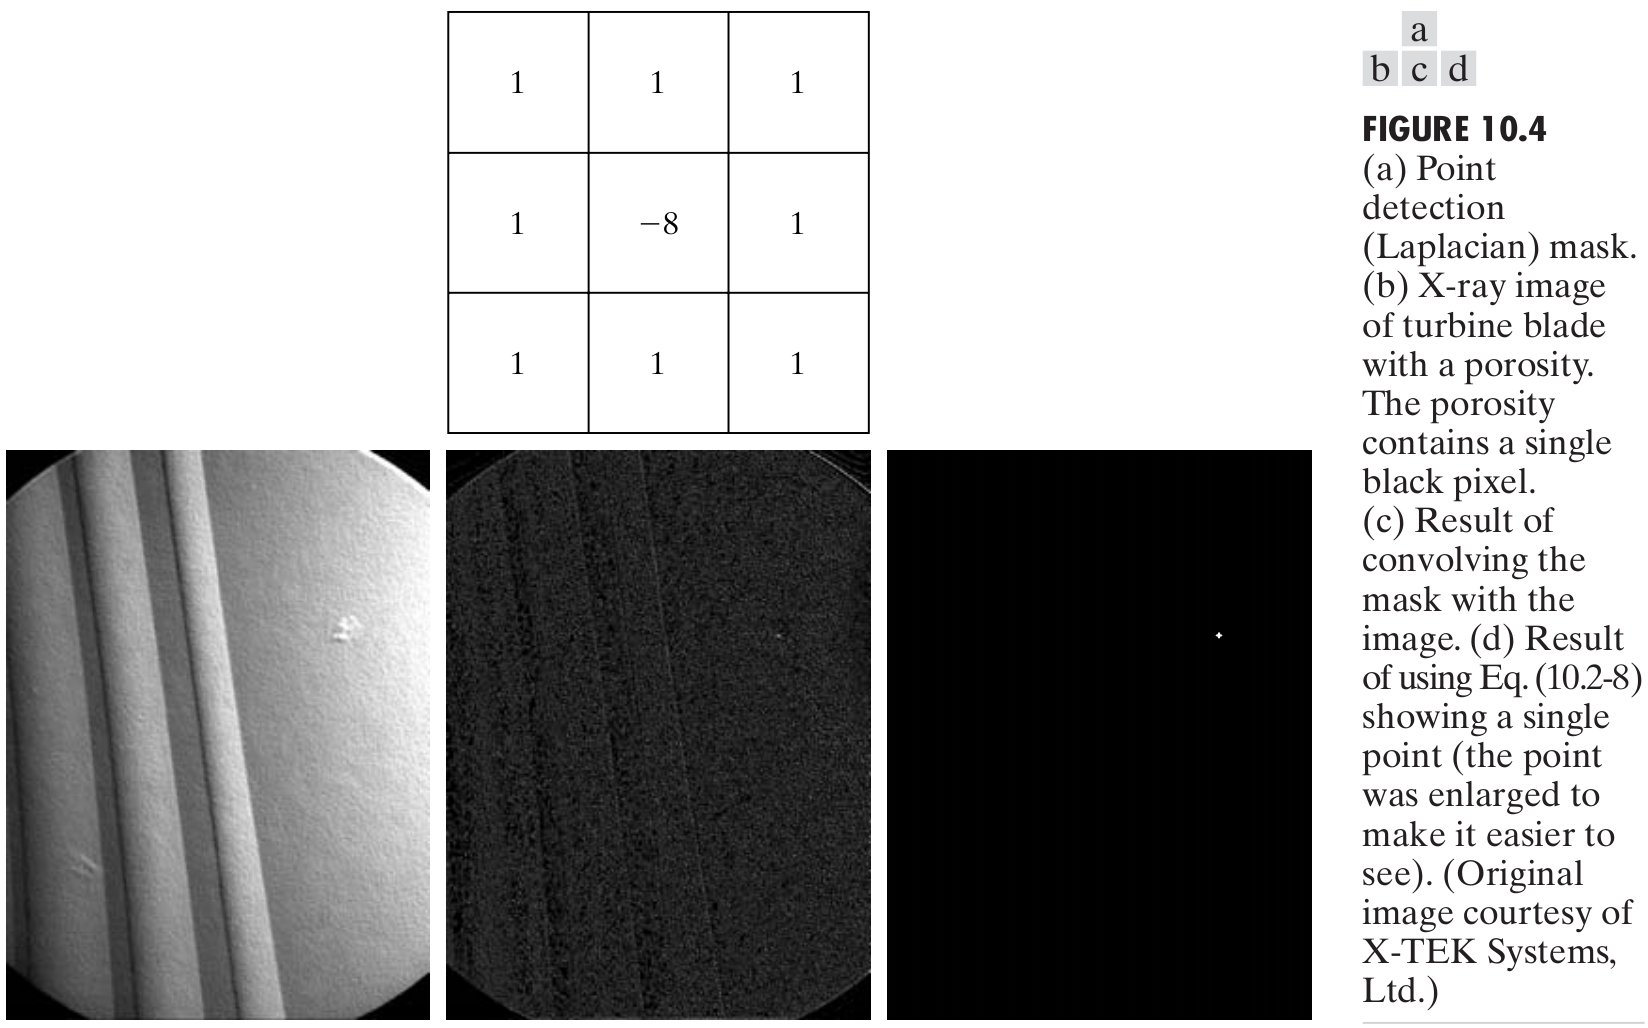
\includegraphics[width=.7\textwidth]{fig-10-4.png}
\end{figure}
\begin{itemize}
\item Point is detected if $R>T$, where $T$ is a threshold.
\item Weighed difference between central pixel and its neighbors.
\end{itemize}
\end{frame}

\subsection{Line detection}

\begin{frame}
%\frametitle{Line detection}
Laplacian for isotropic\footnote{Insensitive to line direction.} line detection.
\begin{figure}[!h]
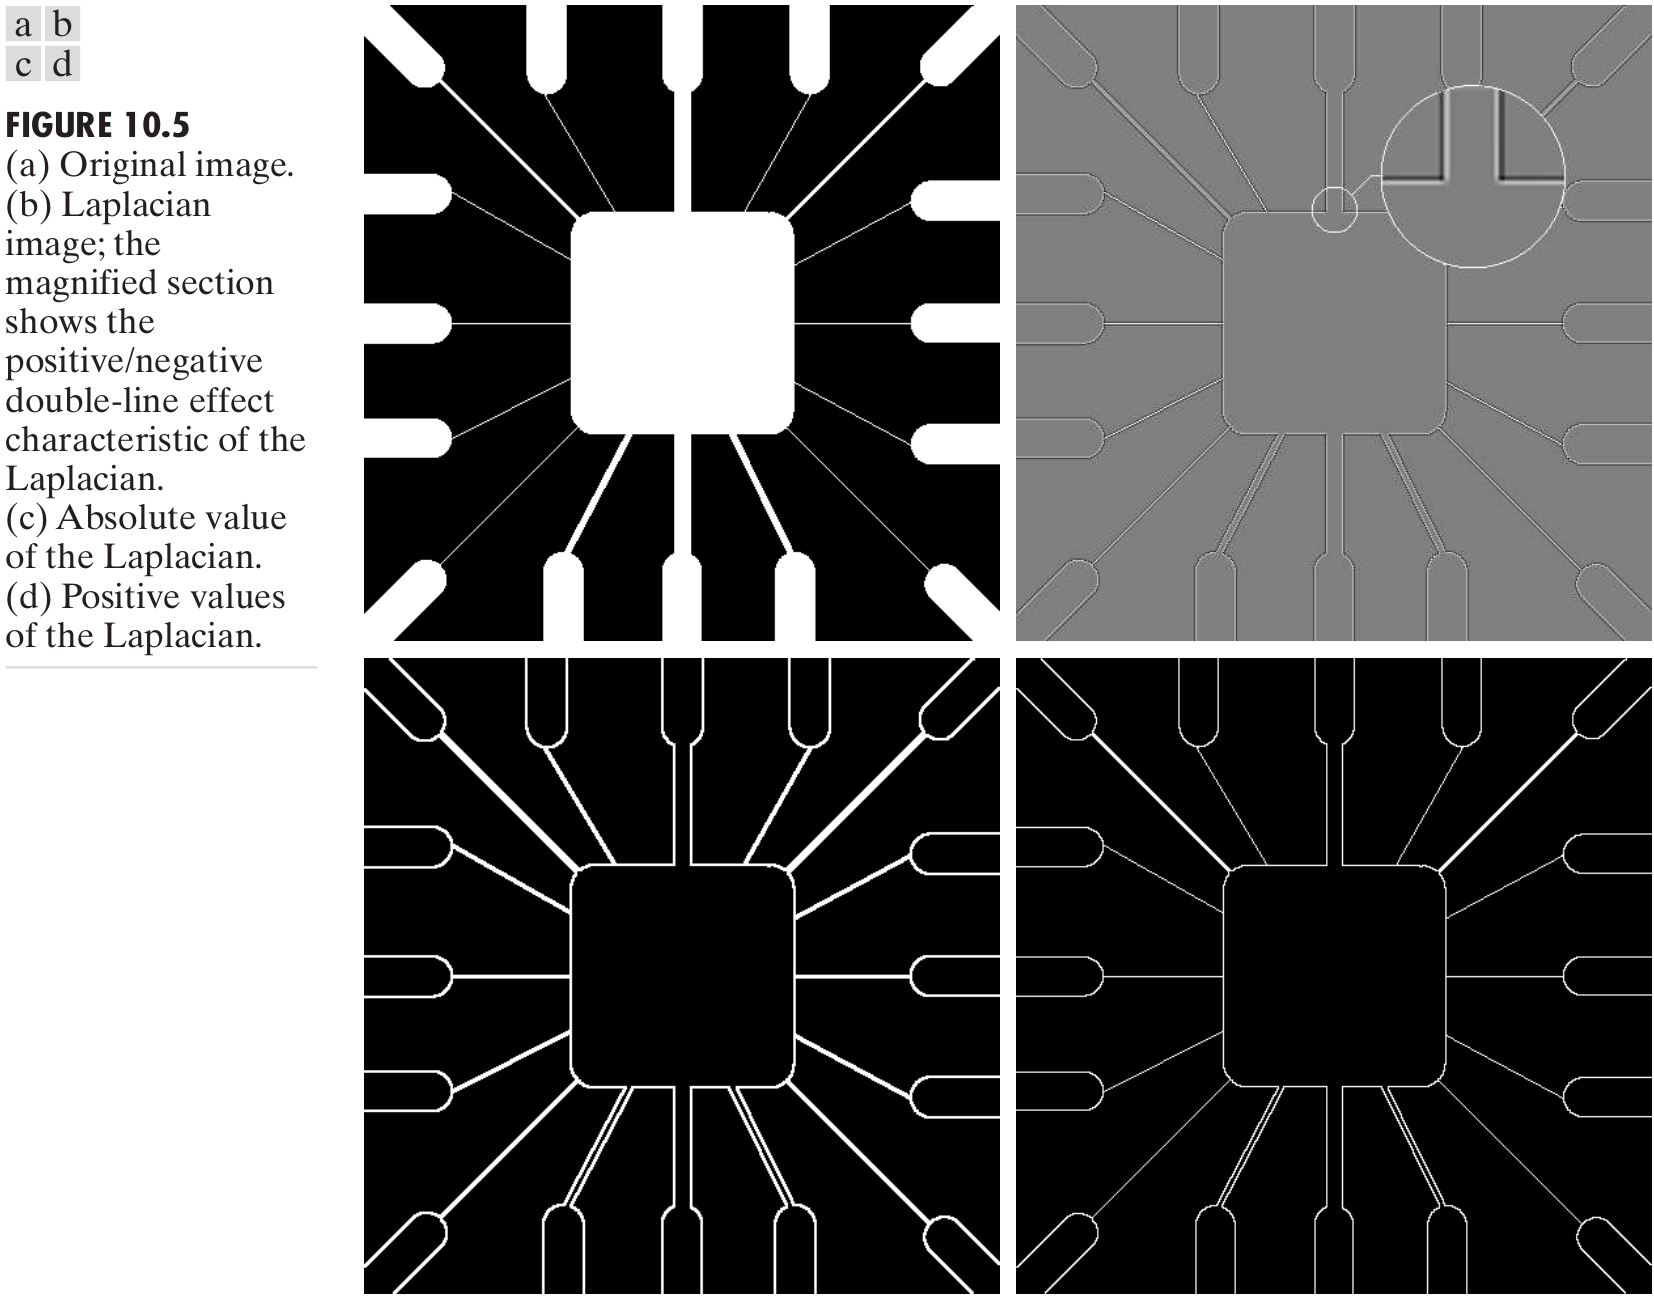
\includegraphics[width=.65\textwidth]{fig-10-5.png}
\end{figure}
\end{frame}

\begin{frame}
\begin{itemize}
\item Let $R_k,\ k=1,\ldots,4$ be the responses of the individual spatial filtering of the masks below with an image $I$.
\item For a point, if $|R_{k}| > |R_{j}|, \forall k\neq j$, then the point is more likely associated with a line with direction $k$.
\end{itemize}
\begin{figure}[!h]
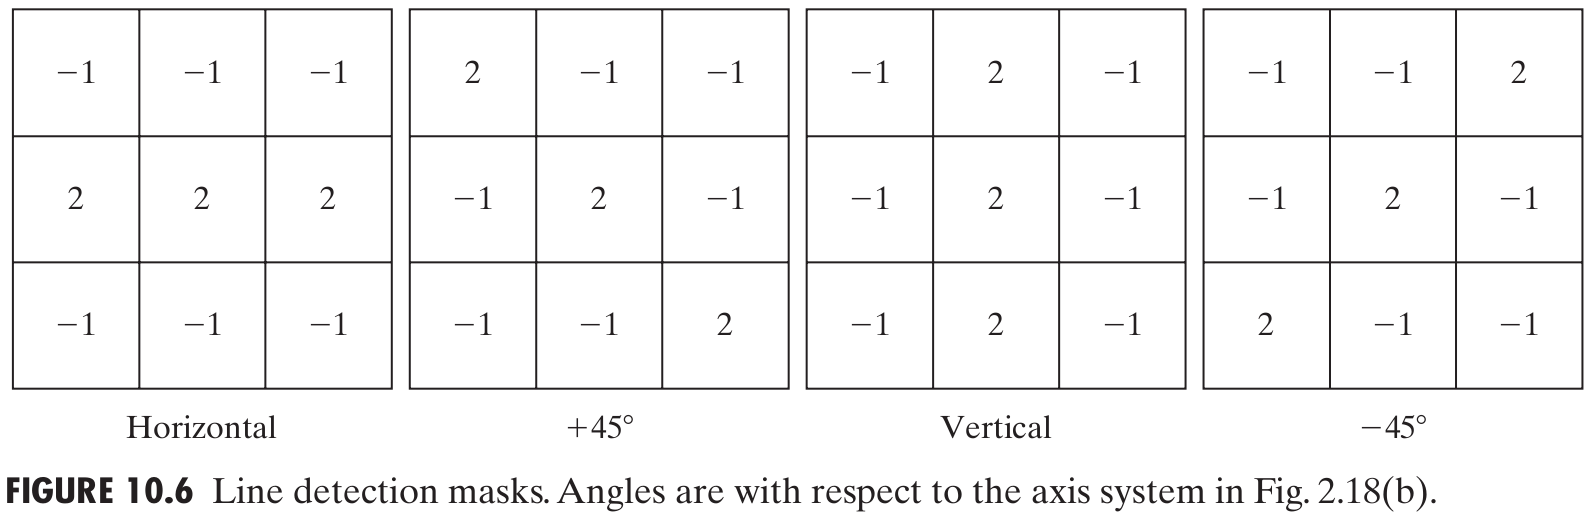
\includegraphics[width=\textwidth]{fig-10-6.png}
\end{figure}
\end{frame}

\begin{frame}
\begin{figure}[!h]
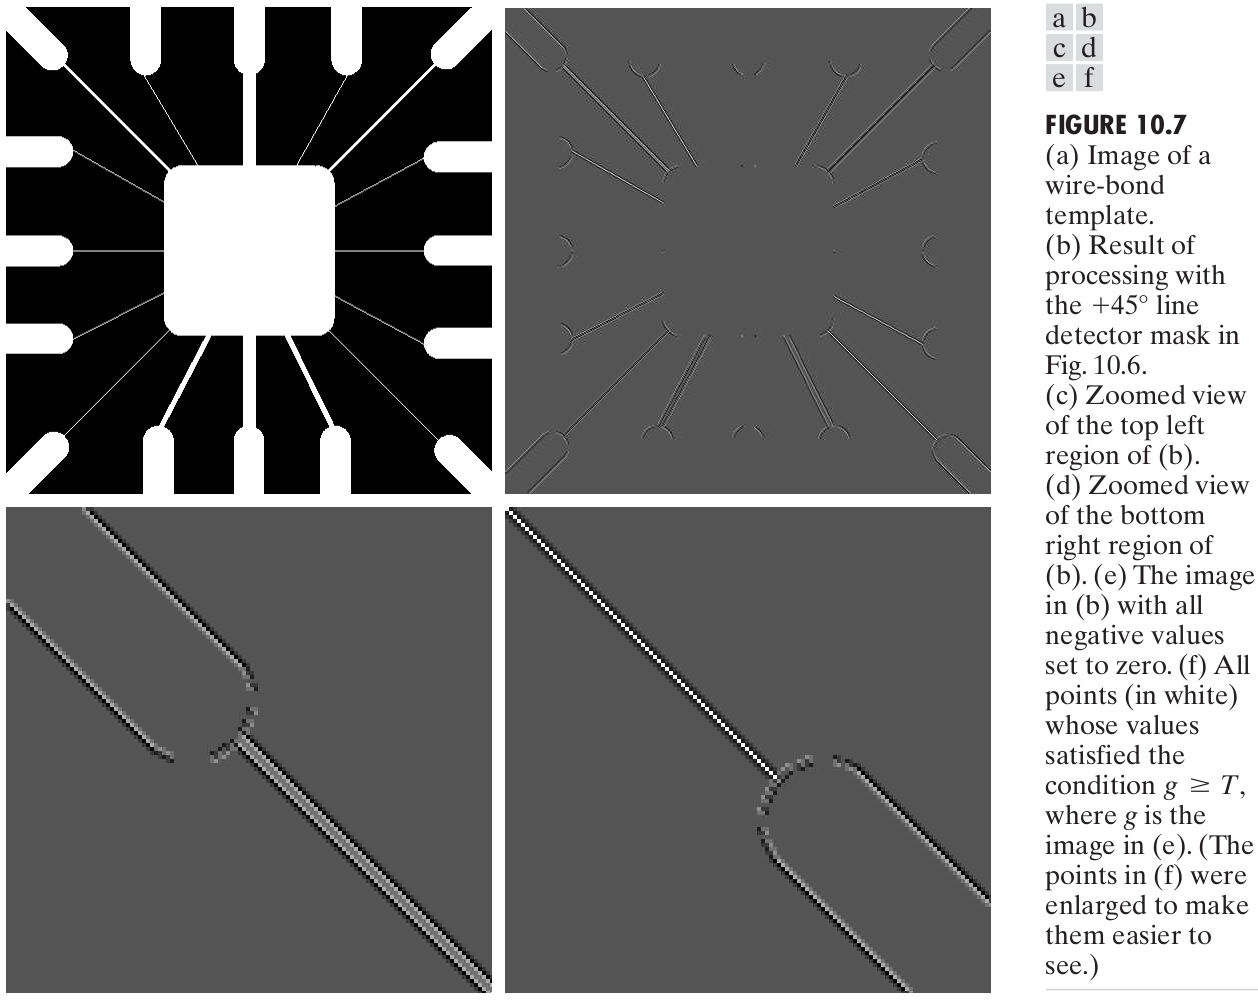
\includegraphics[width=.8\textwidth]{fig-10-7.png}
\end{figure}
\end{frame}

%\subsection{Edge models}
%
%\begin{frame}
%%\frametitle{Edge models}
%\footnotesize
%Edge models are classified according to their intensity profiles:
%\begin{itemize}
%\footnotesize
%\item Step.
%\begin{itemize}
%\footnotesize
%\item Computer generated images s.a. solid modeling and animation.
%\end{itemize}
%\item Ramp.
%\begin{itemize}
%\footnotesize
%\item Found more frequently in practice.
%\item Blurring determined by focus.
%\item Noise determined by sensor.
%\end{itemize}
%\item Roof.
%\begin{itemize}
%\footnotesize
%\item Digitization of line drawings and satellite images (roads).
%\end{itemize}
%\end{itemize}
%\normalsize
%\begin{figure}[!h]
%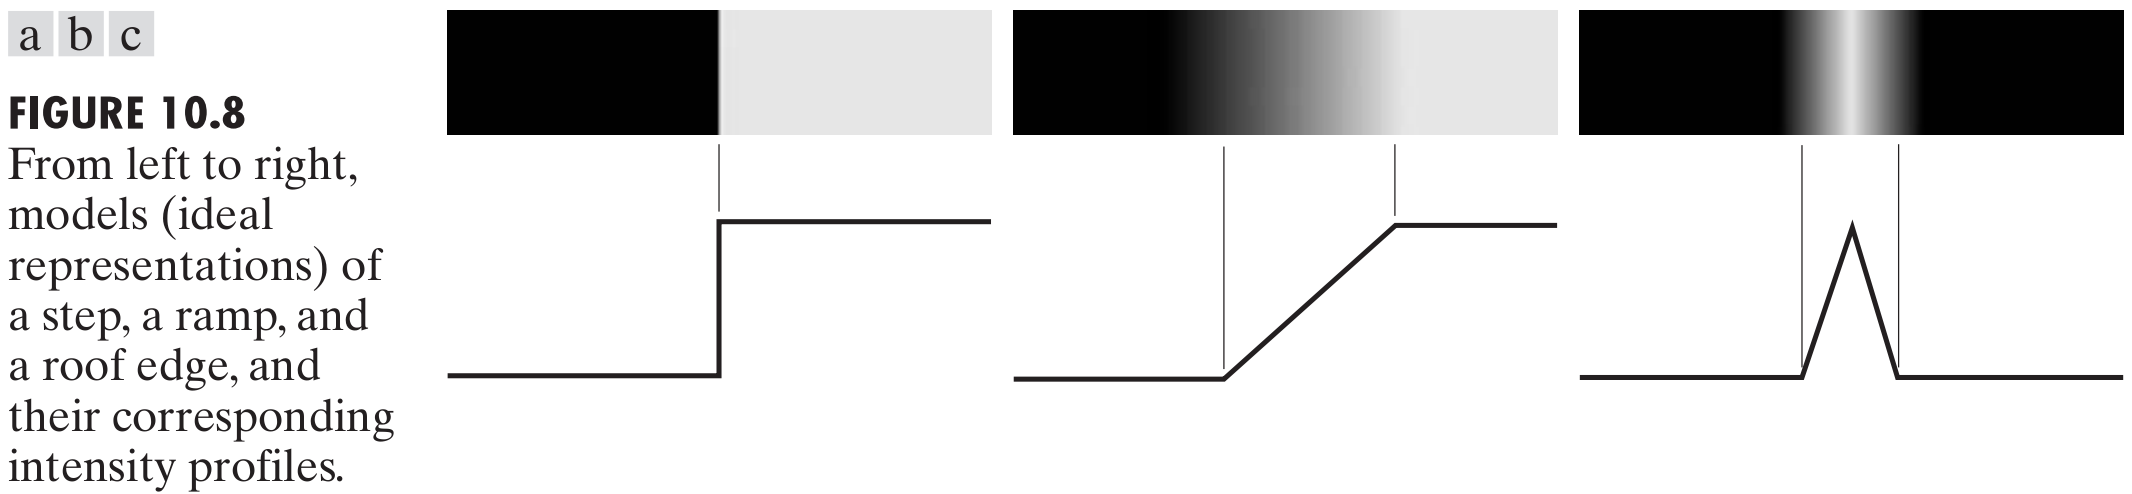
\includegraphics[width=.8\textwidth]{fig-10-8.png}
%\end{figure}
%\end{frame}
%
%\begin{frame}
%%\frametitle{Edge models}
%Not unusual to find images containing all three types of edges.
%\begin{figure}[!h]
%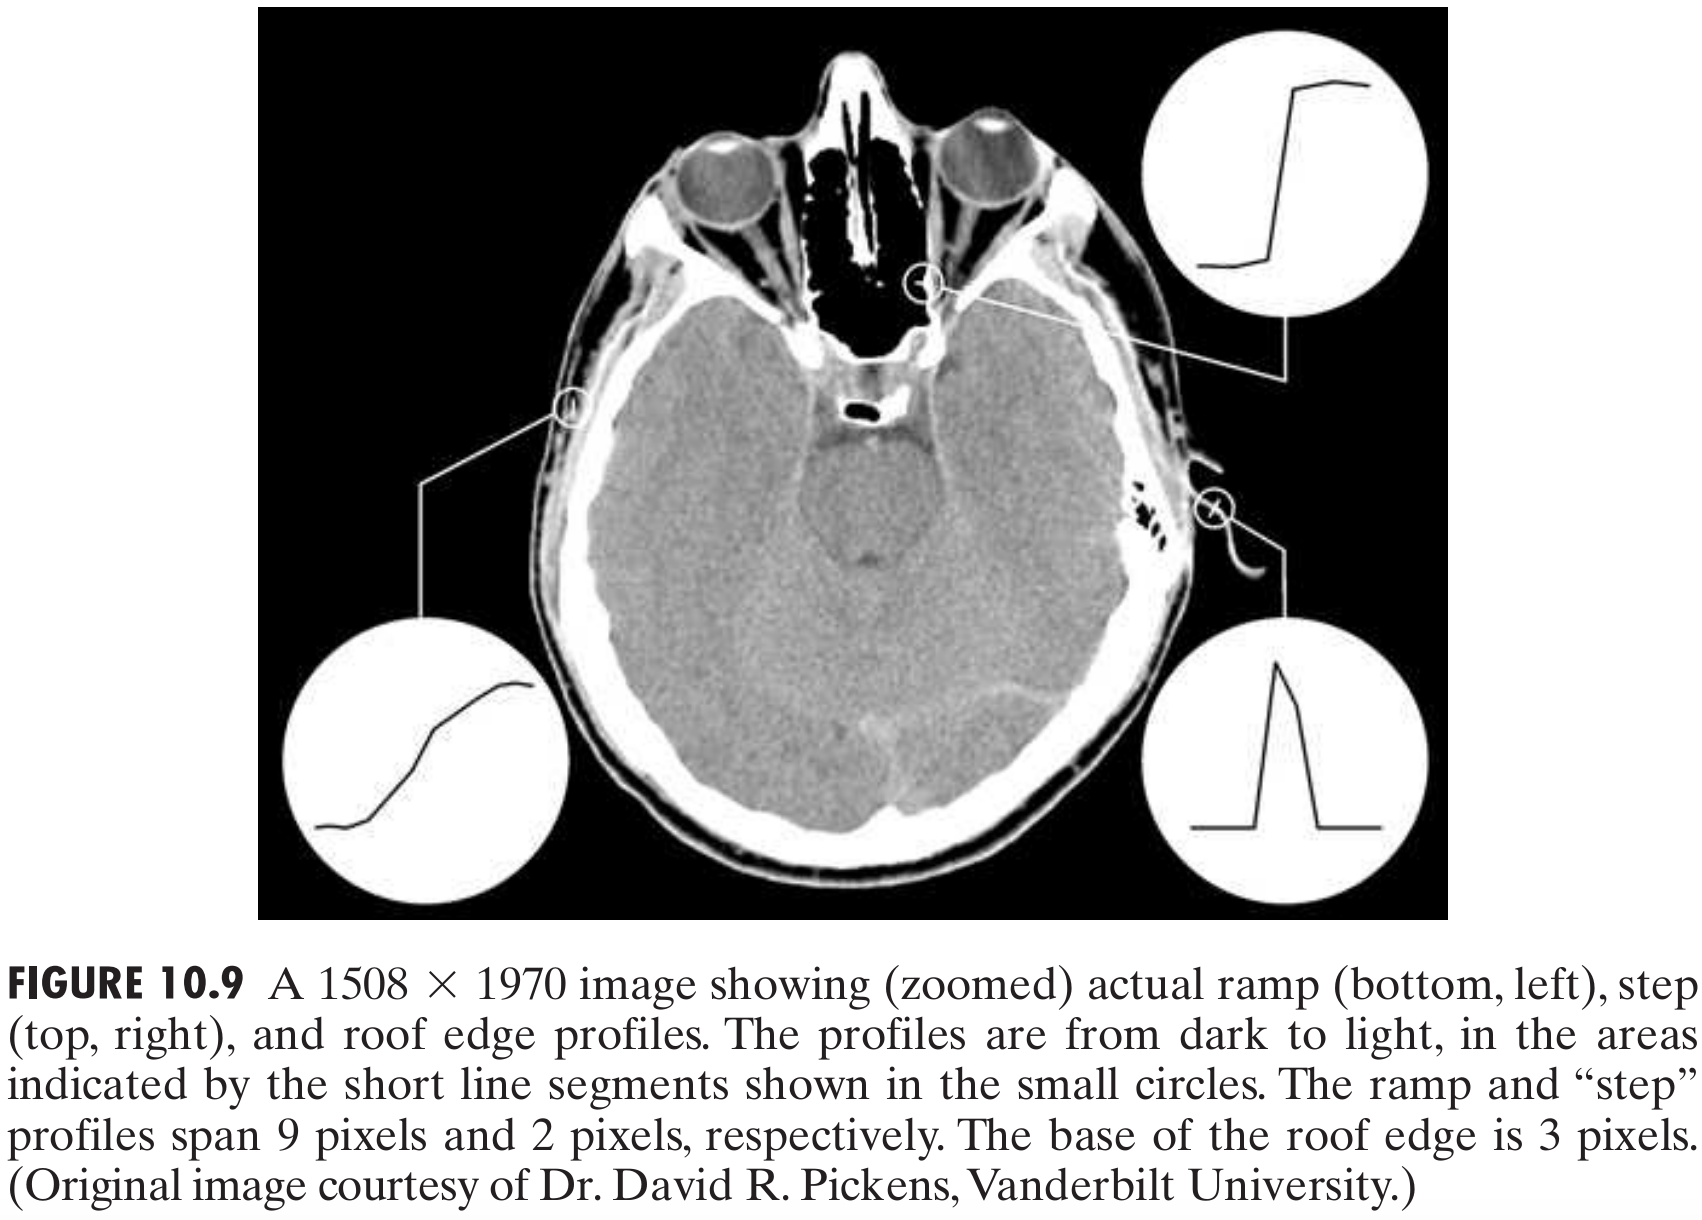
\includegraphics[width=.8\textwidth]{fig-10-9.png}
%\end{figure}
%\end{frame}
%
%\begin{frame}
%%\frametitle{Edge models}
%Properties of edge derivatives:
%\begin{itemize}
%\item The $1^{st}$ derivative indicates the presence of an edge.
%\item About the $2^{nd}$ derivative:
%\begin{enumerate}
%\item Its signs indicate bright/dark sides of the edge.
%\item It produces two values for every edge.
%\item Its zero crossing indicates the center of the edge.
%\end{enumerate}
%\end{itemize}
%\begin{figure}[!h]
%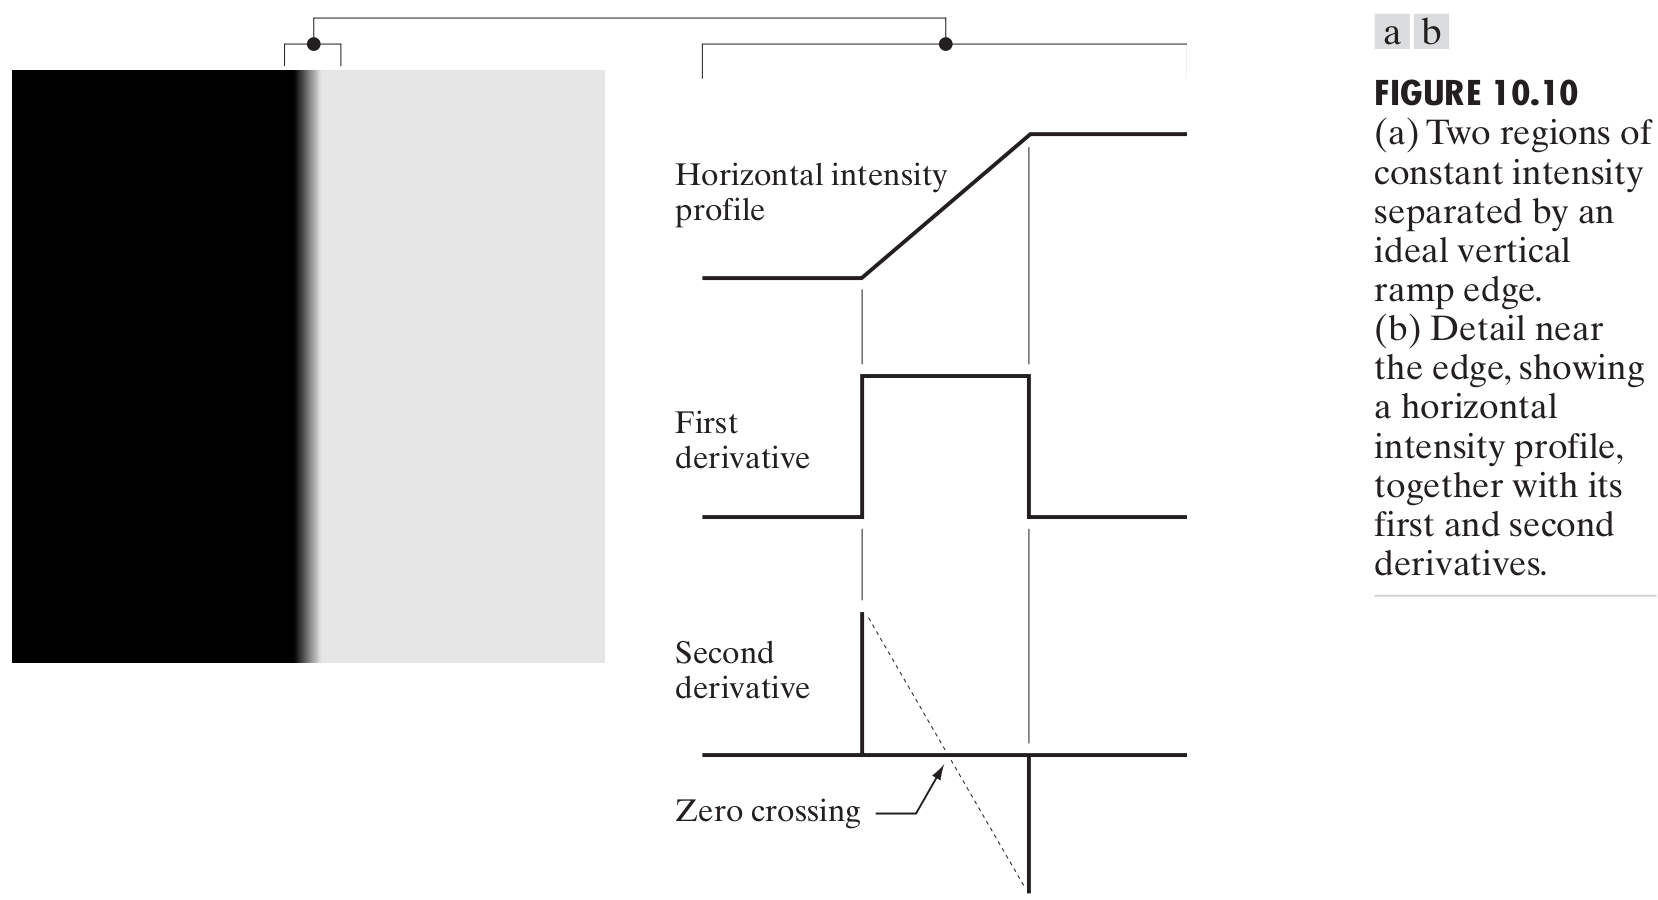
\includegraphics[width=.7\textwidth]{fig-10-10.png}
%\end{figure}
%\end{frame}
%
%\begin{frame}
%Extension to 2-D:
%\begin{figure}[!h]
%\includegraphics[width=.8\textwidth]{fig-10-11.png}
%\end{figure}
%\end{frame}
%
%\subsection{Basic edge detection}
%
%\begin{frame}
%%\frametitle{Basic edge detection}
%
%\end{frame}

\subsection{Edge models}

\begin{frame}
%\frametitle{Edge models}
\begin{itemize}
\item Step edges occur:
\begin{itemize}
\item In computer generated images (animation, solid modeling).
\end{itemize}
\item In practice, edges are blurred due to:
\begin{itemize}
\item Focus (optical apparatus).
\item Noise (electronics).
\end{itemize}
\end{itemize}
\begin{figure}[!h]
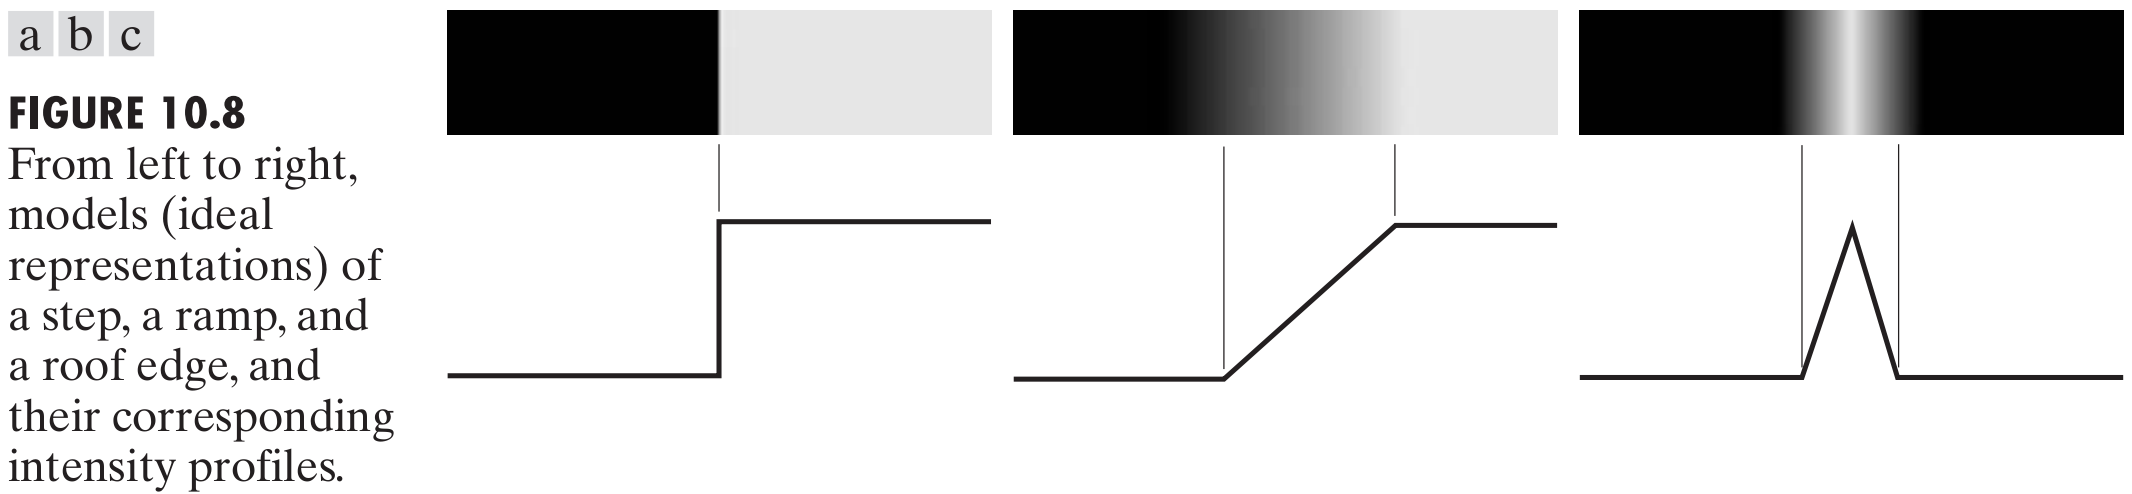
\includegraphics[width=.85\textwidth]{fig-10-8.png}
\end{figure}
\end{frame}

\begin{frame}
Images may contain all three types of edges:
\begin{figure}[!h]
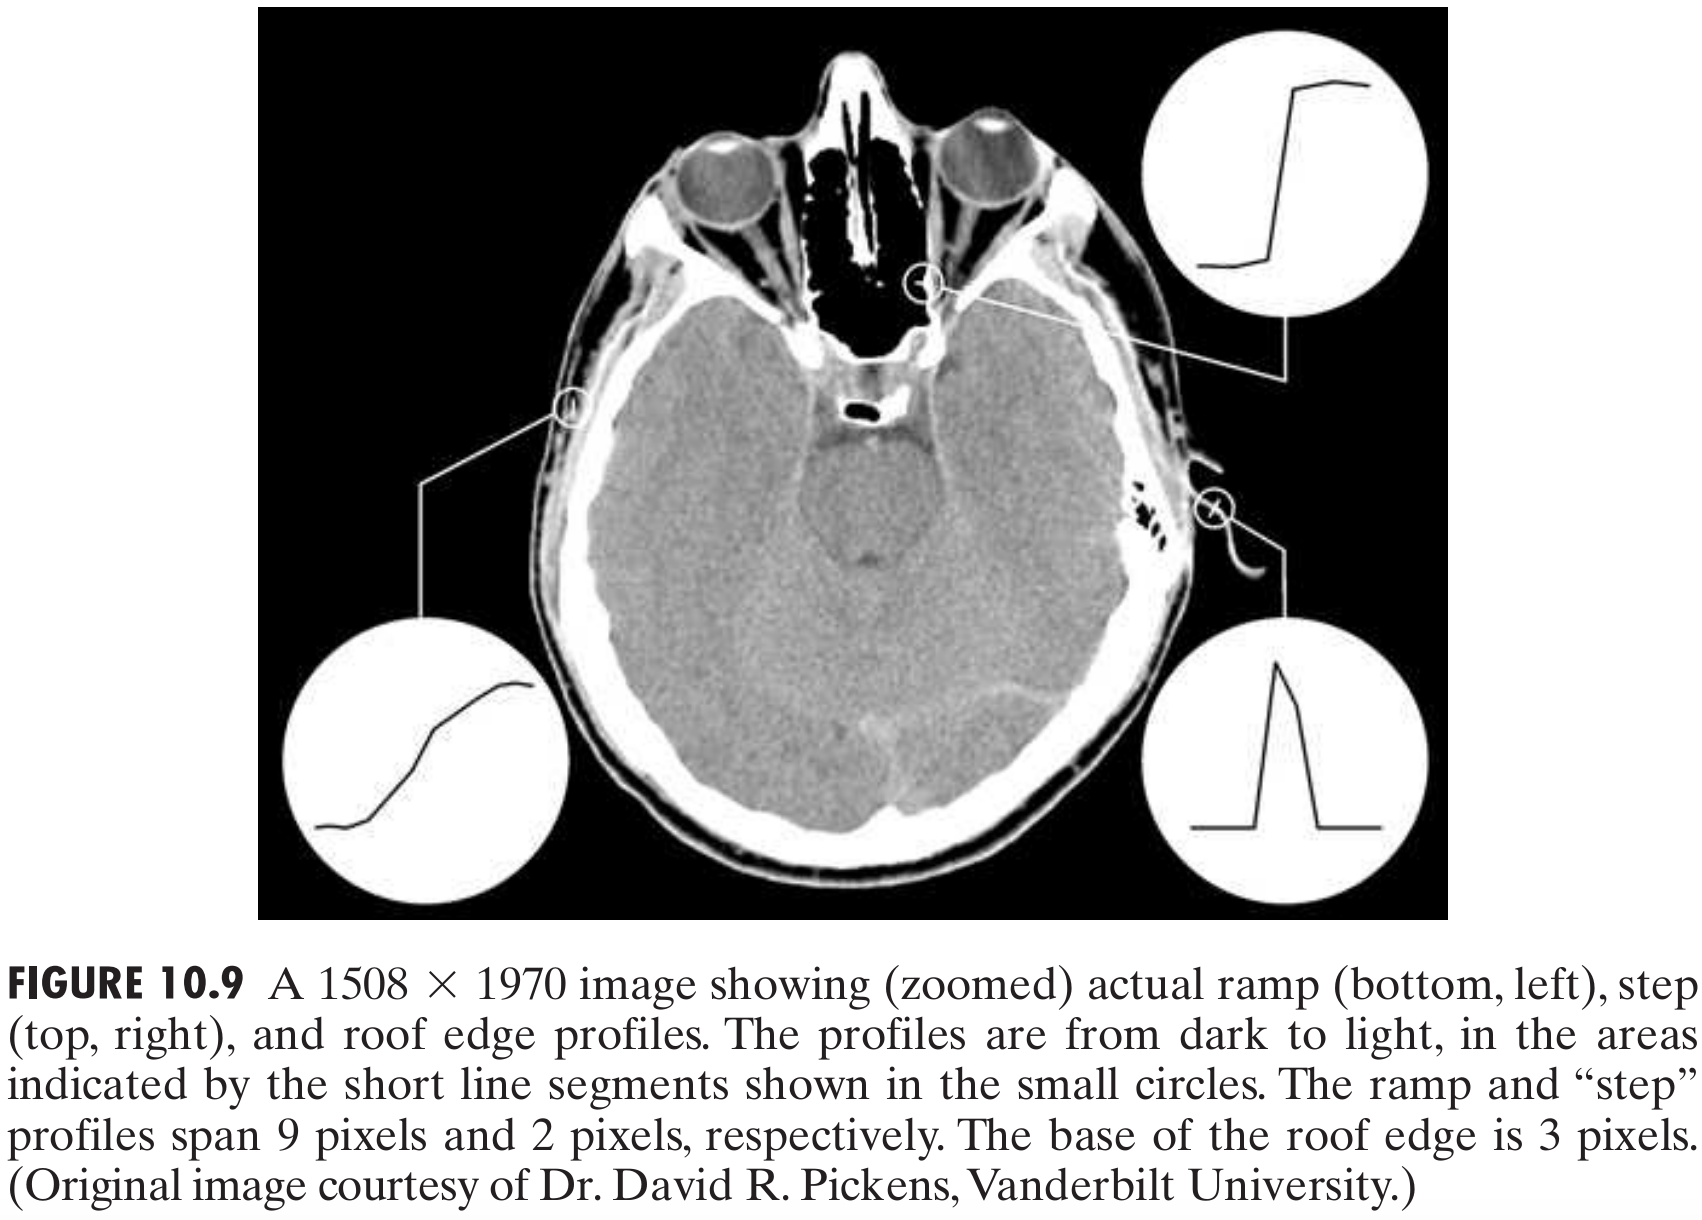
\includegraphics[width=.85\textwidth]{fig-10-9.png}
\end{figure}
\end{frame}

\begin{frame}
\begin{itemize}
\item The magnitude of the 1st der. detects an edge.
\item The 2nd derivative:
\begin{enumerate}
\item Has 2 values for an edge.
\item Its zero crossings locate the center of the edge.
\end{enumerate}
\end{itemize}
\begin{figure}[!h]
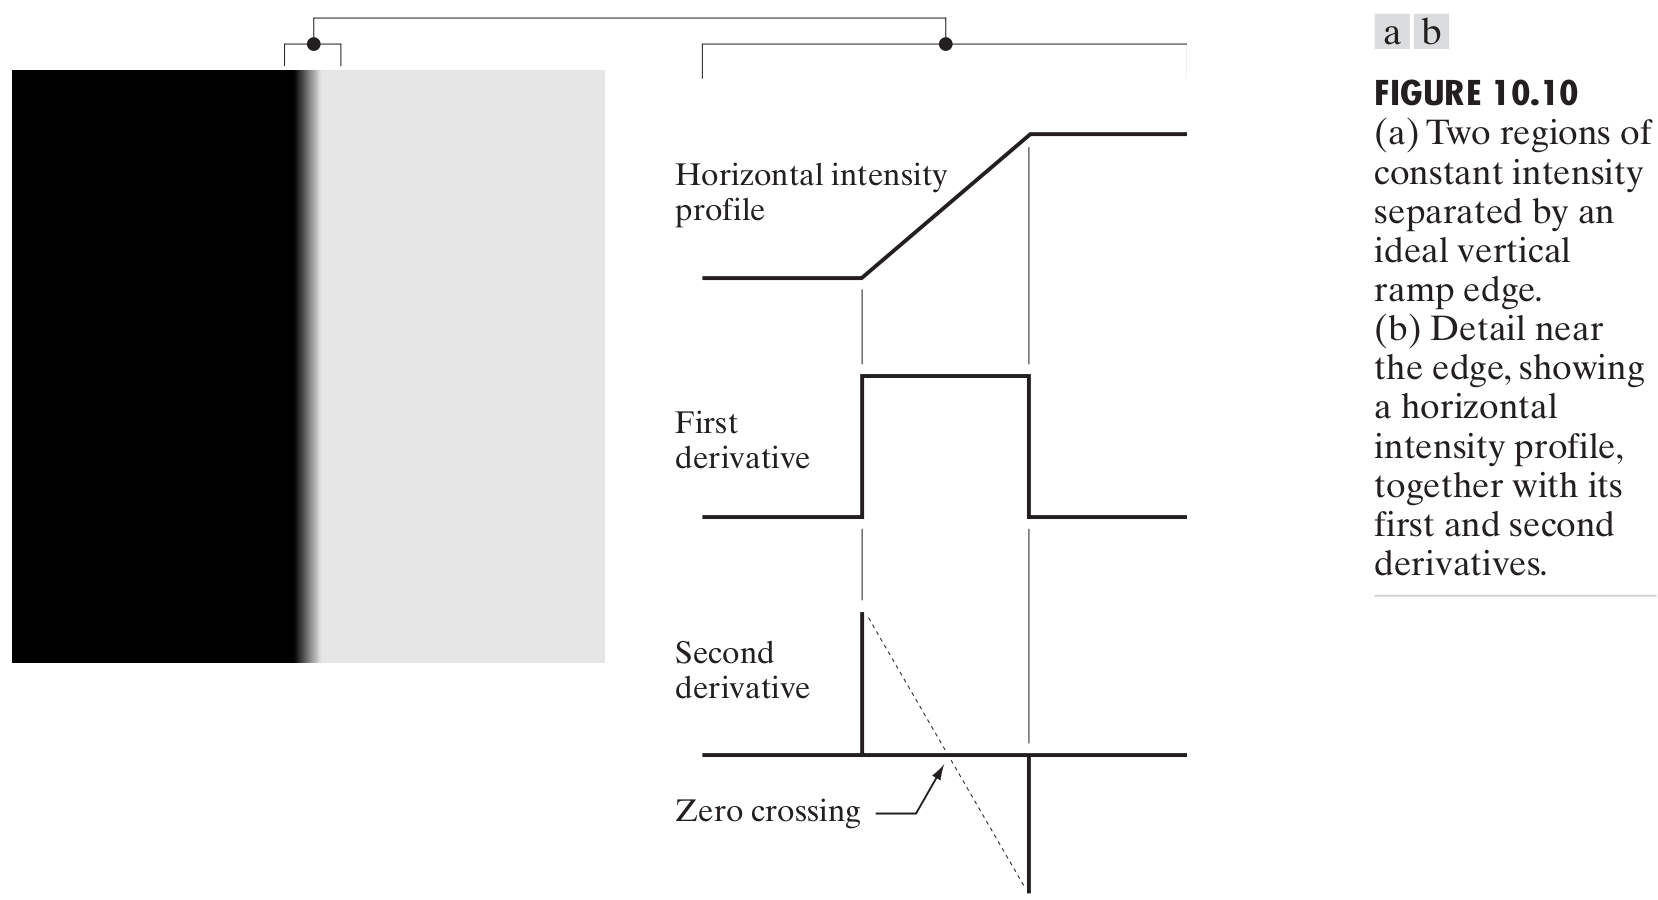
\includegraphics[width=.79\textwidth]{fig-10-10.png}
\end{figure}
\end{frame}

\begin{frame}
Problems with noisy images:
\begin{figure}[!h]
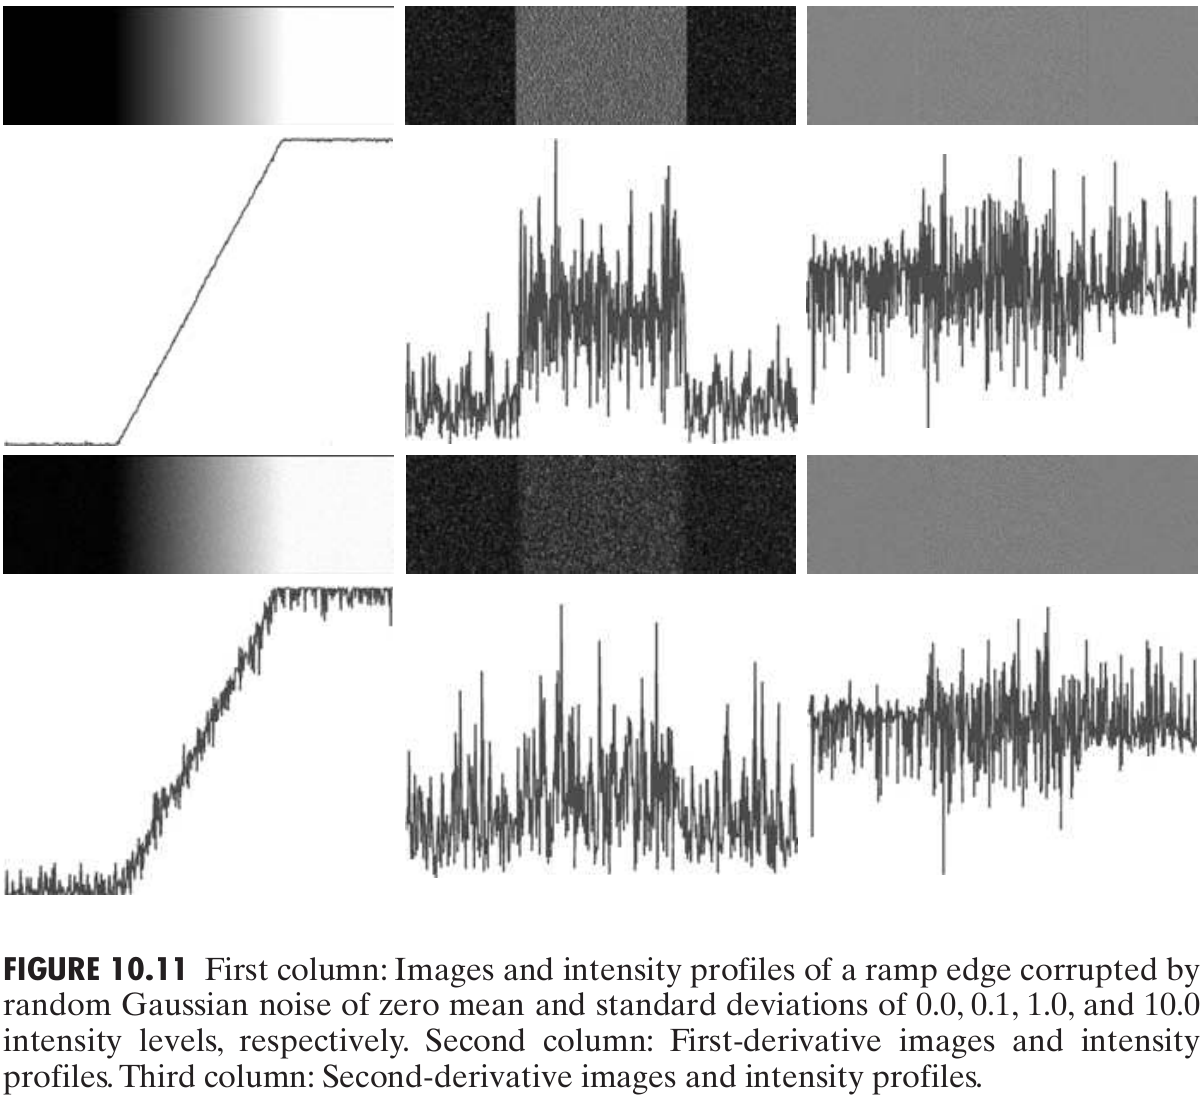
\includegraphics[width=.68\textwidth]{fig-10-11cd.png}
\end{figure}
\end{frame}

\subsection{Basic edge detection}

\begin{frame}
\frametitle{Fundamental steps in edge detection}
\begin{enumerate}
\item Image smoothing for noise reduction.
\item Detection of edge points. Local operation that detects potential edge points.
\item Edge localization. Select true members of an edge.
\end{enumerate}
\end{frame}

\subsubsection{The gradient and its properties}

\begin{frame}
%\frametitle{The gradient and its properties}
\begin{columns}
\begin{column}{.5\textwidth}
\begin{itemize}
\item First order derivative (gradient):
\[
\vec{\nabla} f \equiv % \text{grad}(f) \equiv
\left (
\begin{array}{c}
g_{x} \\
g_{y}
\end{array}
\right )
=
\left (
\begin{array}{c}
\partial f / \partial x \\
\partial f / \partial y
\end{array}
\right ).
\]
\item The \textit{magnitude}: rate of change in the direction of the gradient vector:
\[
| \vec{\nabla} f | = M(x,y) = \sqrt{g_{x}^{2} + g_{y}^{2}}.
\]
\end{itemize}
\end{column}
\begin{column}{.5\textwidth}
\begin{itemize}
\item The \textit{direction} of the gradient is:
\[
\alpha(x,y) = \tan^{-1}(g_{x} / g_{y}).
\]
\end{itemize}
Note: $g_{x}$, $g_{y}$ and $M$ are images the size of $f$.
\end{column}
\end{columns}
\end{frame}

\begin{frame}
%\frametitle{The gradient and its properties}
For the image below:
\begin{itemize}
\item $\nabla f = \left (
\begin{array}{c}
\partial	f / \partial x \\
\partial f / \partial y
\end{array}
\right )
=
\left (
\begin{array}{c}
-2 \\
2
\end{array}
\right )
$.
\item $M(x,y) = 2\sqrt{2}$.
\item $\alpha = \text{atan2} (g_{y} , g_{x}) = \text{atan2}  ( 2, -2 ) = 135^{\circ}$.
\end{itemize}
\begin{figure}[!h]
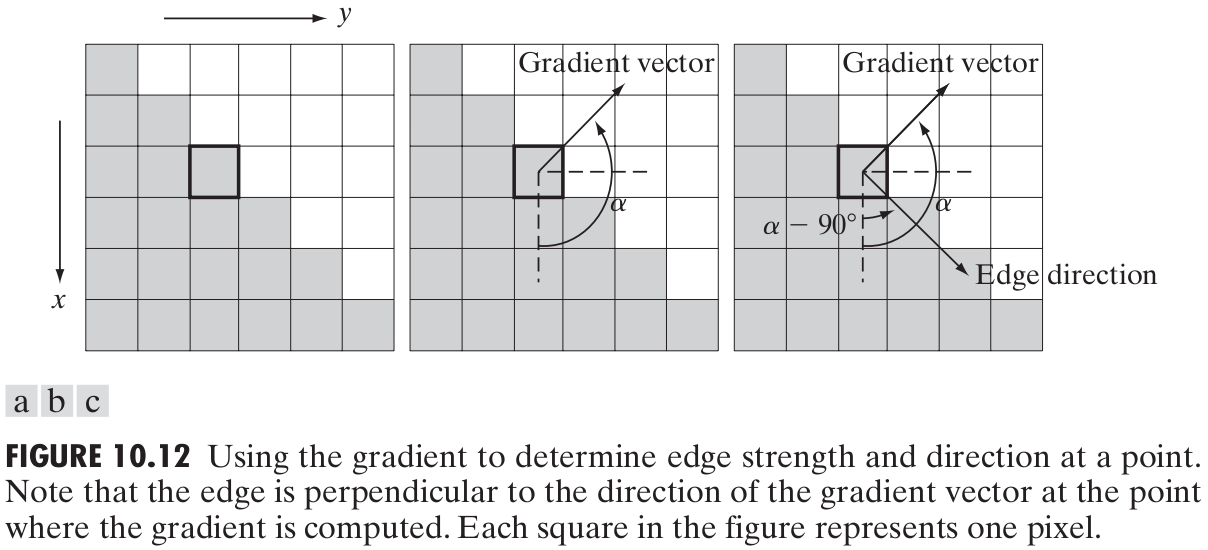
\includegraphics[width=.7\textwidth]{fig-10-12.png}
\end{figure}
\end{frame}

\subsubsection{Gradient operators}

\begin{frame}
%\frametitle{Gradient operators}
Digital approximation of first order partial derivatives:
\begin{itemize}
\item $g_{x} = \dfrac{\partial f(x,y)}{\partial x} = f(x+1, y) - f(x, y)$.
\item $g_{y} = \dfrac{\partial f(x,y)}{\partial y} = f(x, y + 1) - f(x, y)$.
\end{itemize}
\end{frame}

\begin{frame}
%\frametitle{Gradient operators}
\begin{figure}[!h]
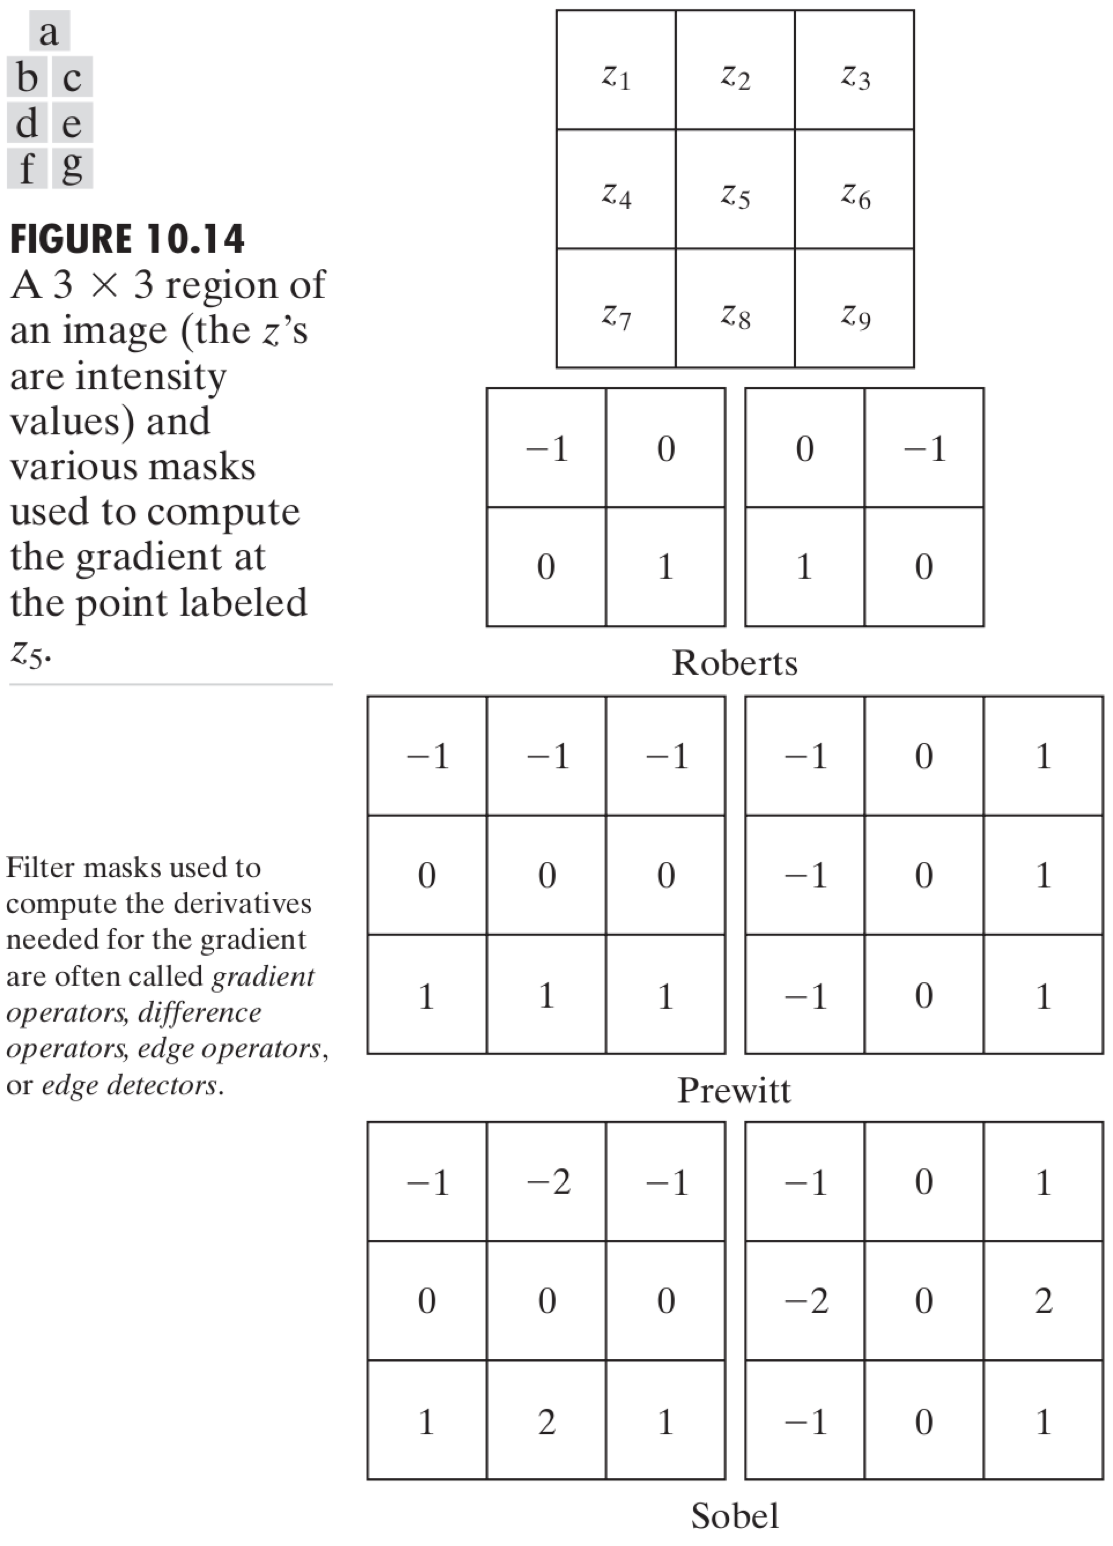
\includegraphics[width=.45\textwidth]{fig-10-14-2.png}
\end{figure}
\end{frame}

\begin{frame}
%\frametitle{Gradient operators}
Prewitt and Sobel masks for detecting diagonal edges:
\begin{figure}[!h]
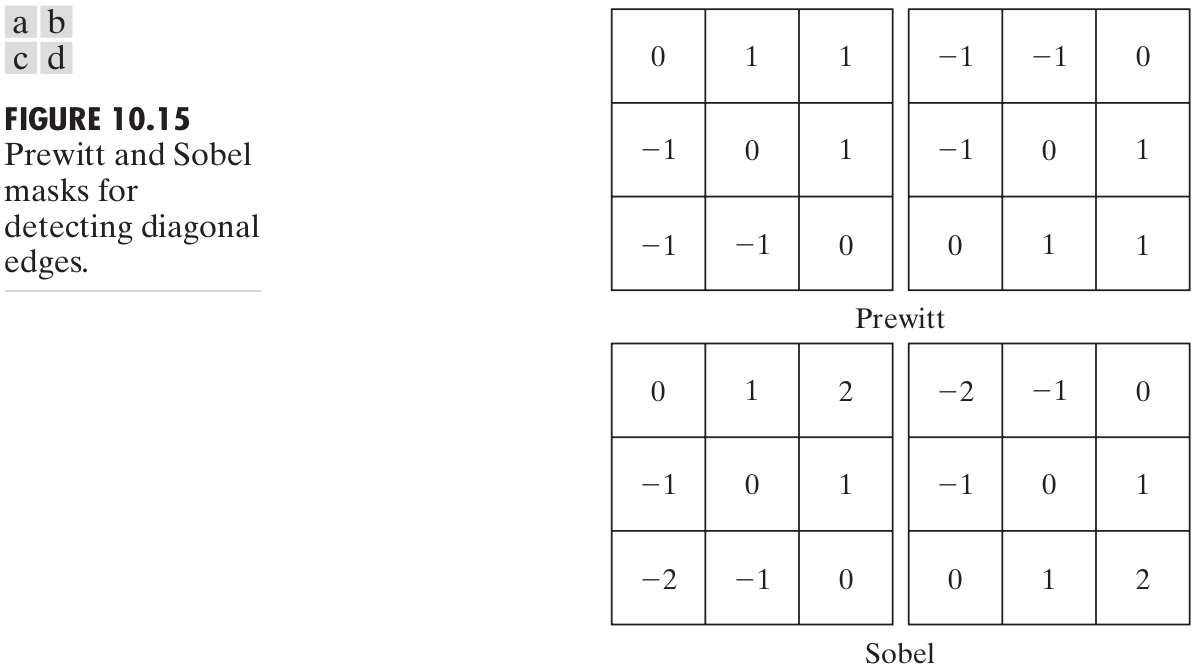
\includegraphics[width=\textwidth]{fig-10-15.png}
\end{figure}
\end{frame}

\begin{frame}
%\frametitle{Gradient operators}
\begin{columns}
\begin{column}{.5\textwidth}
\begin{itemize}
\item The presented masks are used to compute $g_{x}$ and $g_{y}$, which give edge strength \[|\nabla f| = \sqrt{g_{x}^{2} + g_{y}^{2}}\] and direction \[\alpha = \tan^{-1}(g_{y}/g_{x}).\]
\end{itemize}
\end{column}
\begin{column}{.5\textwidth}
\begin{itemize}
\item The magnitude can be approximated by
\[
M(x,y) \approx |g_{x}| + |g_{y}|;
\]
cheaper to compute but not isotropic\footnote{Invariant to rotation.}.
\end{itemize}
\end{column}
\end{columns}
\end{frame}

\begin{frame}
%\frametitle{Gradient operators}
\begin{figure}[!h]
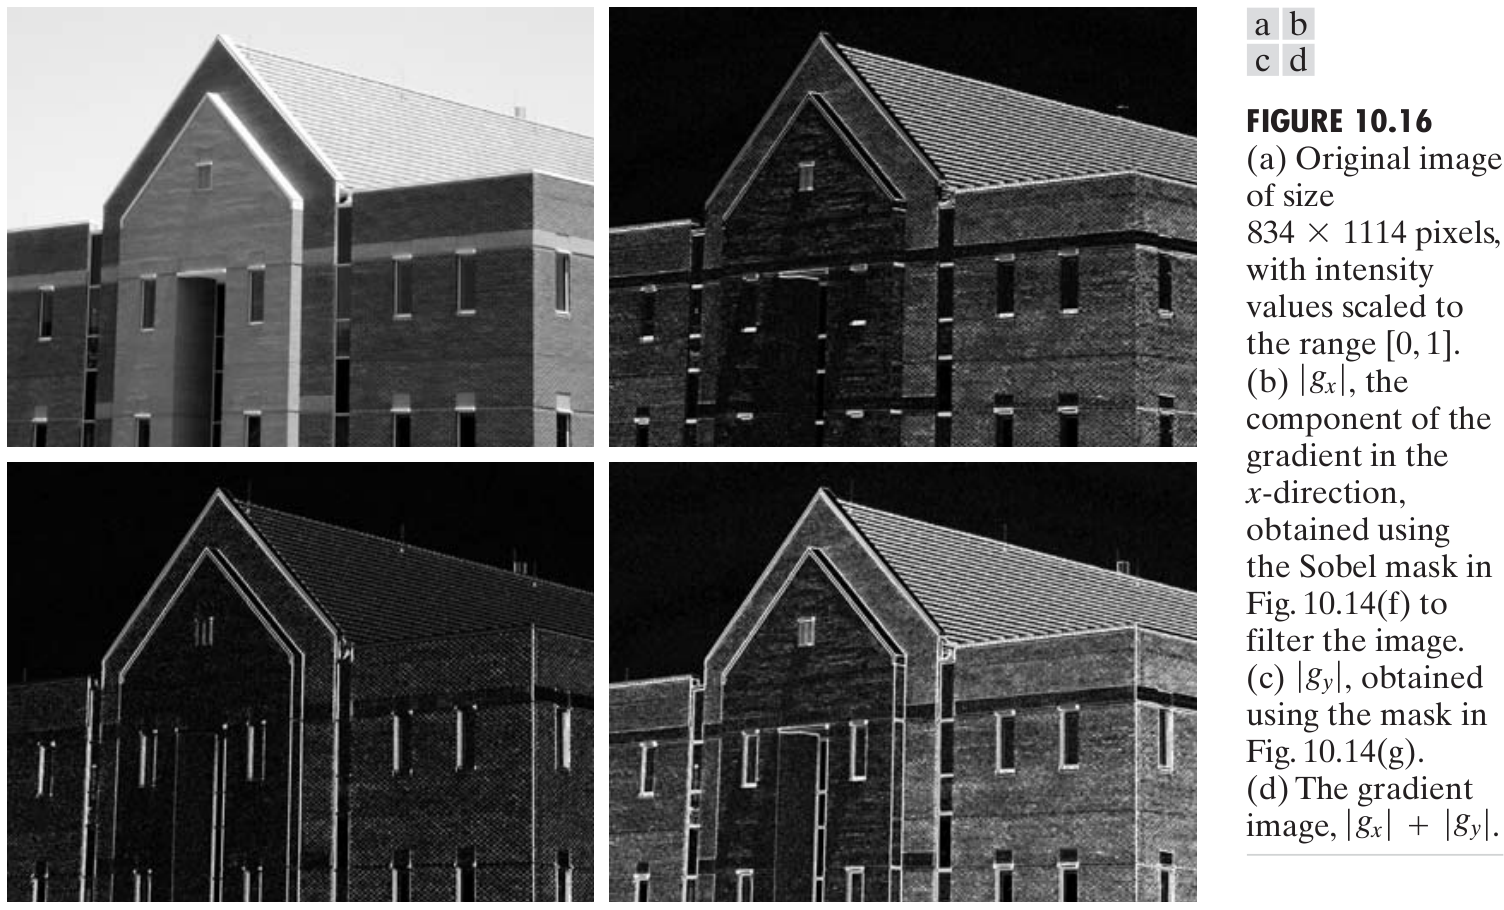
\includegraphics[width=\textwidth]{fig-10-16.png}
\end{figure}
\end{frame}

\begin{frame}
%\frametitle{Gradient operators}
The angle image ($\alpha = \tan^{-1}(g_{y}/g_{x})$):
\begin{figure}[!h]
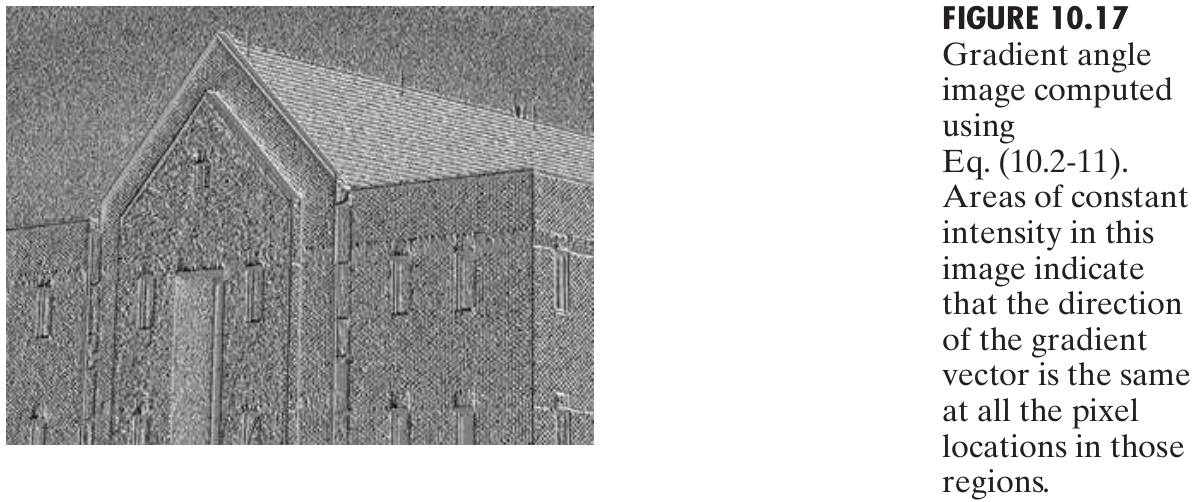
\includegraphics[width=\textwidth]{fig-10-17.png}
\end{figure}
\end{frame}

\begin{frame}
%\frametitle{Gradient operators}
Smoothing the original image to reduce detection of weak edges:
\begin{figure}[!h]
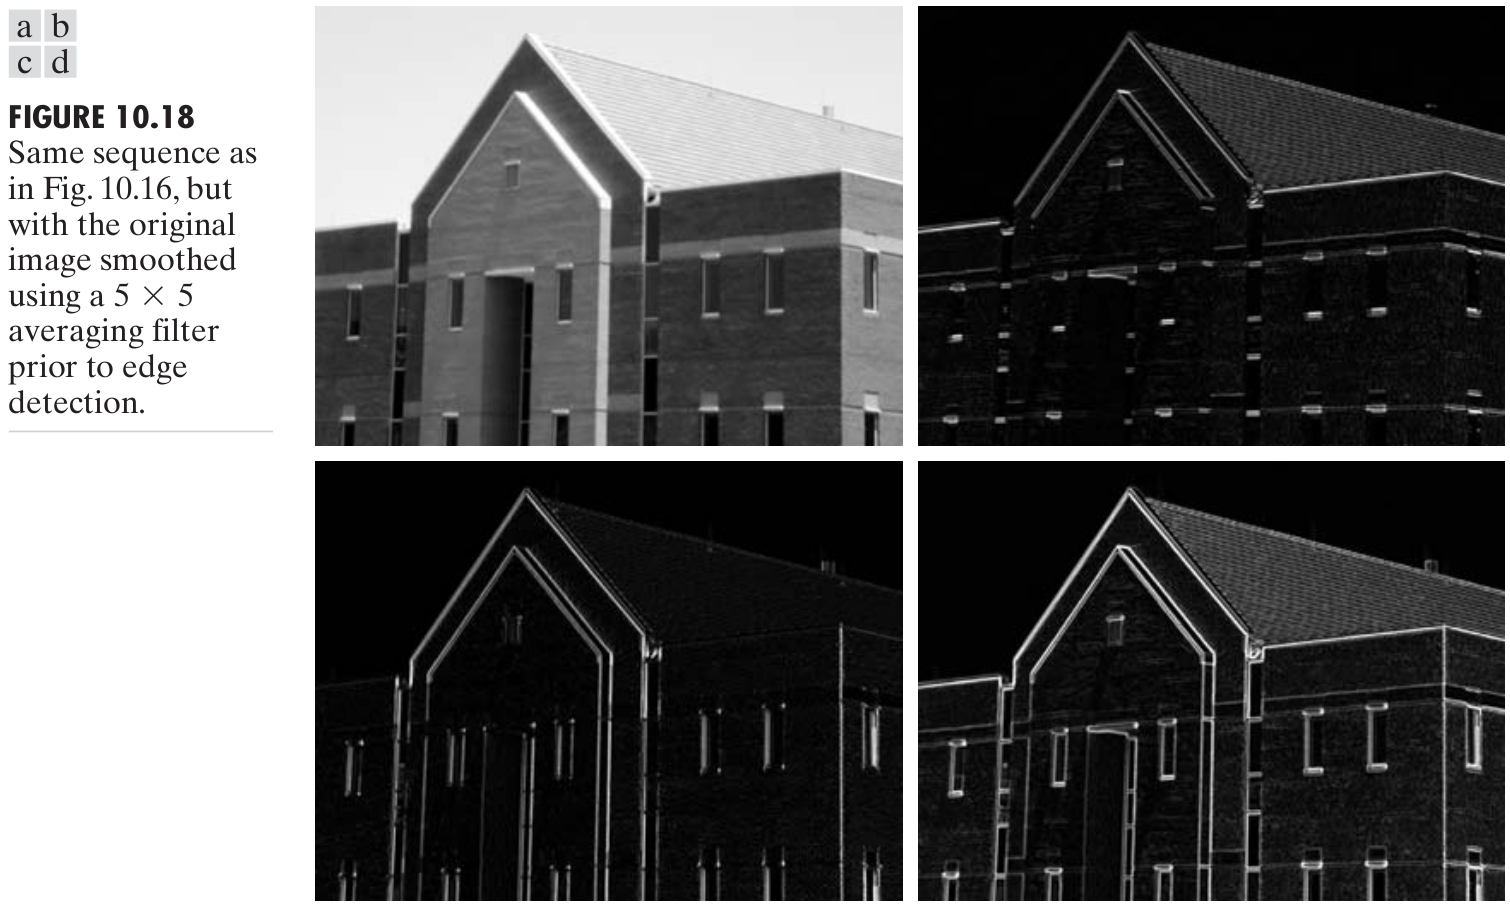
\includegraphics[width=.8\textwidth]{fig-10-18.png}
\end{figure}
\end{frame}

\begin{frame}
%\frametitle{Gradient operators}
Using diagonal masks:
\begin{figure}[!h]
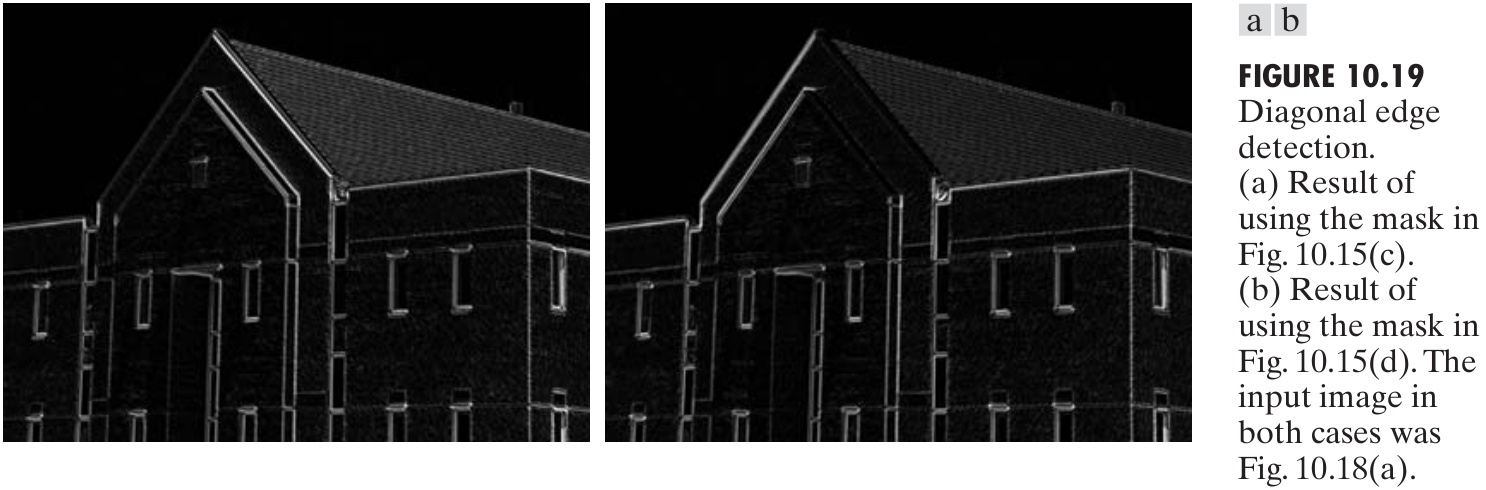
\includegraphics[width=.89\textwidth]{fig-10-19.png}
\end{figure}
\end{frame}

\subsubsection{Combining the gradient with thresholding}

\begin{frame}
%\frametitle{Combining the gradient with thresholding}
Thresholding the original and smoothed filtered images:
\begin{figure}[!h]
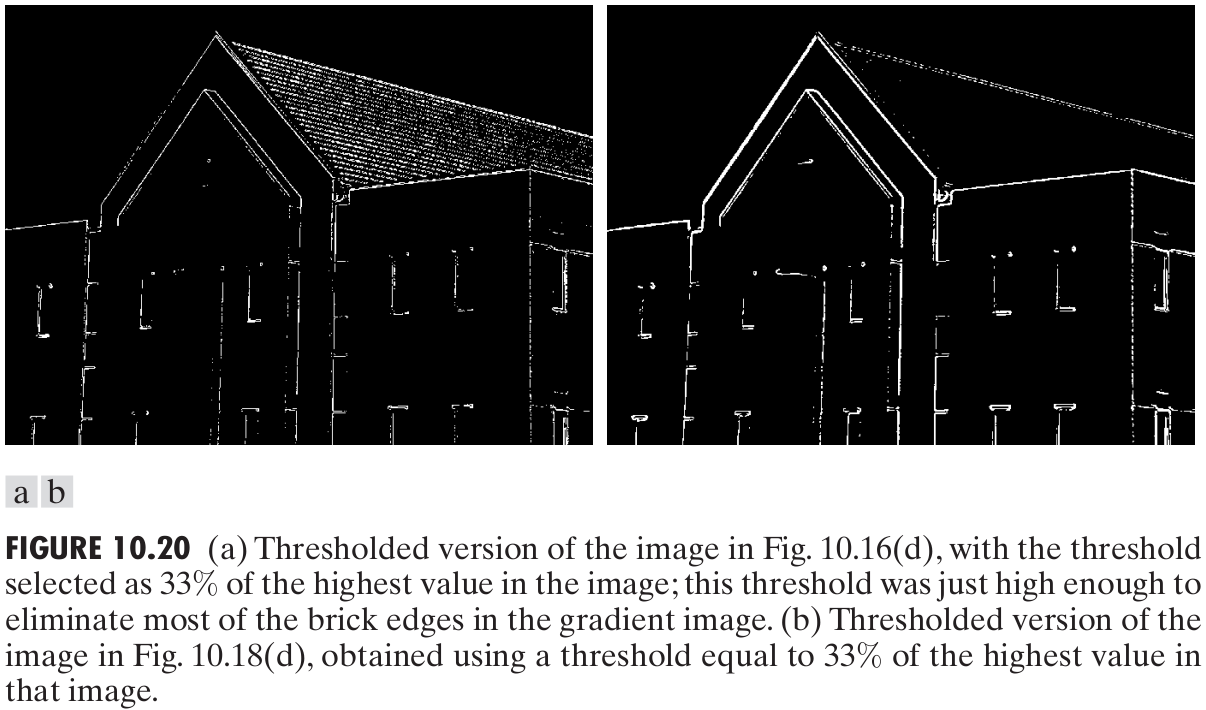
\includegraphics[width=\textwidth]{fig-10-20.png}
\end{figure}
\end{frame}

\subsection{More advanced techniques for edge detection}

\begin{frame}
%\frametitle{More advanced techniques for edge detection}
\begin{itemize}
\item We've seen edge detection through filtering regardless of edge characteristics and noise content.
\item Let's learn more advanced techniques aimed at tackling noise and edge natures.
\end{itemize}
\end{frame}

\subsubsection{The Marr-Hildreth edge detector}

\begin{frame}
%\frametitle{The Marr-Hildreth edge detector}
Marr and Hildreth argued that:
\begin{enumerate}
\item Intensity changes depend on image scale. Hence we must use operators of different sizes.
\item Sudden intensity change will give rise to a peak in the 1st derivative (or, equivalently, to a zero-crossing in the 2nd derivative).
\end{enumerate}
%\frametitle{The Marr-Hildreth edge detector}
Hence, an operator should;
\begin{enumerate}
\item be a differential operator for computing the first or second derivative.
\item be adjustable for different scales (blurred and sharp edges).
\end{enumerate}
\end{frame}

\begin{frame}
%\frametitle{The Marr-Hildreth edge detector}
They argued that the best operator is the Laplacian-of-Gaussian $\nabla^{2}G(x,y)$, where
\[
G(x,y) = e^{-\dfrac{x^{2}+y^{2}}{2\sigma^{2}}}.
\]
\[
\nabla^{2} G(x,y) = \left ( \dfrac{x^{2}+y^{2}-2\sigma^{2}}{\sigma^{4}} \right ) e^{-\dfrac{x^{2}+y^{2}}{2\sigma^{2}}}
\]
\end{frame}

\begin{frame}
%\frametitle{The Marr-Hildreth edge detector}
\begin{figure}[!h]
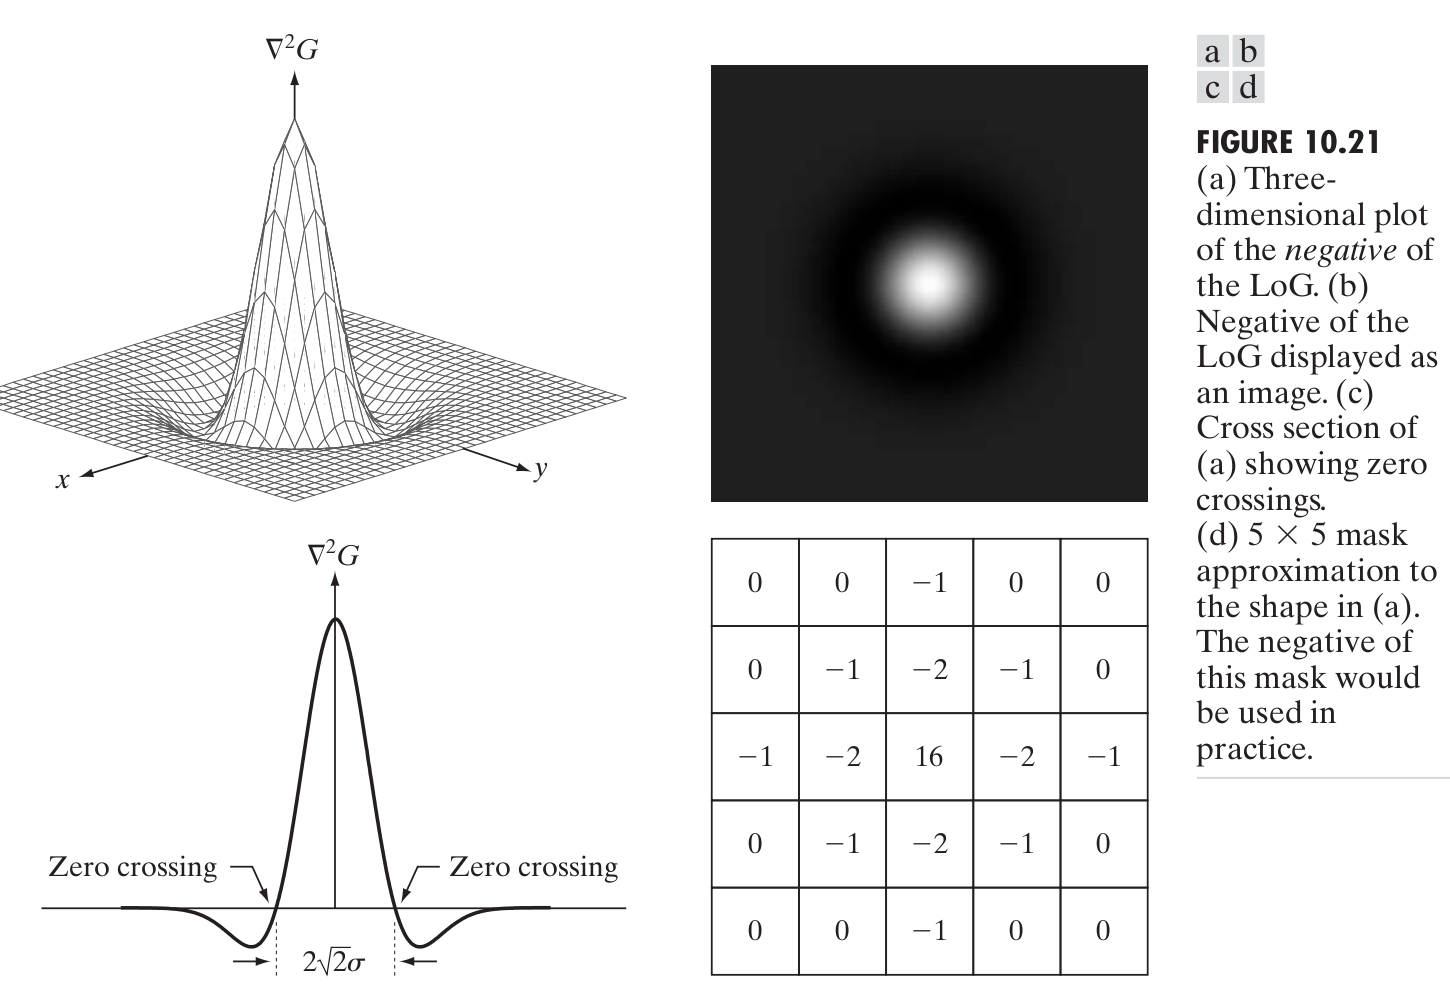
\includegraphics[width=\textwidth]{fig-10-21.png}
\end{figure}
\end{frame}

\begin{frame}
%\frametitle{The Marr-Hildreth edge detector}
Two fundamental ideas:
\begin{enumerate}
\item Reduce details much smaller than $\sigma$ by blurring the image with a Gaussian.
\item Detect abrupt changes through the Laplacian (which is isotropic).
\end{enumerate}
\end{frame}

\begin{frame}
%\frametitle{The Marr-Hildreth edge detector}
The algorithm relies on the Laplacian-of-Gaussian (LoG) operator:
$
g(x,y) = \left [ \nabla^{2} G(x,y) \right ] \star f(x,y) = \nabla^{2} \left [ G(x,y) \star f(x,y) \right ]
$
\begin{block}{The Marr-Hildreth algorithm}
\begin{enumerate}
\item Filter the input image $f(x,y)$ with an $n\times n$ Guassian lowpass filter\footnote{Choose $n$ as the smallest integer greater than $6\sigma$ (since 99.7\% of the Guassian volume lies within $\pm 3\sigma$)}.
\item Compute the Laplacian of the filtered image.
\item Find zero-crossings of the result.
\end{enumerate}
\end{block}
\end{frame}

\begin{frame}
%\frametitle{The Marr-Hildreth edge detector}
\begin{figure}[!h]
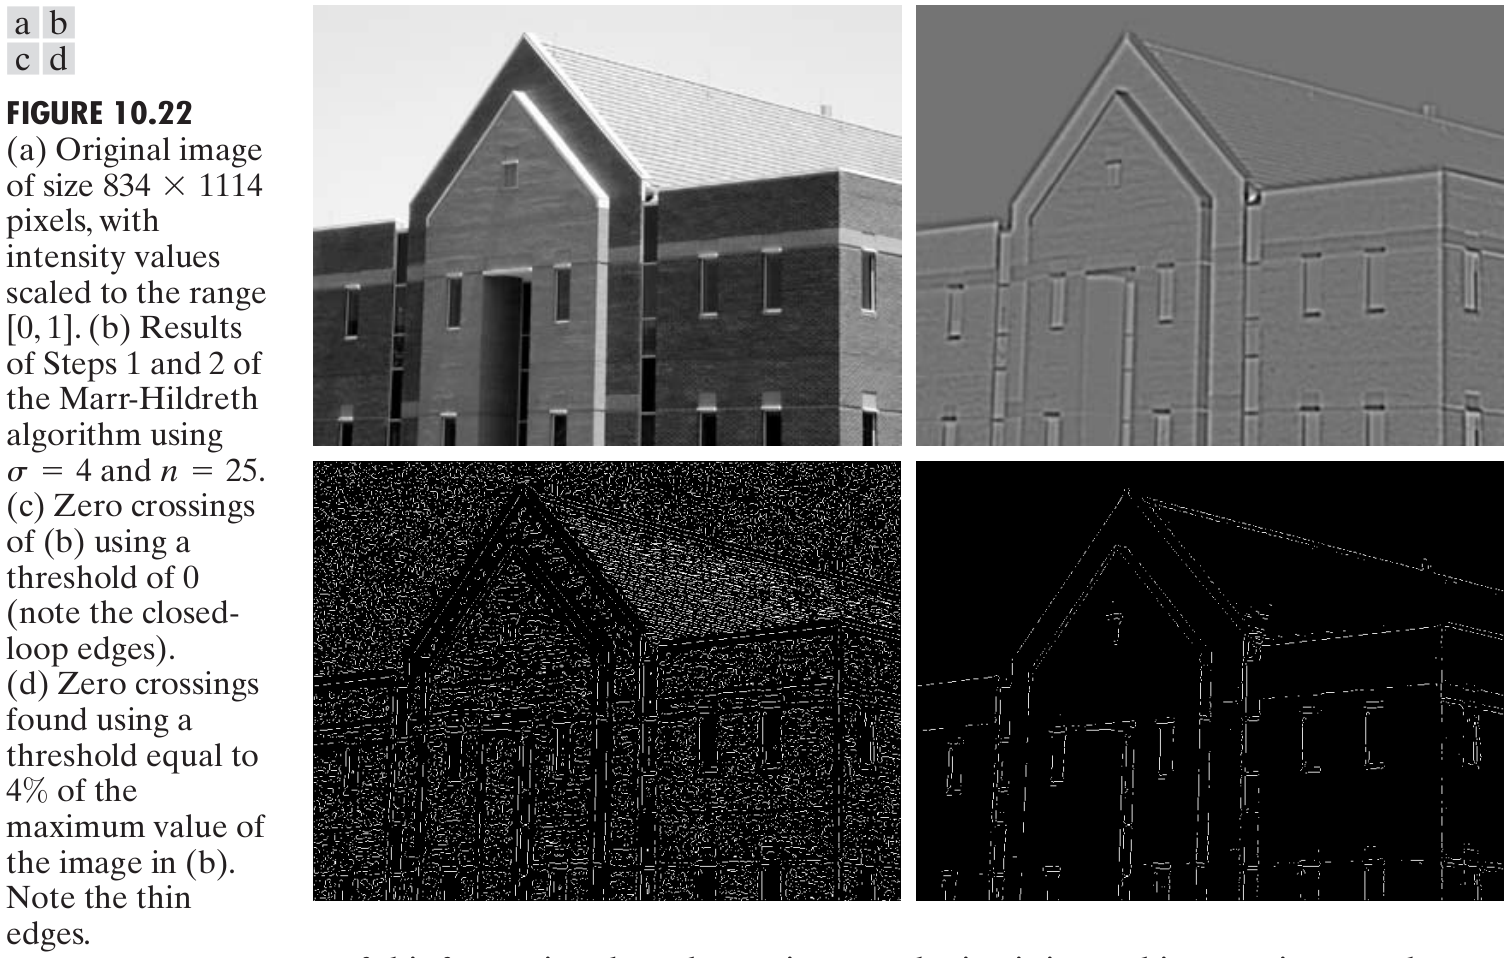
\includegraphics[width=\textwidth]{fig-10-22}
\end{figure}
\end{frame}

\subsubsection{The Canny edge detector}

\begin{frame}
%\frametitle{The Canny edge detector}
\begin{itemize}
\item The Canny edge detector is more complex but better.
\item Three main objectives:
\begin{enumerate}
\item Low error rate:
\begin{itemize}
\item All edges should be found (low false negative).
\item There should be no spurious responses (low false positive).
\end{itemize}
\item Edge points should be well localized.
\item Single edge point response (minimum number of local maxima around the true edge).
\end{enumerate}
\end{itemize}
\end{frame}

\begin{frame}
%\frametitle{The Canny edge detector}
Overview of the Canny edge detector:
\begin{enumerate}
\item Smooth the input image with a Gaussian filter
\item Compute the gradient magnitude and angle images.
\item Apply non-maxima suppression to the gradient magnitude image.
\item Use double thresholding and connectivity analysis to detect and link edges.
\end{enumerate}
\end{frame}

\begin{frame}
%\frametitle{The Canny edge detector}
To meet these three criteria, Canny used;
\begin{enumerate}
\item numerical optimization;
\item 1-D step edges;
\item corruption by additive white Gaussian noise;
\end{enumerate}
%
To find the optimal edge detector:
\[
\dfrac{d}{dx}e^{-\dfrac{x^{2}}{2\sigma^{2}}} = -\dfrac{x}{\sigma^2} e ^{-\dfrac{x^{2}}{2\sigma^{2}}}.
\]
\end{frame}

\begin{frame}
%\frametitle{The Canny edge detector}
Generalizing to 2-D:
\[
G(x,y) = e^{-\dfrac{x^{2}+y^{2}}{2\sigma^{2}}}.
\]
\[
f_{s} = G(x,y) \star f(x,y).
\]
Then we compute the gradient magnitude and direction:
\[
M(x,y) = \sqrt{ g_{x}^{2} + g_{y}^{2} },
\]
\[
\alpha(x,y) = \tan^{-1}(g_{y}/g_{x}).
\]
where $g_{x} = \partial f / \partial x$ and $g_{y} = \partial f / \partial y$.
\end{frame}

\begin{frame}
%\frametitle{The Canny edge detector}
\begin{itemize}
\item Next step: thin wide ridges resulting from the gradient operation (first derivatives are constant throughout edge limits).
\item Use \textit{nonmaxima suppression}.
\end{itemize}
\end{frame}

\begin{frame}
%\frametitle{The Canny edge detector}
Nonmaxima suppression; analyze neighborhood around each point of $\alpha(x,y)$:
\begin{enumerate}
\item Find direction $d_{k}$ closest to $\alpha(x,y)$.
\item If $M(x,y)$ is less than at least one of its two neighbors along $d_{k}$, let $g_{N}(x,y)=0$ (suppression), otherwise, $g_{N}(x,y) = M(x,y)$.
\end{enumerate}
Image $g_{N}$:
\begin{itemize}
\item Is the non-maxima suppressed image.
\item Contains only the thinned edges; it is equal to $M(x,y)$ with the non-maxima edge points suppressed.
\end{itemize}
\end{frame}

\begin{frame}
%\frametitle{The Canny edge detector}
Nonmaxima suppression; analyze neighborhood around each point of $\alpha(x,y)$:
\begin{figure}[!h]
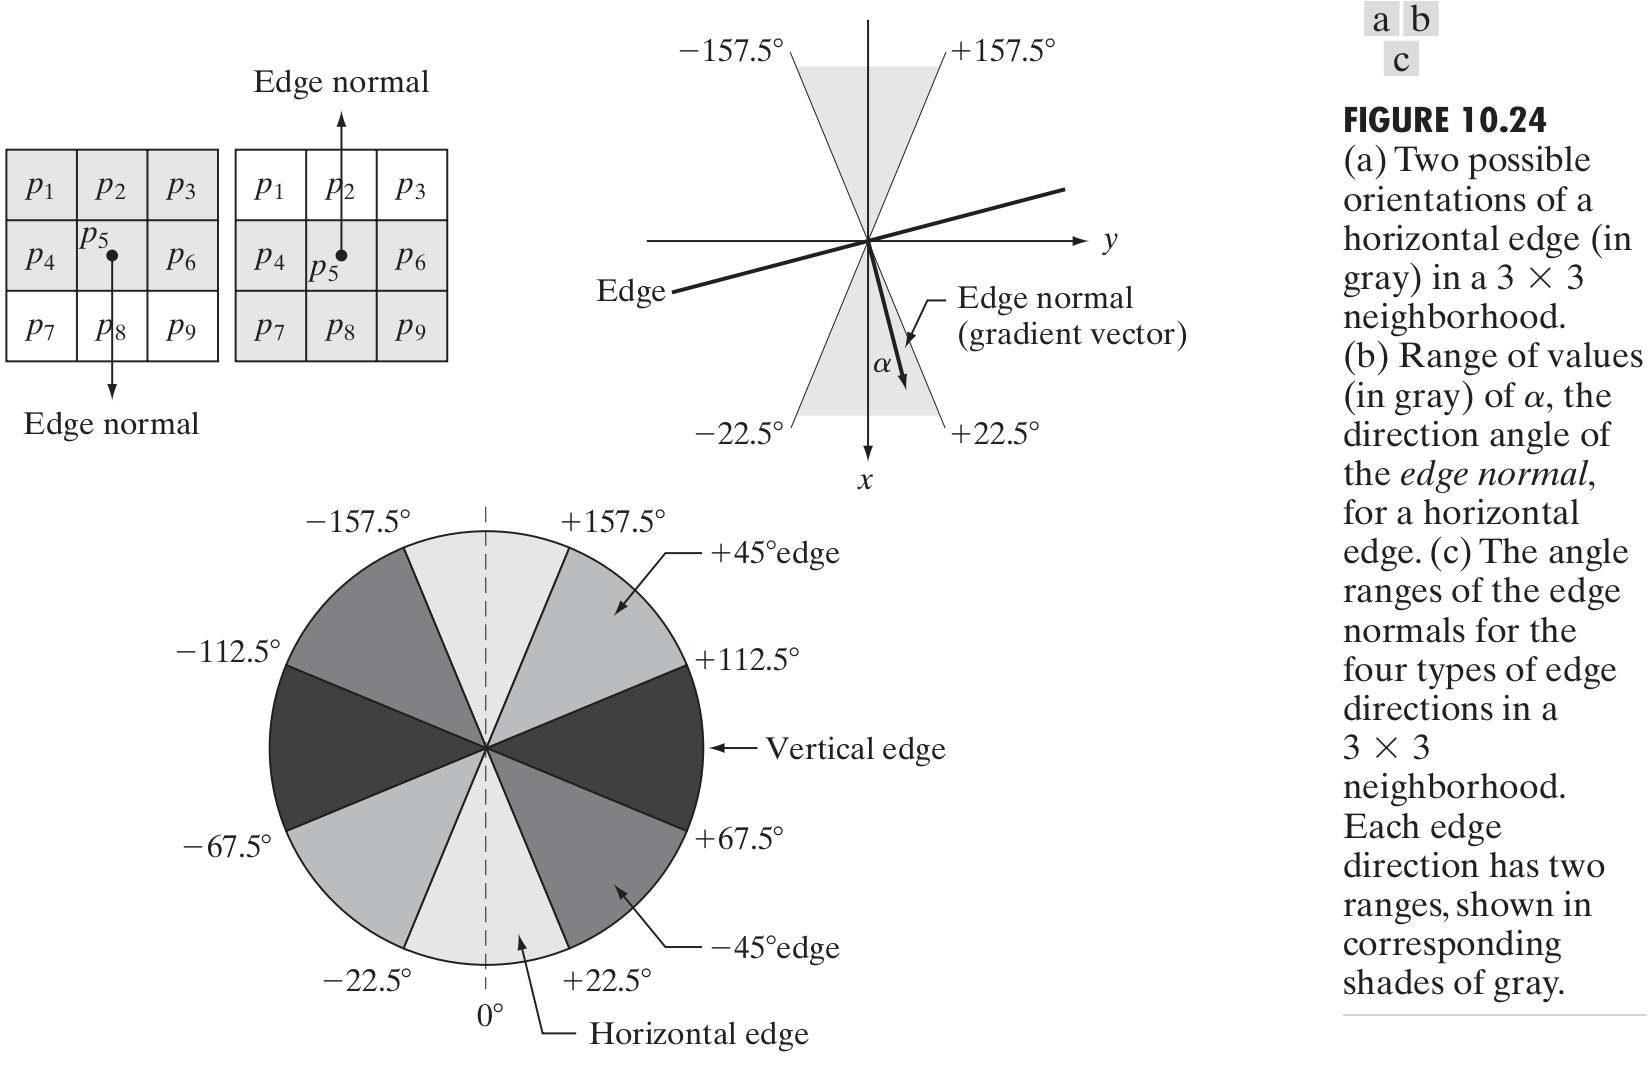
\includegraphics[width=.85\textwidth]{fig-10-24.png}
\end{figure}
\end{frame}

\begin{frame}
%\frametitle{The Canny edge detector}
Next step: thresholding.\\
Initially, $g_{NH}(x,y)$ and $g_{NL}(x,y)$ are set to $0$.
Find:
\begin{itemize}
\item ``Strong'' edges using $g_{NH}(x,y) = g_{N}(x,y) \geq T_{H}$.
\item ``Weak'' edges using $g_{NL}(x,y) = g_{N}(x,y) \geq T_{L}$.
\end{itemize}
Then:
\begin{itemize}
\item Pixels in $g_{NH}$ (typically unconnected) are marked as edge pixels.
\end{itemize}
\end{frame}

\begin{frame}
%\frametitle{The Canny edge detector}
%\begin{columns}
%\begin{column}{.7\textwidth}
\begin{enumerate}
\item Take $p \in g_{NH}(x,y)$.
\item Mark as valid edge pixels all the weak pixels in $g_{NL}$ connected to $p$ (e.g., 8 connectivity).
\item If all nonzero pixels in $g_{NH}(x,y)$ were analyzed go to 4. Else, return to 1.
\item Set to zero all pixels in $g_{NL}(x,y)$ that were not marked as valid edge pixels.
\end{enumerate}
%\end{column}
%\begin{column}{.3\textwidth}
\begin{figure}[!h]
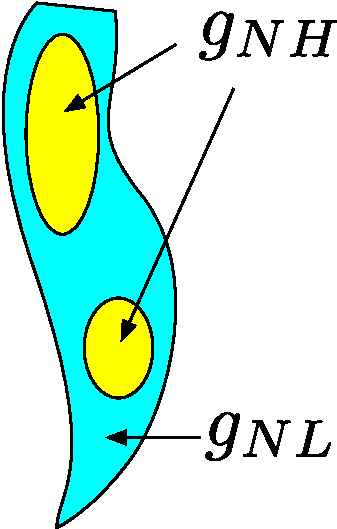
\includegraphics[width=.2\textwidth]{gnh_gnl.pdf}
\end{figure}
%\end{column}
%\end{columns}
In the end, append to $g_{NH}(x,y)$ all nonzero pixels from $g_{NL}$.
\end{frame}

\begin{frame}
%\frametitle{The Canny edge detector}
\begin{figure}[!h]
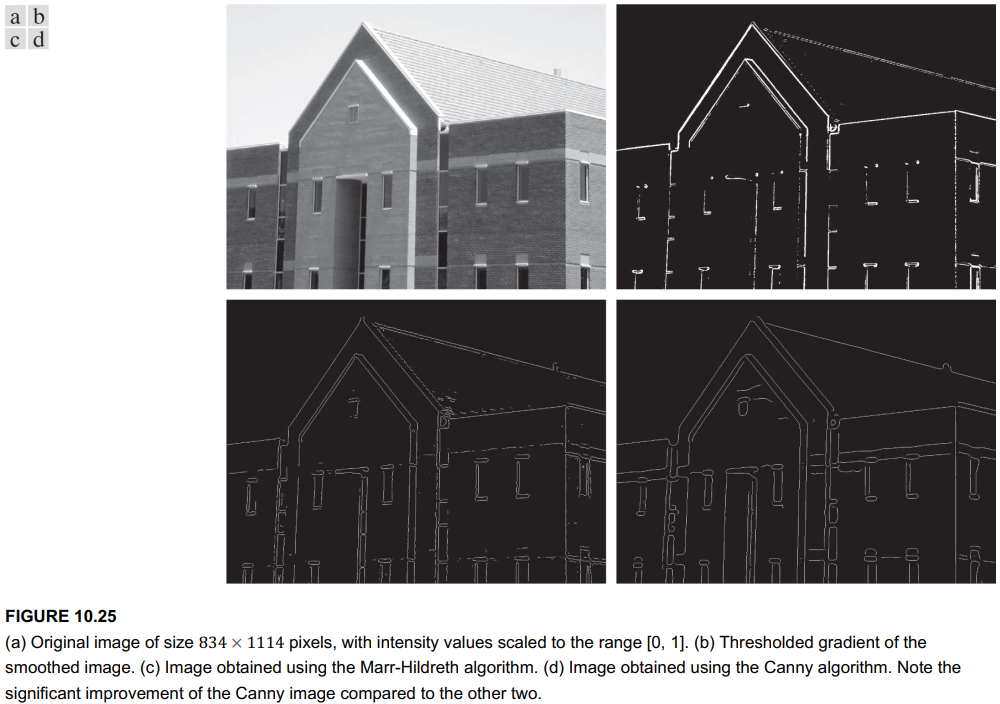
\includegraphics[width=.9\textwidth]{fig-10-25.png}
\end{figure}
\end{frame}

\begin{frame}
%\frametitle{The Canny edge detector}
\begin{figure}[!h]
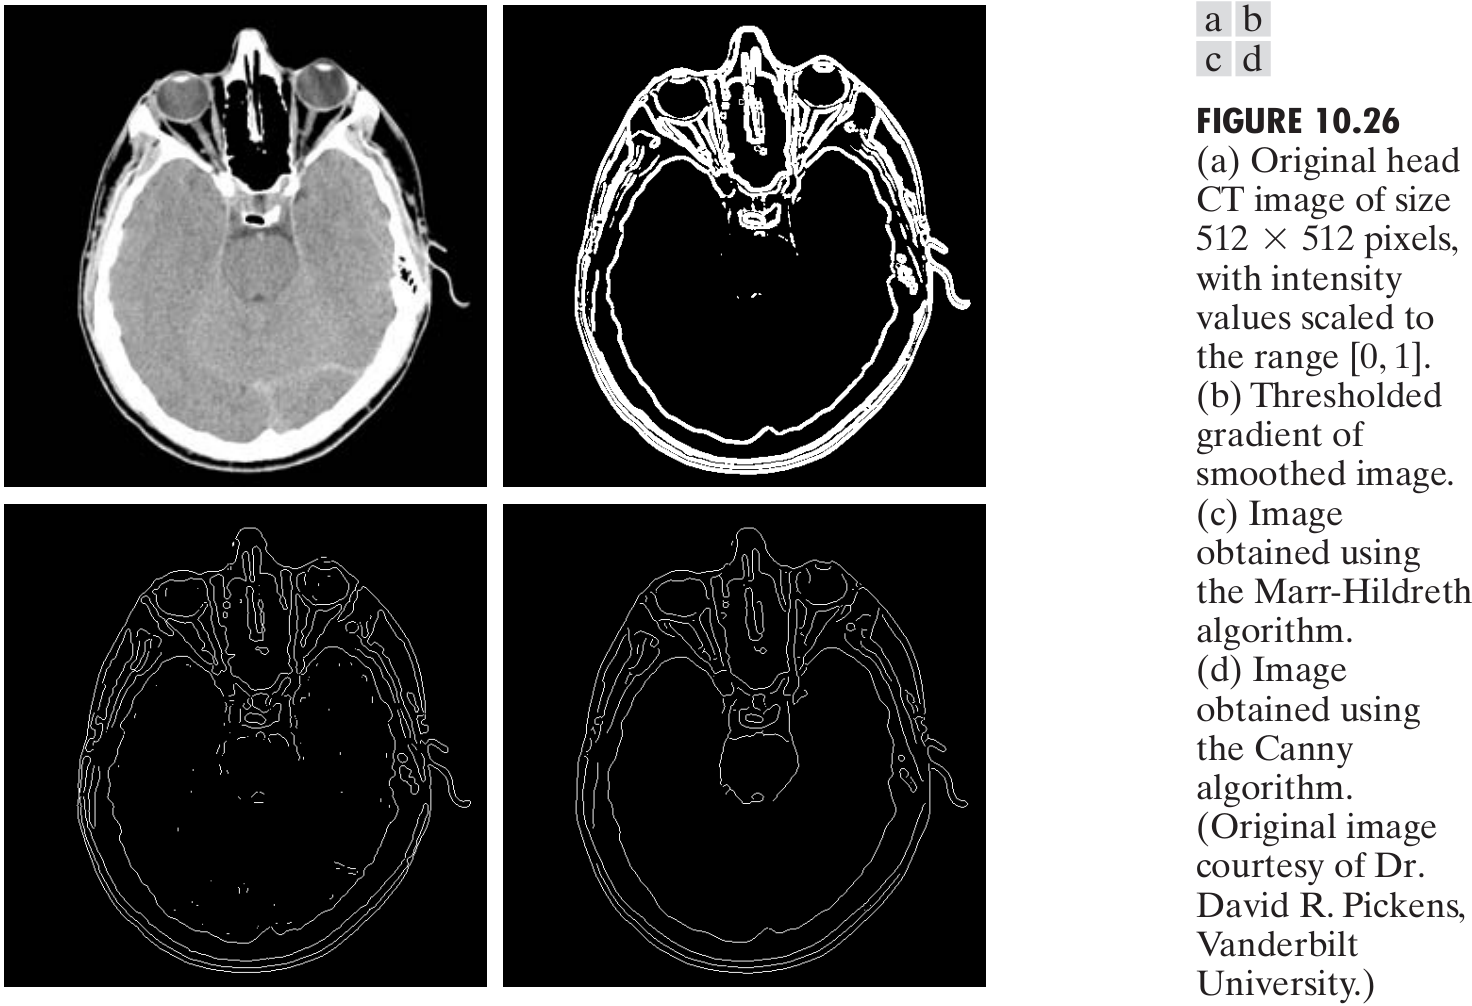
\includegraphics[width=.9\textwidth]{fig-10-26.png}
\end{figure}
\end{frame}

\subsection{Edge linking and boundary detection}

\subsubsection{Global processing using the Hough transform}

\begin{frame}
%\frametitle{Global processing using the Hough transform}
The Hough transform:
\begin{itemize}
\item Developed by Paul Hough in 1962.
\item Can be applied to detect curves that:
\begin{itemize}
\item can be described as a mathematical expression, and;
\item have no constrain in their location.
\end{itemize}
\item Advantage:
\begin{itemize}
\item Relatively insensitive to gaps and noise.
\end{itemize}
\end{itemize}
\end{frame}

\begin{frame}
%\frametitle{Global processing using the Hough transform}
\begin{itemize}
\item Consider point $p_{i} = (x_{i}, y_{i})$ in plane $S_{xy}$.
\item Infinitely many lines pass through $p_{i}$ for varying values of $a$ and $b$ satisfying $y_{i} = ax_{i} + b$.
\item In plane $S_{ab}$, point $p_{i}$ is transformed into line $b = -x_{i}a+y_{i}$.
\item Equivalently, point $p_{j}$ is transformed into line $b = -x_{j}a + y_{j}$.
\end{itemize}
\begin{figure}[!h]
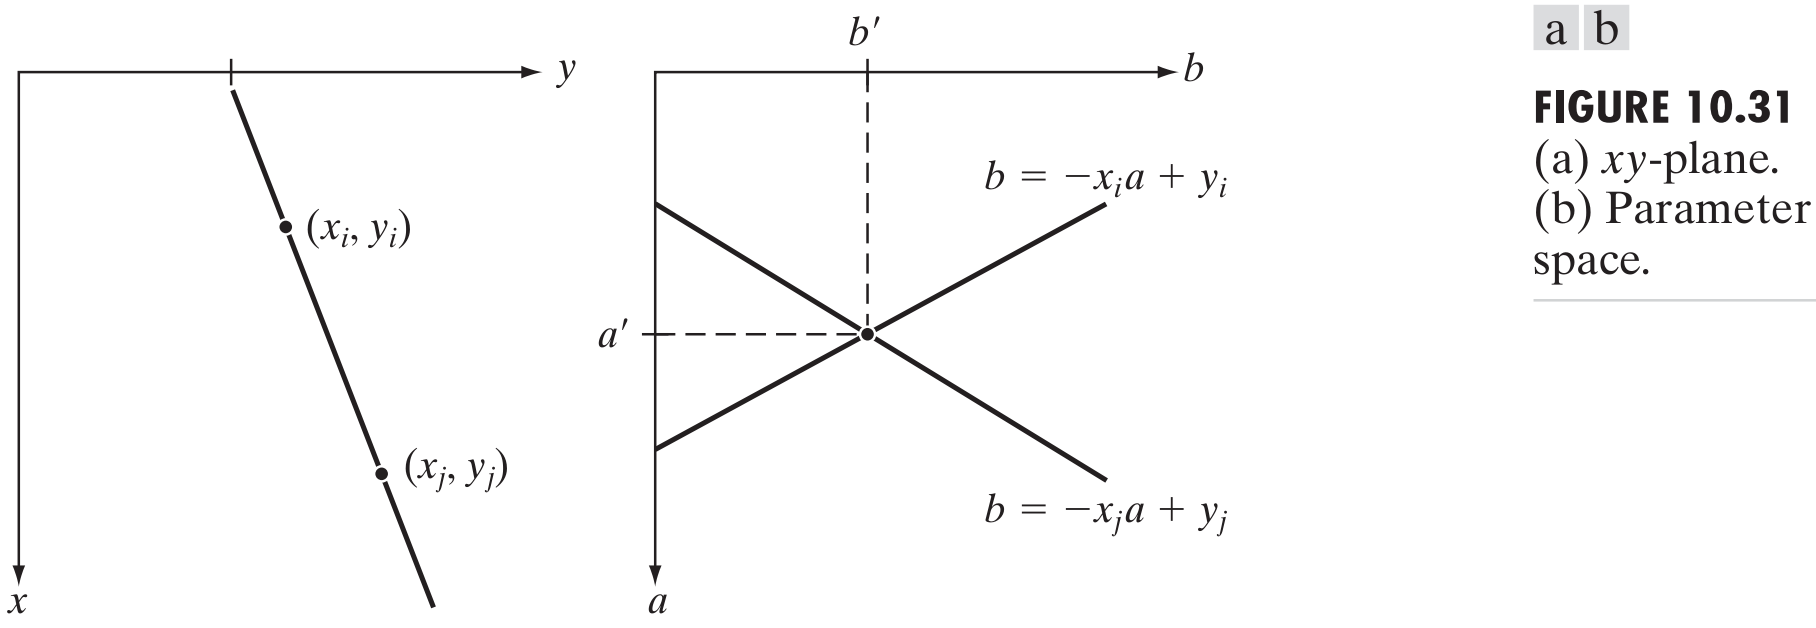
\includegraphics[width=.8\textwidth]{fig-10-31.png}
\end{figure}
\end{frame}

\begin{frame}
%\frametitle{Global processing using the Hough transform}
\begin{itemize}
\item A line in $S_{xy}$ is transformed into a point in $S_{ab}$ and vice-versa.
\item Points $p_{i}$ and $p_{j}$ lie on the line given by equation $y = a'x + b'$.
\item All points lying on this line on $S_{xy}$ are transformed into lines in $S_{ab}$ that intersect at point $(a', b')$.
\item The higher the number of points, the more lines intersect.
\end{itemize}
\begin{figure}[!h]
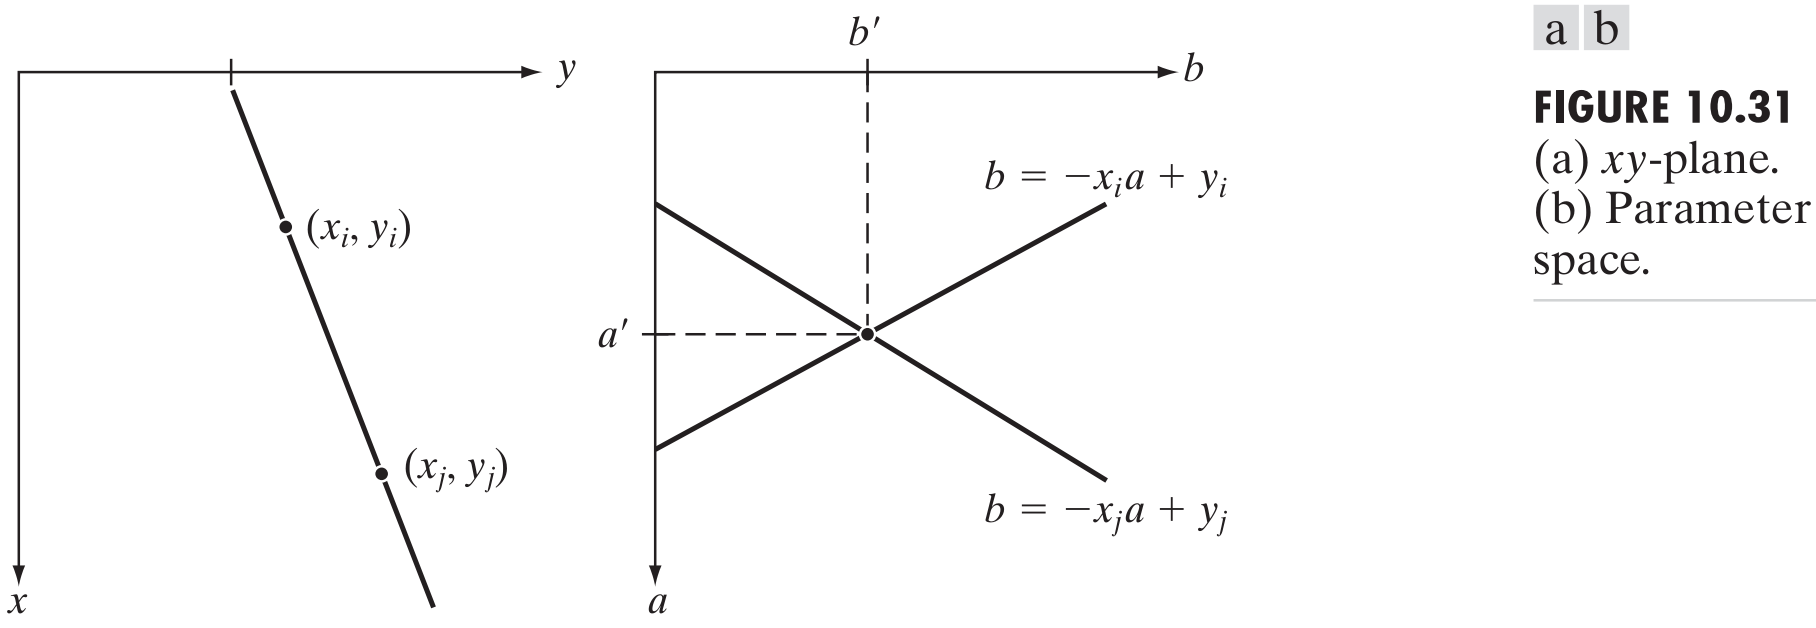
\includegraphics[width=.8\textwidth]{fig-10-31.png}
\end{figure}
\end{frame}

\begin{frame}
%\frametitle{Global processing using the Hough transform}
\begin{itemize}
\item The number of lines intersecting at $(a',b')$ in $S_{ab}$ denote the number of points in $S_{xy}$ belonging to line $y = a'x + b'$.
\item We can find dense lines in $S_{xy}$ by finding points in $S_{ab} $ where several lines intersect.
\end{itemize}
\begin{figure}[!h]
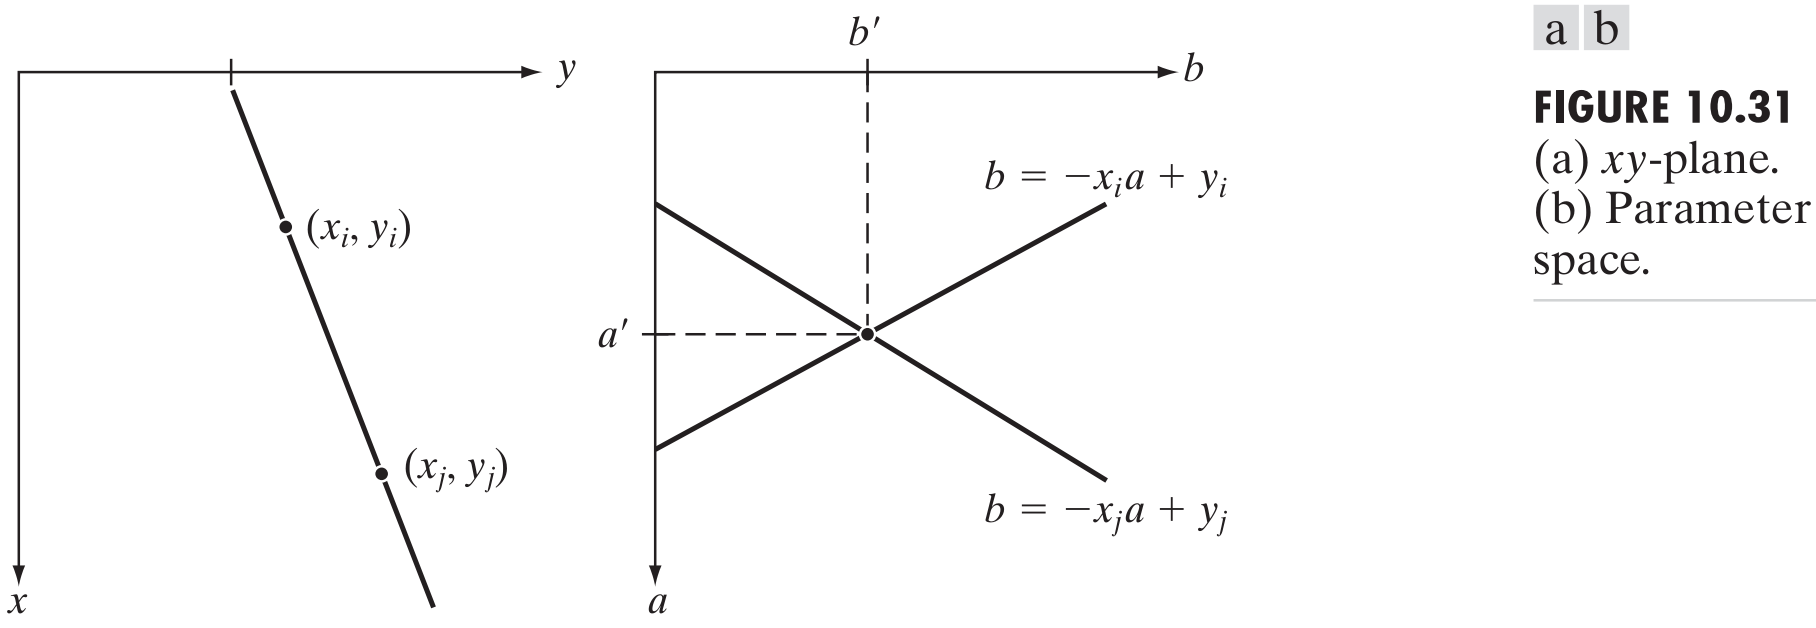
\includegraphics[width=.8\textwidth]{fig-10-31.png}
\end{figure}
\end{frame}

\begin{frame}
%\frametitle{Global processing using the Hough transform}
\begin{itemize}
\item One problem! With vertical lines: $b \mapsto \infty$.
\item The solution is to use:
\begin{equation}
x\cos\theta + y\sin\theta = \rho.
\end{equation}
\item In this case, points in $S_{xy}$ map to sinusoids in $S_{ab}$.
\end{itemize}
\begin{figure}[!h]
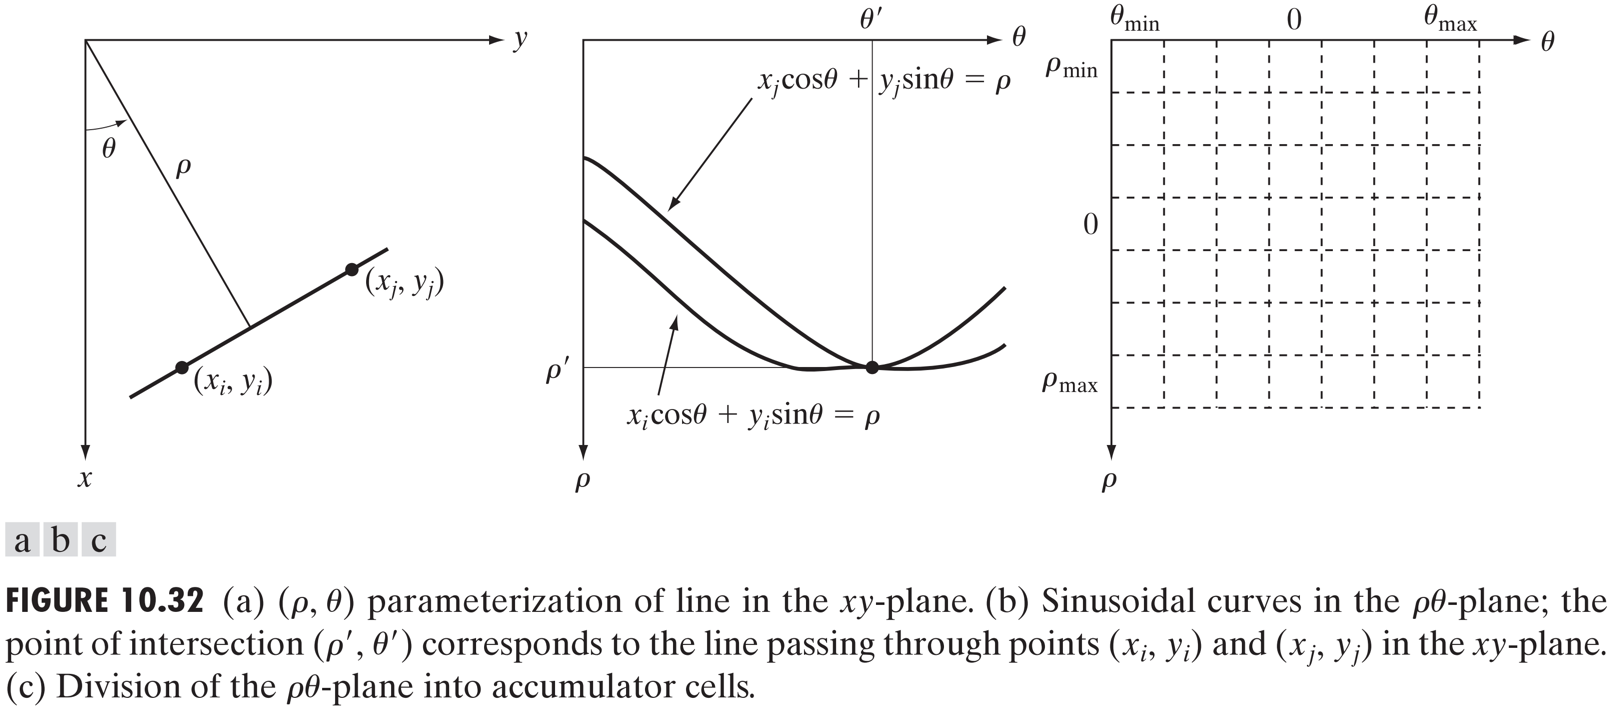
\includegraphics[width=.8\textwidth]{fig-10-32.png}
\end{figure}
\end{frame}

\begin{frame}
%\frametitle{Global processing using the Hough transform}
\begin{figure}[!h]
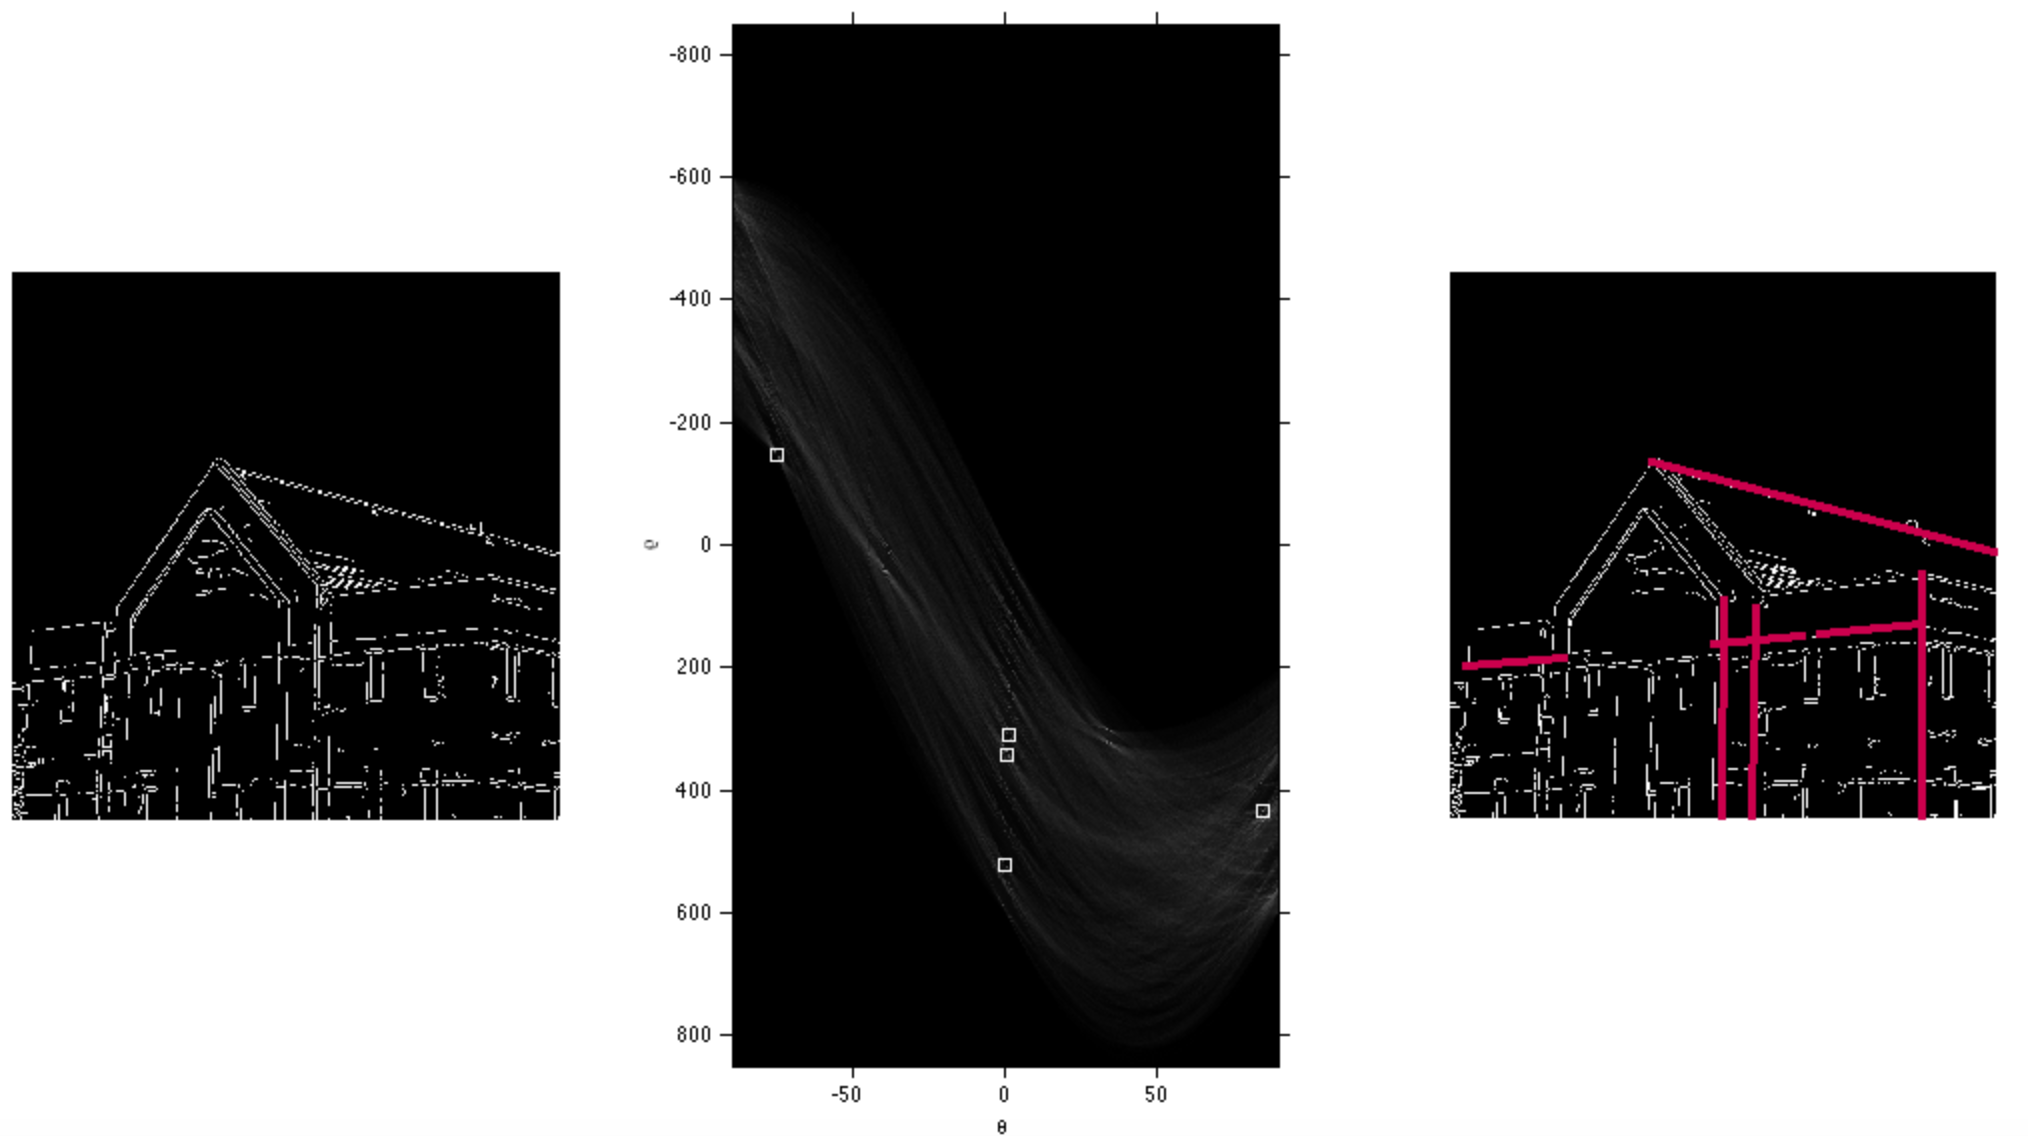
\includegraphics[width=\textwidth]{ex-11-6.png}
\end{figure}
\end{frame}

%\section{Detection of similarities}

\section{Thresholding}

\subsection{Foundation}

\begin{frame}
%\frametitle{Thresholding}
\begin{itemize}
\item A grayscale image $f(x,y)$ can be divided into:
\begin{itemize}
\item Background.
\item Foreground.
\end{itemize}
\item Threshold ($T$) is a grayscale level capable of performing the separation:
\[
g(x,y) = \left \{
\begin{array}{ll}
1 & \text{if } f(x,y) > T \\
0 & \text{if } f(x,y) \leq T
\end{array}
\right ..
\]
\end{itemize}
\begin{figure}[!h]
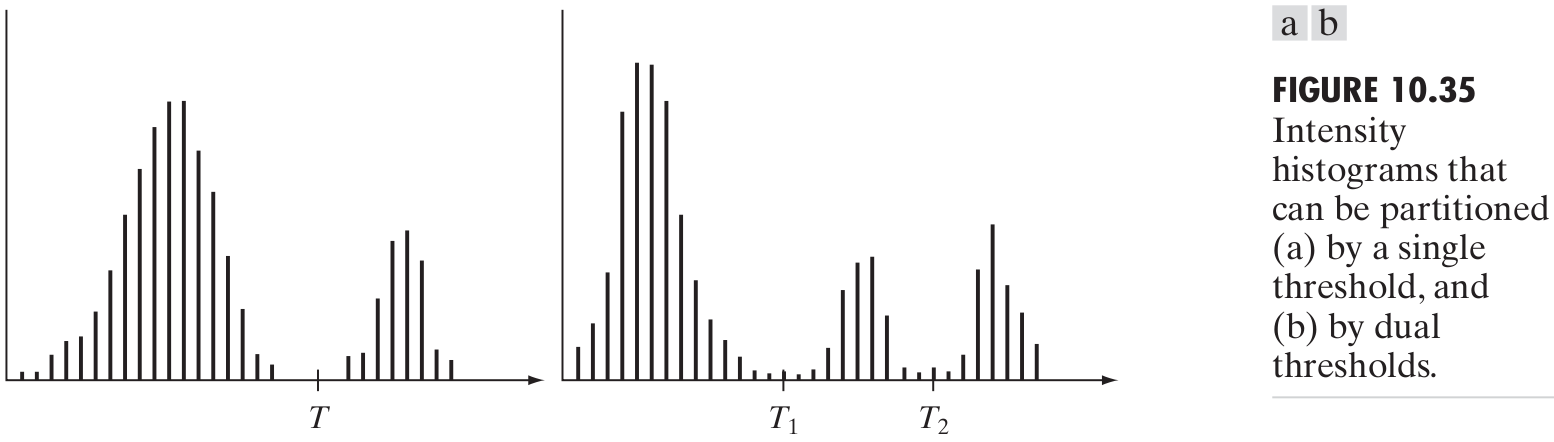
\includegraphics[width=.8\textwidth]{fig-10-35.png}
\end{figure}
\end{frame}


\begin{frame}%{Thresholding}
\begin{itemize}
\item There can be various threshold levels.
\item $T$ can be fixed (\textit{global thresholding}) or not (variable thresholding).
\item $T$ may also depend on the neighborhood of the pixel (adaptive thresholding).
\end{itemize}
\end{frame}

\begin{frame}
%\frametitle{Thresholding}
\[
g(x,y) = \left \{
\begin{array}{ll}
a & \text{if } f(x,y) > T_{2} \\
b & \text{if } T_{1} < f(x,y) \leq T_{2} \\
c & \text{if } f(x,y) \leq T_{1}
\end{array}
\right ..
\]
\begin{figure}[!h]
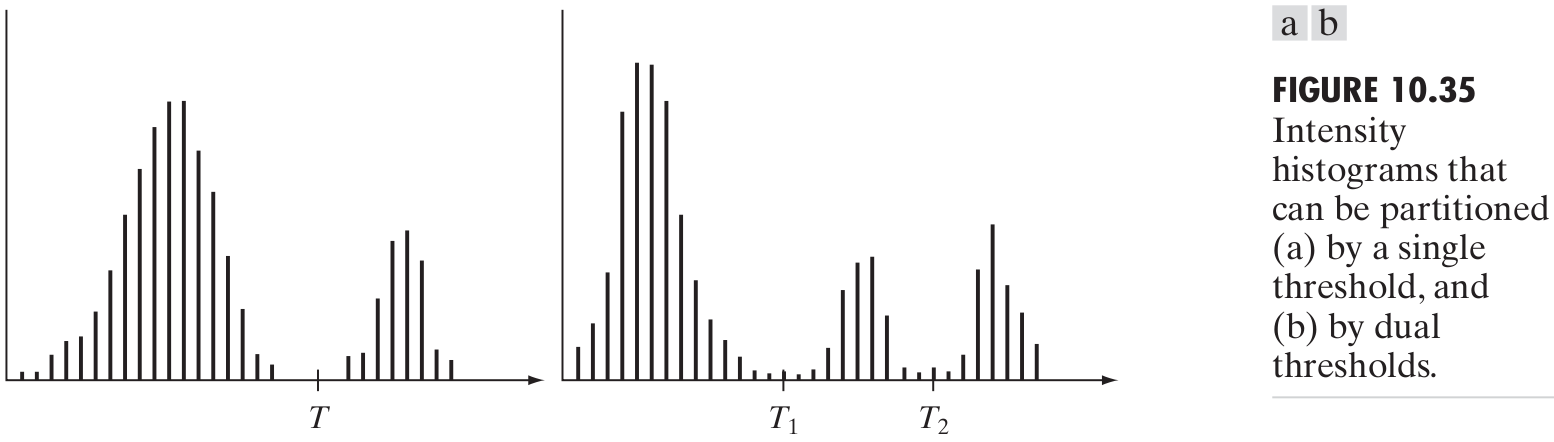
\includegraphics[width=.8\textwidth]{fig-10-35.png}
\end{figure}
\end{frame}

\begin{frame}
%\frametitle{Thresholding}
\begin{itemize}
\item Intensity thresholding depends on width and depth of the valley(s) separating the histogram modes.
\item Key factors affecting the properties of the valley(s):
\begin{enumerate}
\item Separation between peaks.
\item Noise content in the image.
\item Relative sizes of objects and background.
\item Uniformity of the illumination source.
\item Uniformity of the reflectance properties of the image.
\end{enumerate}
\end{itemize}
\end{frame}

\subsubsection{The role of noise in image thresholding}

\begin{frame}
%\frametitle{The role of noise in image thresholding}
Problem 1: noise.
\begin{figure}[!h]
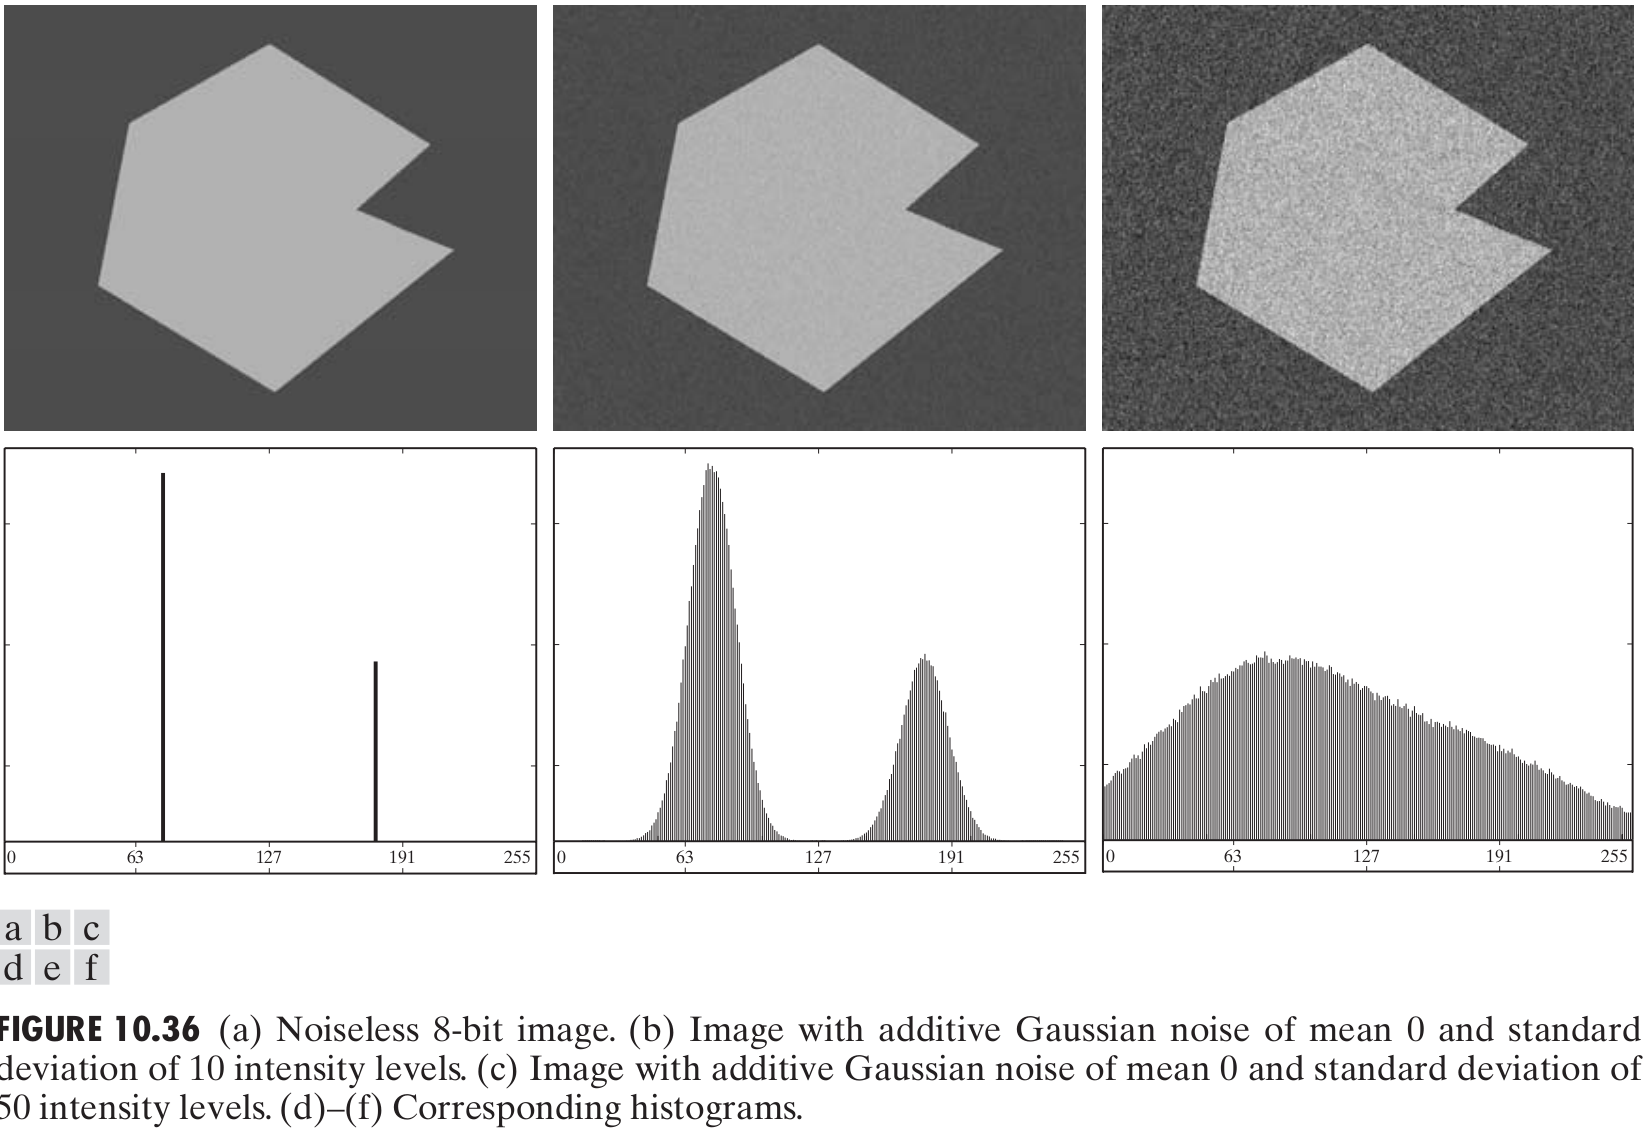
\includegraphics[width=.7\textwidth]{fig-10-36.png}
\end{figure}
\end{frame}

\subsubsection{The role of illumination and reflectance}

\begin{frame}
%\frametitle{The role of illumination and reflectance}
Effect of non-uniform illumination:
\begin{figure}[!h]
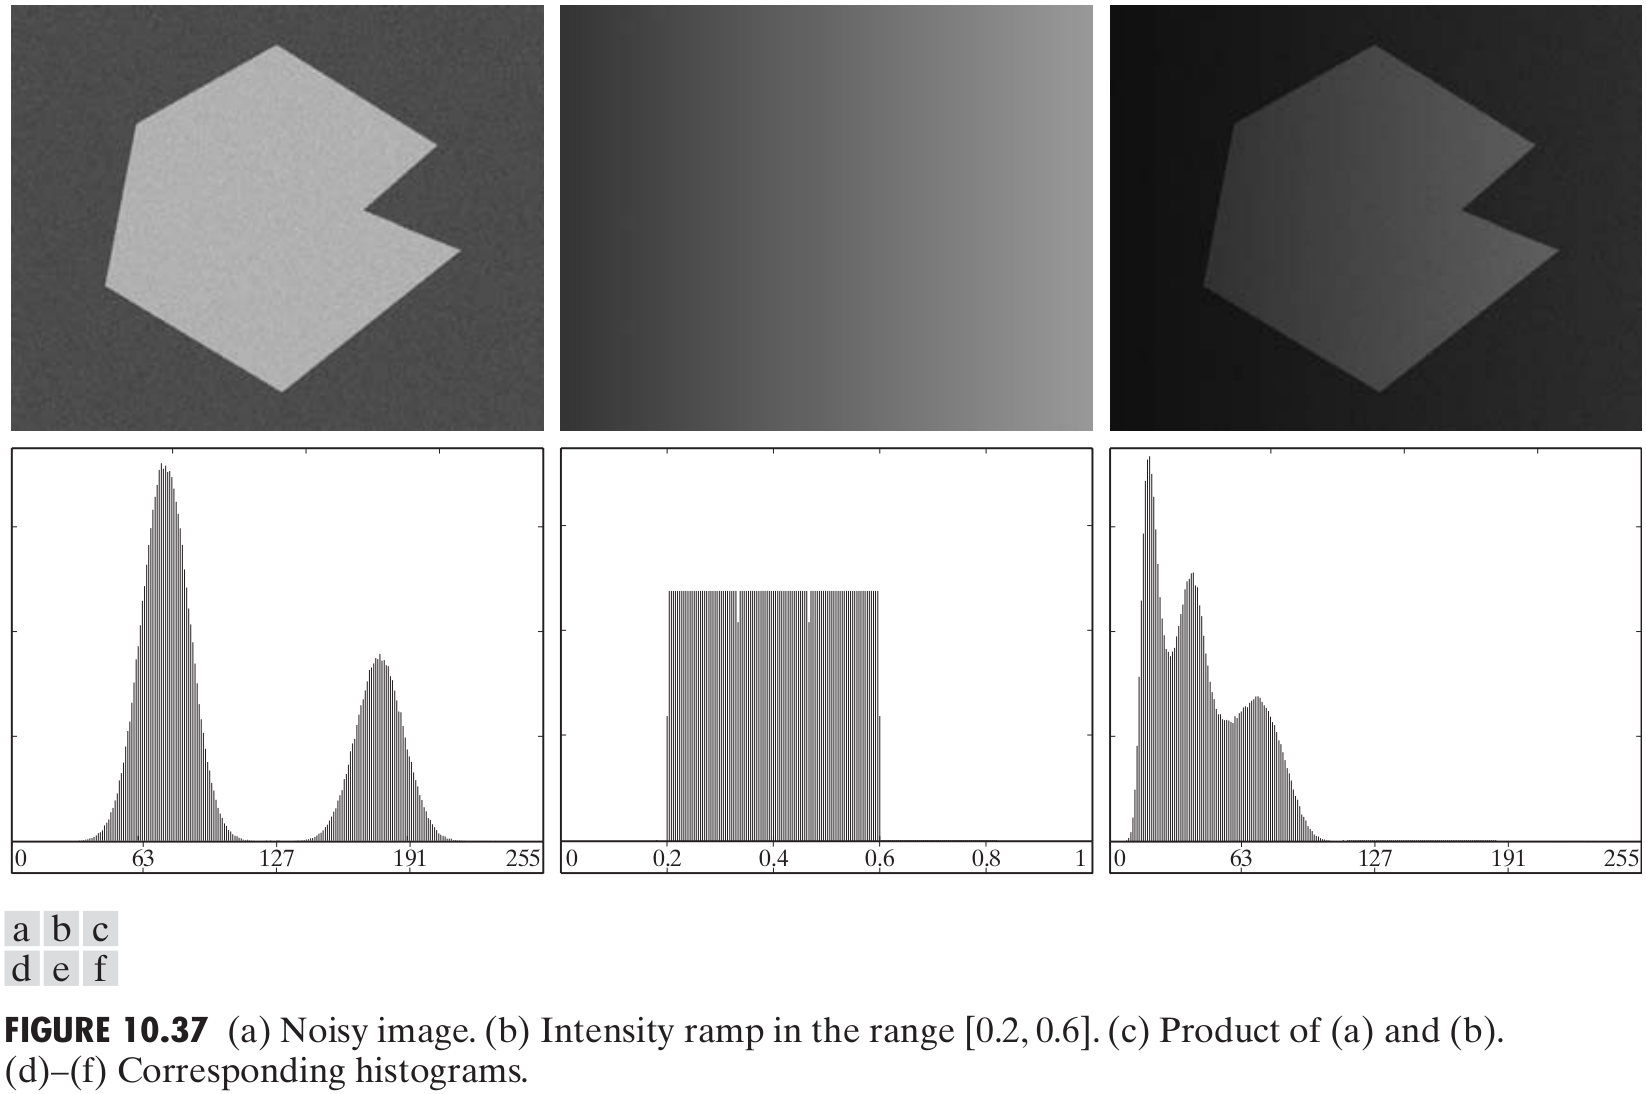
\includegraphics[width=.7\textwidth]{fig-10-37.png}
\end{figure}
\end{frame}

\begin{frame}
%\frametitle{The role of illumination and reflectance}
\begin{block}{Thresholding}
Illumination and reflectance play a central role in the success of image segmentation using thresholding or other segmentation techniques.
\end{block}
\begin{block}{Attention}
If possible, control these problems when facing a segmentation challenge!!!
\end{block}
\begin{itemize}
\item Example: industrial applications.
\end{itemize}
\end{frame}

\begin{frame}
%\frametitle{The role of illumination and reflectance}
Three basic approaches to fix non-uniform illumination and/or object reflectance:
\begin{enumerate}
\item Find the illumination pattern by imaging a flat surface, then multiply its inverse by an input image.
\item Use the top-hat (or bot-hat) transform.
\item Use variable thresholding.
\end{enumerate}
\end{frame}

\subsection{Basic global thresholding}

\begin{frame}
%\frametitle{Basic global thresholding}
\begin{enumerate}
\item Select an initial, $T$, producing $G_{1}$ and $G_{2}$.
\item Compute means $m_{1}$ and $m_{2}$.
\item Update threshold $T = \left (m_{1} + m_{2} \right )/2$.
\item Repeat 2-4 until $T_{i+1}-T_{i} < \delta$.
\end{enumerate}
\begin{figure}[!h]
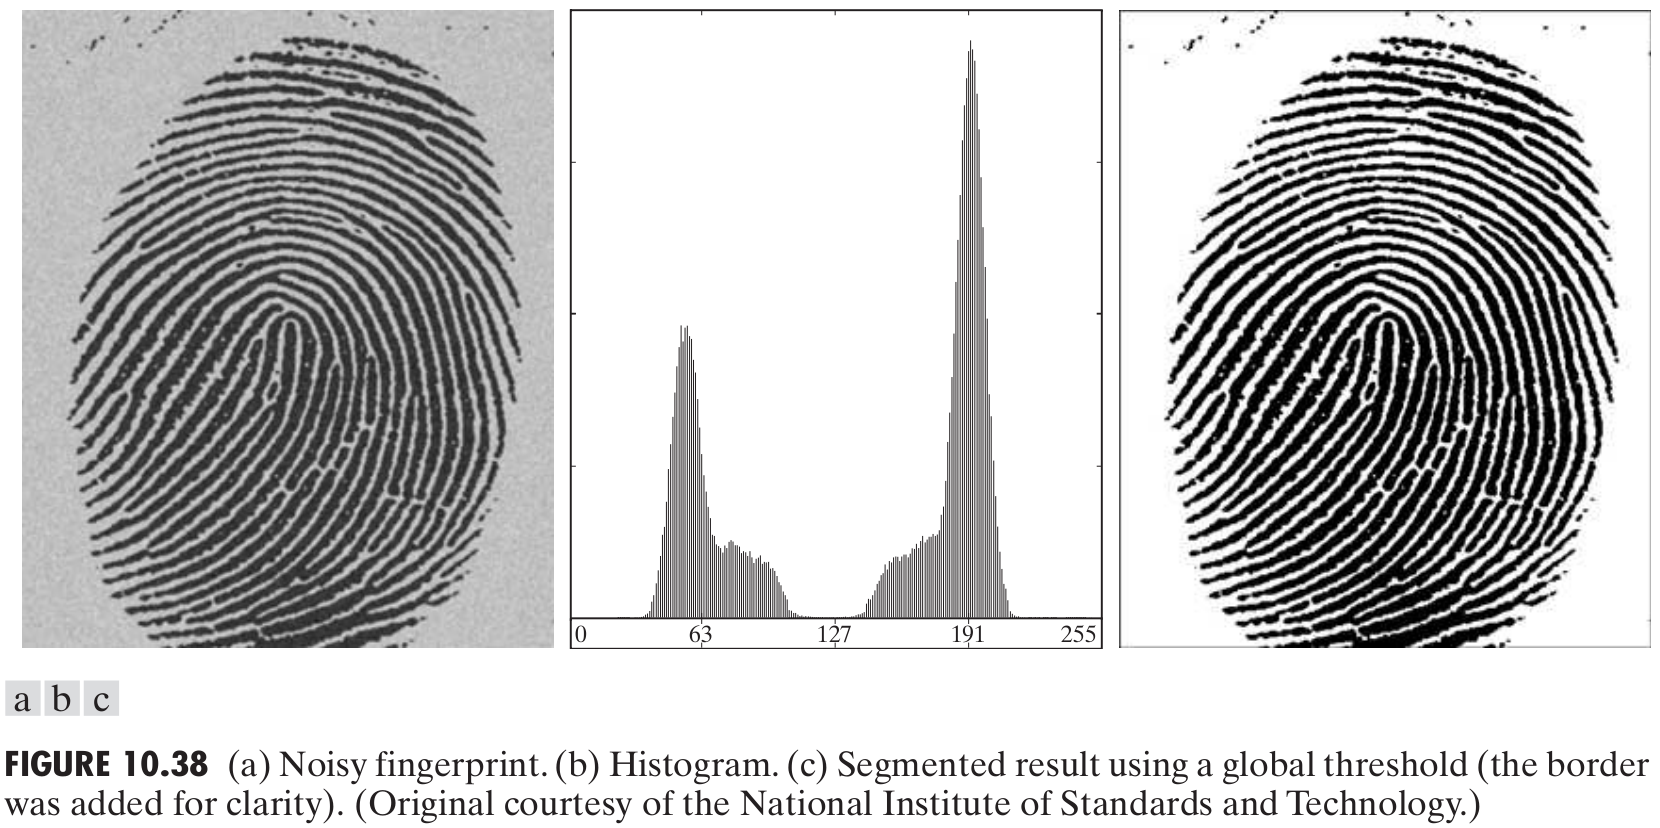
\includegraphics[width=.8\textwidth]{fig-10-38.png}
\end{figure}
\end{frame}

\subsection{Optimum global thresholding using Otsu's method}

\begin{frame}
%\frametitle{Otsu's method}
Suppose we have an image with $N$ pixels, $L$ intensity levels and the following histogram.
\begin{columns}
\begin{column}{.35\textwidth}
\begin{figure}[!h]
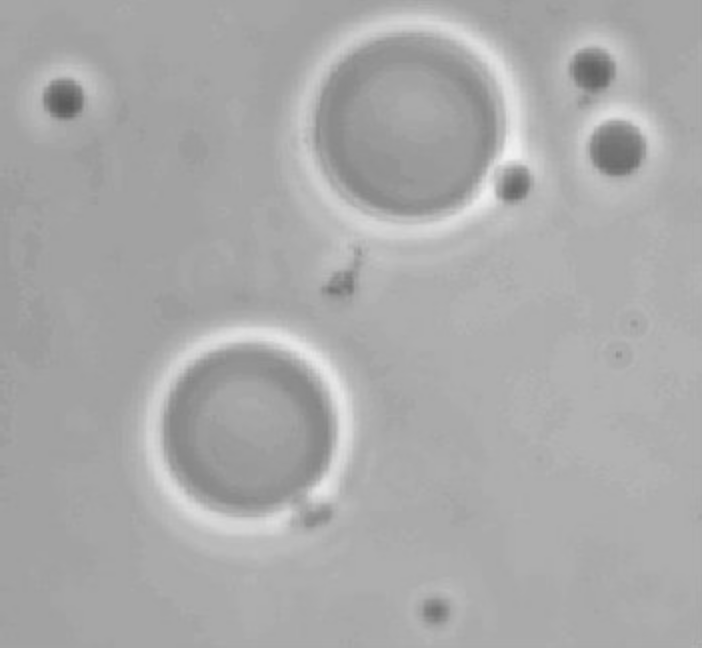
\includegraphics[width=\textwidth]{polymersomes.png}
\end{figure}
\end{column}
\begin{column}{.65\textwidth}
\begin{figure}[!h]
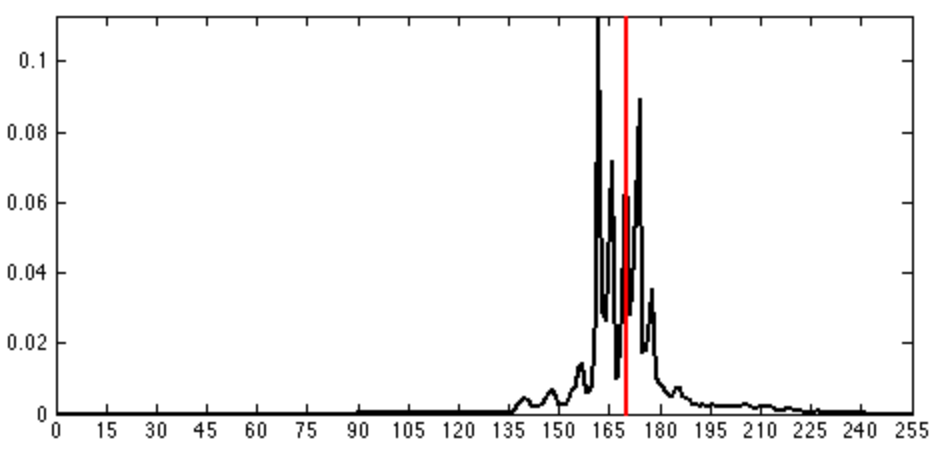
\includegraphics[width=\textwidth]{pdf2.png}
\end{figure}
\end{column}
\end{columns}
\begin{itemize}
\item $n_{i}$ is the number of pixels with intensity $i$.
\item The normalized histogram is such that $\sum_{i=0}^{L-1}p_{i} = 1$, where $p_{i} = n_{i}/N$.
\end{itemize}
\end{frame}

\begin{frame}
%\frametitle{Otsu's method}
\begin{columns}
\begin{column}{.6\textwidth}
\begin{itemize}
\item Segment using a threshold $T$ given by basic global thresholding.
\item The probabilities of labeling a pixel to class $C_{1}$ and $C_{2}$ are
\[
P_{1}(T)=\sum_{i=0}^{T}p_{i}% = \dfrac{1}{N} \sum_{i=0}^{T}n_{i}.
\]
and
\[
P_{2}(T)=\sum_{i=T+1}^{L-1}p_{i} = 1-P_{1}(T).
\]
\end{itemize}
\end{column}
\begin{column}{.4\textwidth}
\begin{figure}[!h]
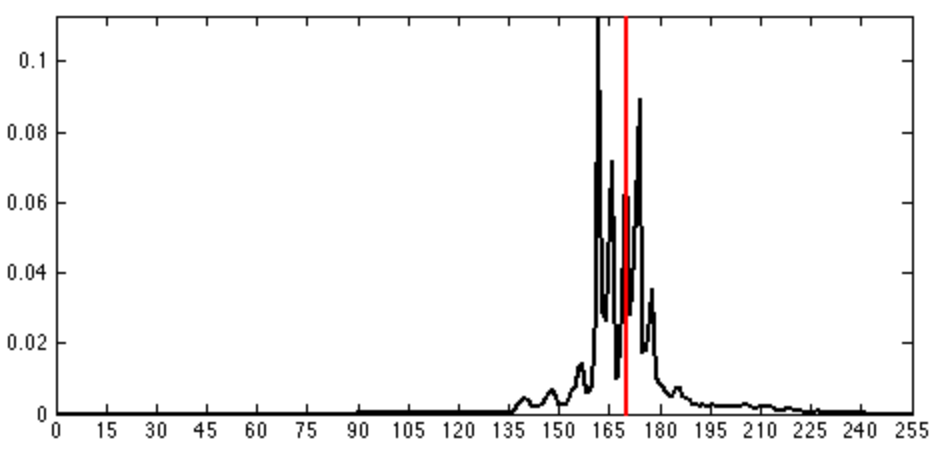
\includegraphics[width=\textwidth]{pdf2.png}
\end{figure}
\begin{figure}[!h]

\includegraphics[width=\textwidth]{polymersomesSeg.png}
\end{figure}
\end{column}
\end{columns}
\end{frame}

\begin{frame}
%\frametitle{Otsu's method}
\begin{itemize}
\item The mean intensity value of the pixels assigned to $C_{1}$ is
$m_{1}(T) = \dfrac{1}{P_{1}(T)} \sum_{i=0}^{T} i p_{i}$.
% \dfrac{\sum_{i=0}^{T} i n_{i}}{\sum_{i=0}^{T}n_{i}} = \dfrac{1}{P_{1}(T)} \dfrac{1}{N} \sum_{i=0}^{T} i n_{i} = 
\item Equivalently...
$m_{2}(T) = \dfrac{1}{P_{2}(T)} \sum_{i=T+1}^{L-1} i p_{i}$.
\end{itemize}
\begin{figure}[!h]
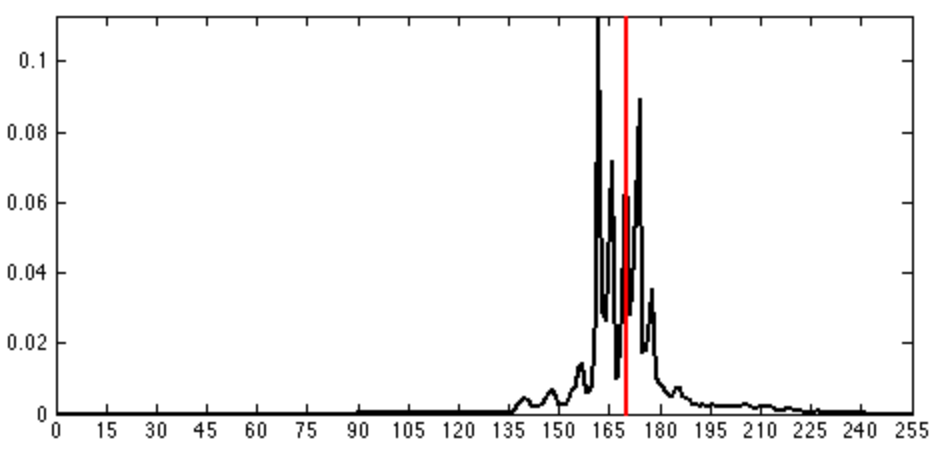
\includegraphics[width=.5\textwidth]{pdf2.png}
\end{figure}
\end{frame}

\begin{frame}
%\frametitle{Otsu's method}
\begin{itemize}
\item The cumulative mean is $m(T) = \sum_{i=0}^{T} ip_{i}$.
\item The global mean is $m_{G}(T) = \sum_{i=0}^{L-1}ip_{i}$.
\item The global variance is  given by
$\sigma_{G}^{2} = \sum_{i=0}^{L-1} (i-m_{G})^{2} p_{i}$.
\item The interclass variance is defined as
$\sigma_{B}^{2}(T) = \left [ P_{1}(T) m_{1}(T) - m_{G} \right ]^{2} + \left [ P_{2}(T) m_{2}(T) - m_{G}\right ]^{2}$.
\end{itemize}
\begin{figure}[!h]
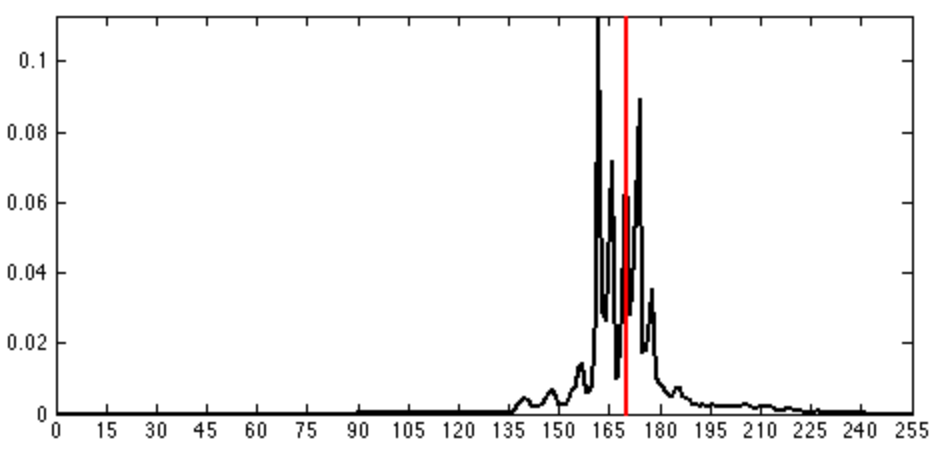
\includegraphics[width=.4\textwidth]{pdf2.png}
\end{figure}
\end{frame}

\begin{frame}
The Otsu's method aims at finding $T$ that maximizes $\sigma_{B}^{2}$, i.~e., best separates the classes:
\begin{figure}[!h]
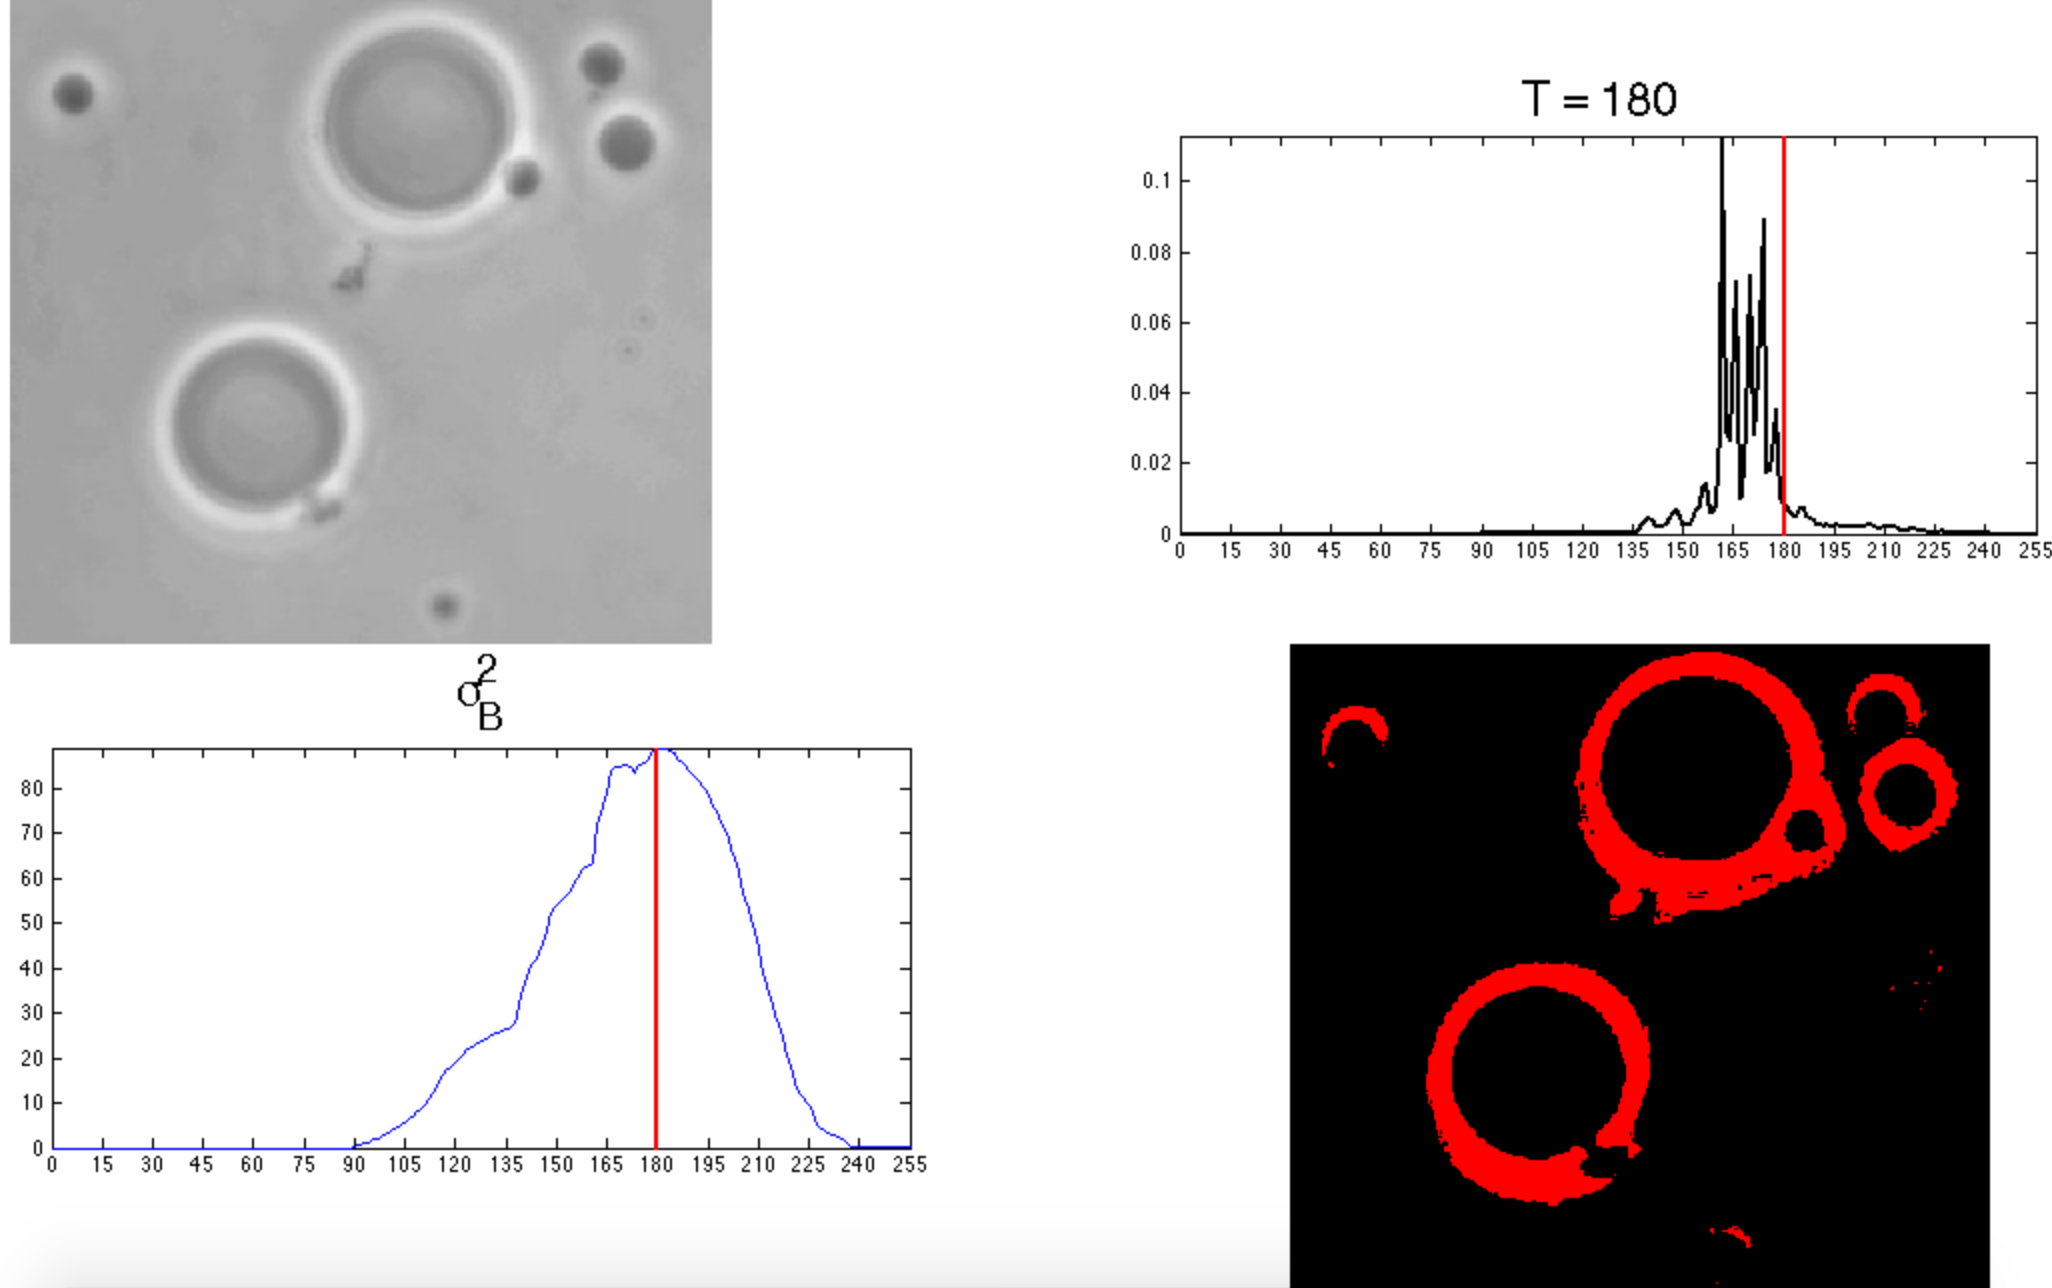
\includegraphics[width=.7\textwidth]{otsu32.png}
\end{figure}
\end{frame}

\subsection{Using image smoothing to improve global thresholding}

\begin{frame}
%\frametitle{Using image smoothing to improve global thresholding}
\begin{figure}[!h]
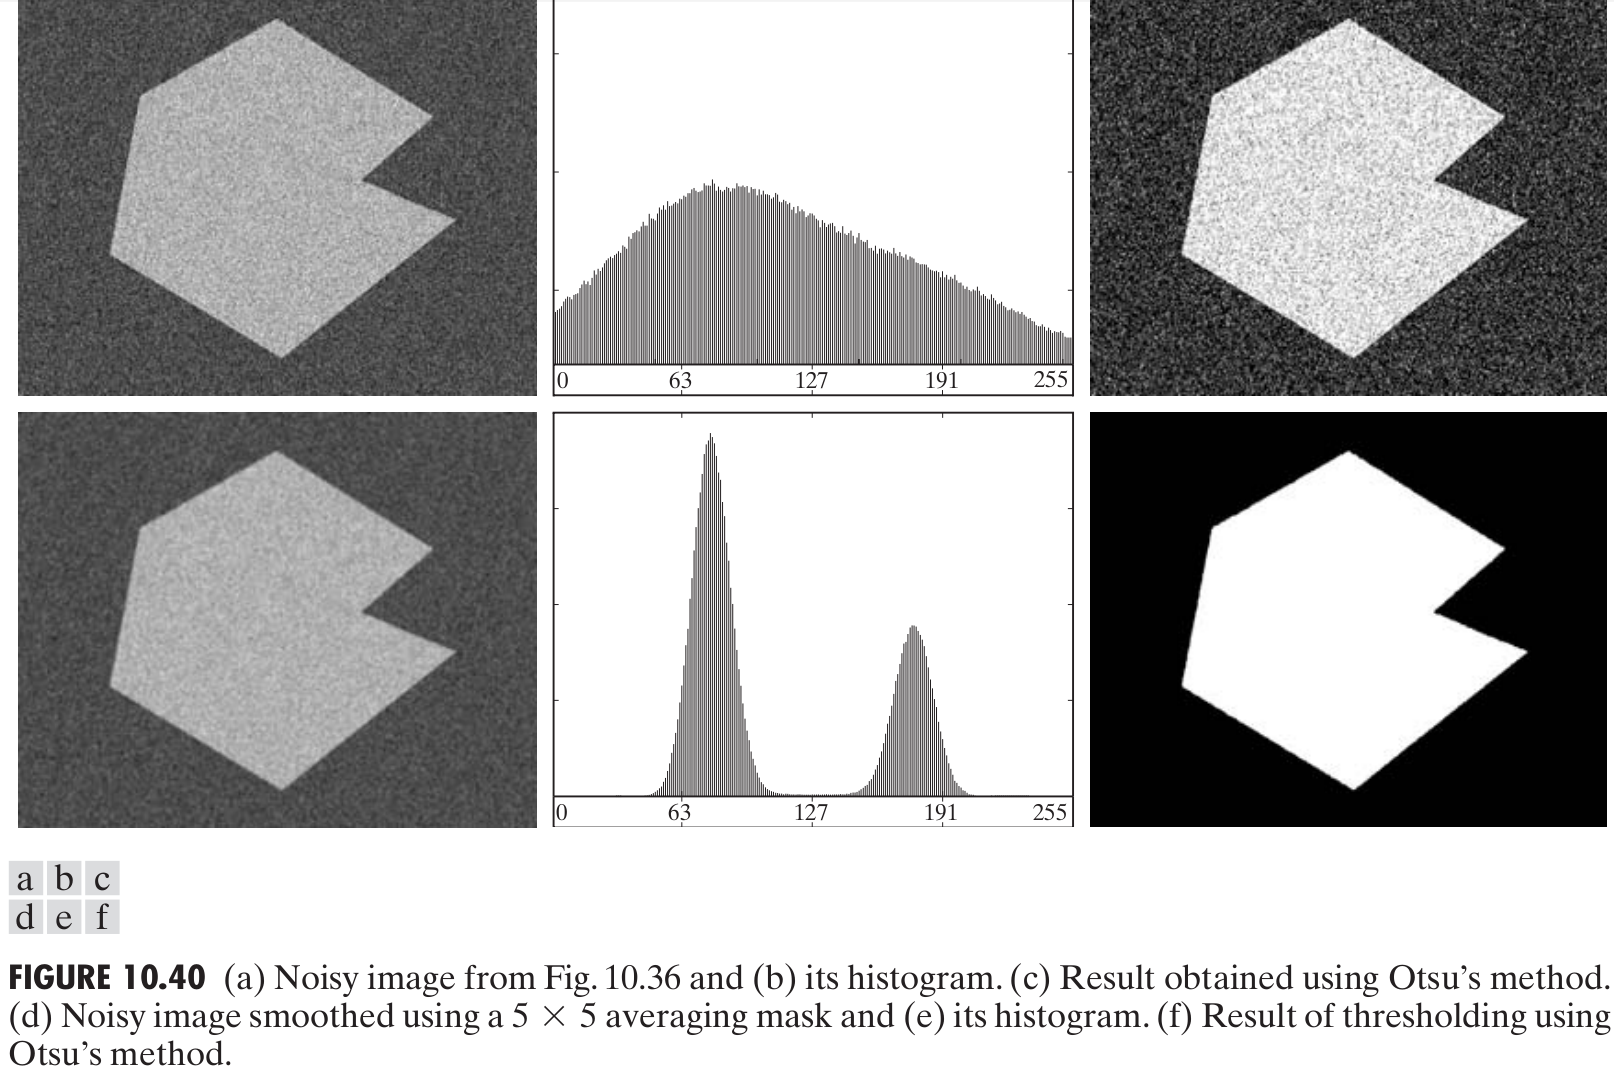
\includegraphics[width=.8\textwidth]{fig-10-40.png}
\end{figure}
\end{frame}

\subsection{Using edges to improve global thresholding}

\begin{frame}
%\frametitle{Using edges to improve global thresholding}
\begin{itemize}
\item A good, separable histogram shape has peaks that are;
\begin{itemize}
\item tall;
\item narrow;
\item symmetric, and;
\item separated by deep valleys.
\end{itemize}
\item One approach to improve histogram shapes is to consider pixels lying on or near edges:
\begin{itemize}
\item less dependency on relative sizes of objects and background.
\item approximately equal probabilities of a pixels lying on object or background.
\item Tendency to deepen the valley between peaks.
\end{itemize}
\end{itemize}
\end{frame}

\section{Region-Based Segmentation}

\subsection{Region Growing}

\begin{frame}[fragile]
\frametitle{Region-Based Segmentation}
\begin{itemize}
\item Region growing is a procedure that groups pixels or sub-regions into larger regions based on predefined criteria for growth.
\item The selection of similarity criteria depends not only on the problem but also on the type of image data available:
\begin{itemize}
\item Analysis of satellite imagery depends heavily on the use of color. Otherwise it would be very difficult.
\item For monochrome images:
\begin{itemize}
\item Use descriptors based on intensity levels (such as moments or texture).
\item spatial properties (such as connectivity).
\end{itemize}
\end{itemize}
\end{itemize}
\end{frame}

\begin{frame}
\begin{itemize}
\item Descriptors can yield misleading results if connectivity is not used in the region-growing process.
\end{itemize}
\begin{block}{Attention}
Criteria such as intensity values, texture, and color, are local in nature and do not take into account the ``history'' of region growth.
\end{block}
\end{frame}

%\begin{frame}[fragile]
%\footnotesize
%\begin{lstlisting}
%n = 3600;
%sampleSize = 200; % choose an even number.
%f = uint8(zeros(sampleSize));
%f2 = f;
%indexes = randi(numel(f), n, 1);
%intensities = uint8(155 + randi(100, n, 1));
%f(indexes) = intensities;
%f2(sampleSize/2 - sqrt(n)/2:sampleSize/2 + sqrt(n)/2 - 1, ...
%    sampleSize/2 - sqrt(n)/2:sampleSize/2 + sqrt(n)/2 - 1) = ...
%    reshape(intensities, sqrt(n), sqrt(n));
%subplot(2,2,1); imshow(f);
%subplot(2,2,2); imshow(f2);
%subplot(2,2,3); imshow(f > 150);
%subplot(2,2,4); imshow(f2 > 150);
%\end{lstlisting}
%\end{frame}
%
%\begin{frame}
%\begin{figure}[!h]
%\centering
%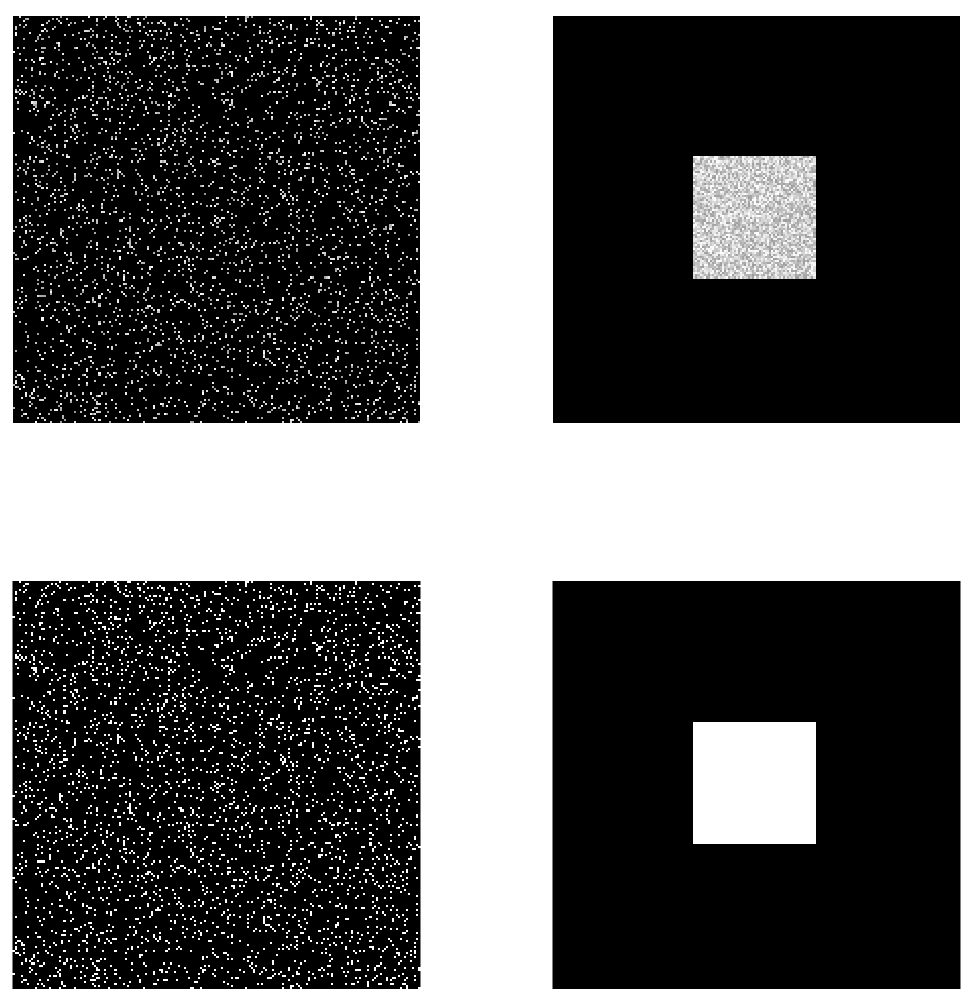
\includegraphics[width=.5\textwidth]{connectivity}
%\end{figure}
%\end{frame}

\begin{frame}[fragile]
\mcode{[g, NR, SI, TI] = regiongrow(f, S, T)}
\begin{itemize}
\item \mcode{f} is the input  image to be segmented.
\item \mcode{S} can be:
\begin{itemize}
\item An array (mask) the same size as \mcode{f}, containing the seed points\footnote{Seeds can be found by inspection or other function.}.
\item A scalar, indicating the intensity value of the pixels to be considered as seeds.
\end{itemize}
\item \mcode{T} can be:
\begin{itemize}
\item An array (same size as \mcode{f}) containing the threshold value for each position in \mcode{f}.
\item A scalar defining a global threshold.
\end{itemize}
\end{itemize}
\begin{block}{Attention}
All values of \mcode{S} and \mcode{T} must be scaled to [0,1].
\end{block}
\end{frame}

\begin{frame}[fragile]
\begin{lstlisting}
%% EXAMPLE 11.13: Using region growing to detect weld porosity.
f = imread('Fig1014(a)(defective_weld).tif');
[g, NR, SI, TI] = regiongrow(tofloat(f), 1, 0.26);
\end{lstlisting}
\begin{figure}[!h]
\centering
\includegraphics[width=.4\textwidth]{weldPorosity.png}
\end{figure}
\end{frame}

\subsection{Region Splitting and Merging}

\begin{frame}%{Region Splitting and Merging}
\begin{enumerate}
\item Split into four disjoint quadrants any region $R_{i}$ for which $Q(R_{i}) = $ FALSE.
\item When no further splitting is possible, merge any adjacent regions $R_{j}$ and $R_{k}$ for which $Q(R_{j} \cup R_{k}) = $ TRUE.
\item Stop when no further merging is possible.
\end{enumerate}
\begin{figure}[!h]
\centering
\includegraphics[width=.7\textwidth]{fig-10-52.png}
\end{figure}
\end{frame}

\begin{frame}[fragile]
\begin{lstlisting}
Z = qtdecomp(f, @split_test, parameters)
\end{lstlisting}
\begin{itemize}
\item \mcode{f} is the input image.
\item \mcode{Z} is a sparse matrix containing the quadtree structure.
\item If $Z(r,c)$ is nonzero, then;
\begin{itemize}
\item $(r,c)$ is the upper-left corner of a block in the decomposition, and;
\item $Z(r,c)$ is the size of the block.
\end{itemize}
\item Function \mcode{split_test} defines the predicate, which determines if a region is to be split or not.
\item \mcode{parameters} are any additional parameters required by the predicate.
\end{itemize}
\end{frame}

\begin{frame}[fragile]
To get the actual quadregion pixel values:
\begin{lstlisting}
[vals, r, c] = qtgetblk(f, Z, m)
\end{lstlisting}
\end{frame}

\begin{frame}
\begin{itemize}
\item X-ray band image of the Cygnus Loop:
\item The objective is to segment out of the image the ``ring'' of less dense matter surrounding the dense center.
\end{itemize}
\begin{figure}[!h]
\centering
\includegraphics[width=.5\textwidth]{cygnusLoop.png}
\end{figure}
\end{frame}

\begin{frame}
\begin{enumerate}
\item The data has a random nature to it.
\item The standard deviation $\sigma$ of the wanted region is greater than the SD of the background ($\sigma=0$) and lower than the brighter region.
\item So the predicate is determined by
\[
Q = 
\left \{
\begin{array}{ll}
\text{TRUE} & \text{if } \sigma > a \text{ AND } 0 < m < b \\
\text{FALSE} & \text{otherwise}
\end{array}
\right ..
\]
\end{enumerate}
\end{frame}

\begin{frame}[fragile]
\begin{lstlisting}
% X-ray band image of the Cygnus Loop.
f = imread('Fig0938(a)(cygnusloop_Xray_original).tif');
mindim = 32; % 32, 16, 8, 4, 2
g = splitmerge(f, mindim, @predicate);
\end{lstlisting}
Where the predicate is defined in a different function
\begin{lstlisting}
function flag = predicate(region)
sd = std2(region);
m = mean2(region);
flag = (sd > 10) & (m > 0) & (m < 125);
\end{lstlisting}
\end{frame}

\begin{frame}
\begin{figure}[!h]
\centering
\includegraphics[width=.5\textwidth]{fig-11-23}
\end{figure}
\end{frame}

\section{Watershed Segmentation}

\begin{frame}
\frametitle{Watershed Segmentation Using The Watershed Transform}
We have discussed segmentation based on three principal concepts:
\begin{itemize}
\item Edge detection (speed).
\item Thresholding (post-processing needed, such as edge linking).
\item Region growing.
\end{itemize}
Let's discuss morphological watersheds. They embody concepts of the previous three approaches.
\end{frame}


\begin{frame}
Visualize the image in three dimensions (topographic interpretation):
\begin{enumerate}
\item Points belonging to a regional minimum.
\item Points at which a drop of water, if placed at the location of any of those points, would fall with certainty to a single minimum.
\item Points at which water would be equally likely to more than one than such minimum.
\end{enumerate}
\begin{figure}[!h]
\centering
\includegraphics[width=\textwidth]{watershed.png}
\end{figure}
\end{frame}


\begin{frame}[fragile]
\begin{lstlisting}
g = bwdist(f)
\end{lstlisting}
\begin{figure}[!h]
\centering
\includegraphics[width=\textwidth]{bwdist.png}
\end{figure}
\end{frame}

\begin{frame}[fragile]
\begin{lstlisting}
g = imread('Fig1020(a)(binary-dowel-image).tif');
gc = ~g;
D = bwdist(gc);
L = watershed(-D);
w = L == 0;
g2 = g & ~w;
\end{lstlisting}
\end{frame}

\begin{frame}
\begin{figure}[!h]
\centering
\includegraphics[width=\textwidth]{watershed1.png}
\end{figure}
\end{frame}

\subsection{Watershed Segmentation Using Gradients}

\begin{frame}[fragile]
\begin{lstlisting}
f = imread('Fig1021(a)(small-blobs).tif');
h = fspecial('sobel');
fd = tofloat(f);
g = sqrt(imfilter(fd, h, 'replicate') .^ 2 + ...
    imfilter(fd, h', 'replicate') .^ 2);

L = watershed(g);
wr = L == 0;

g2 = imclose(imopen(g, ones(3,3)), ones(3,3));
L2 = watershed(g2);
wr2 = L2 == 0;
f2 = f;
f2(wr2) = 255;
\end{lstlisting}
\end{frame}

\begin{frame}
\begin{figure}[!h]
\centering
\includegraphics[width=.6\textwidth]{watershed_example.png}
\end{figure}
\end{frame}

\begin{frame}
\begin{figure}[!h]
\centering
\includegraphics[width=.6\textwidth]{watershed2.png}
\end{figure}
\end{frame}

%\subsection{Marker-Controlled Watershed Segmentation}
%
%\begin{frame}[fragile]
%\begin{lstlisting}
%f0 = imread('Fig1022(a)(gel-image).tif');
%h = fspecial('sobel');
%fd = tofloat(f0);
%g = sqrt(imfilter(fd, h, 'replicate') .^ 2 + ...
%    imfilter(fd, h', 'replicate') .^ 2);
%L = watershed(g);
%wr = L == 0;
%rm = imregionalmin(g);
%\end{lstlisting}
%\end{frame}

%\begin{frame}
%%\frametitle{Using edges to improve global thresholding}
%Compute an edge image from f(x ,y) using any of the methods discussed in Section 11.1. The edge image can be the gradient or the absolute value of the Laplacian.
%2. Specify a threshold value, T.
%3. Threshold the image from step 1 using the threshold from step 2 to pro-
%duce a binary image, gT(X, y).This image is used as a marker image in step 4 to select pixels from f( x , y) corresponding to "strong" edge pixels.
%4. Compute a histogram using only the pixels in f(x,y) that correspond to the locations of the I-valued pixels in gT(X,y).
%5. Use the histogram from step 4 to segment f(x,y) globally using, for example, Otsu's method.
%\end{frame}

%--------------------------------
%-- REFERENCES
%\begin{frame}
%References:
%\begin{itemize}
%\item \href{http://homepages.inf.ed.ac.uk/rbf/HIPR2/open.htm}{http://homepages.inf.ed.ac.uk/rbf/HIPR2/open.htm}
%\end{itemize}
%\end{frame}

\begin{frame}
\frametitle[alignment=center]{}
\flushbottom
\centering
Thank you!\\
\href{mailto:tiago@ic.ufal.br}{tvieira@ic.ufal.br}\\
%\href{mailto:warley.barbosa@edge.ufal.br}{warley.barbosa@edge.ufal.br}\\
%\href{mailto:icaro.bastos@edge.ufal.br}{icaro.bastos@edge.ufal.br}\\
\end{frame}


\end{document}